\documentclass[12pt]{article}

\usepackage{hcmus-report-template}

% Disable indentation on new paragraphs
\setlength{\parindent}{0pt}

% Line spacing 1.5
\renewcommand{\baselinestretch}{1.5}

% Optional: graphic path
% \graphicspath{PATH_TO_GRAPHIC_FOLDER}

% To use Times font family, uncomment this row
% \usepackage{mathptmx}

% To use roman section / subsection, uncomment these rows
% \renewcommand{\thesection}{\Roman{section}}
% \renewcommand{\thesubsection}{\thesection.\Roman{subsection}}

% Define course name, report name and report title.
\newcommand{\coursename}{Cấu trúc dữ liệu và giải thuật}
\newcommand{\reportname}{Các thuật toán sắp xếp}
\newcommand{\reporttitle}{Báo cáo đồ án môn học}

\newcommand{\studentname}{
    Đàm Tiến Đạt (23120118) \\ 
    Huỳnh Cung (23120115) \\
    Võ Hoàng Danh (23120117) \\
    Nguyễn Ngọc Minh Tuấn (23120102) \\
    Nguyễn Phạm Trí Viễn (23120107) \\
}
\newcommand{\teachername}{Trần Hoàng Quân}

% Header
\lhead{\reporttitle}
\rhead{
Trường Đại học Khoa học Tự nhiên - ĐHQG HCM\\
\coursename
}

% Footer
\newcommand{\leftfooter}{\LaTeX\ by \href{https://github.com/magnusdtd}{\textcolor{blue}{Đàm Tiến Đạt}}}
\lfoot{\leftfooter}

% ============ DOCUMENT ============
\begin{document}

\pagenumbering{roman}
\begin{titlepage}
\centering

\textsc{\LARGE đại học quốc gia tphcm}\\[0.5cm]
\textsc{\Large trường đại học khoa học tự nhiên}\\[0.5cm]
\textsc{\large khoa công nghệ thông tin}\\[0.5cm]
\textsc{bộ môn công nghệ tri thức}\\[0.5cm]

\HRule \\[0.2cm]
{ 
\huge{\bfseries{\reporttitle}}\\[0.2cm]
\large{\bfseries{Đề tài: \reportname}}
}\\[0.1cm]
\HRule \\[0.2cm]

\textbf{\large Môn học: \coursename}\\[0.5cm]

\begin{minipage}[t]{0.5\textwidth}
\begin{flushleft} 
\large
\emph{Sinh viên thực hiện:}\\
\studentname
\end{flushleft}
\end{minipage}
~
\begin{minipage}[t]{0.3\textwidth}
\begin{flushleft} \large
\emph{Giáo viên hướng dẫn:} \\
\teachername
\end{flushleft}
\end{minipage}\\[1cm]

{\large \today}\\[1cm]


\includegraphics[scale=.20]{img/hcmus-logo.png}\\[1cm] 

\vfill
\end{titlepage}
	

\tableofcontents
\pagebreak

\pagenumbering{arabic}
\setcounter{page}{1}

\section{Thông tin chung}

\subsection{Giới thiệu sơ lược các thuật toán}

Thuật toán sắp xếp đóng vai trò quan trọng trong khoa học máy tính và các ứng dụng thực tế. Bài báo cáo này tập trung nghiên cứu và so sánh 11 thuật toán sắp xếp phổ biến, bao gồm: Selection Sort, Insertion Sort, Bubble Sort, Shaker Sort, Shell Sort, Heap Sort, Merge Sort, Quick Sort, Counting Sort, Radix Sort, và Flash Sort. Các thuật toán được phân loại thành ba nhóm: thuật toán cơ bản (Selection Sort, Insertion Sort, Bubble Sort, Shaker Sort), thuật toán cải tiến (Shell Sort, Heap Sort, Merge Sort, Quick Sort), và thuật toán không so sánh (Counting Sort, Radix Sort, Flash Sort). Đặc điểm chính, thời gian chạy thực tế và độ phức tạp thời gian của từng thuật toán được phân tích, từ các thuật toán có độ phức tạp $O(n^2)$ đến các thuật toán tối ưu hơn với $O(n \log n)$ hoặc $O(n)$. Kết quả nghiên cứu cung cấp cái nhìn tổng quan về ưu, nhược điểm của từng thuật toán, làm cơ sở cho việc lựa chọn thuật toán phù hợp với các bài toán sắp xếp trong thực tiễn.

\subsection{Dữ liệu}

Dữ liệu sử dụng trong thí nghiệm là mảng số nguyên với các kích thước khác nhau: 10000, 30000, 50000, 100000, 300000, 500000. Tương ứng từng kích thước có 4 kiểu thứ tự của dữ liệu: Mảng được sắp xếp, mảng gần được sắp xếp hoàn chỉnh, mảng được sắp xếp ngược, mảng có thứ tự ngẫu nhiên. Các hàm phát sinh dãy số được giáo viên hướng dẫn thực hành cung cấp trong file \texttt{DataGenerator.cpp}. Tuy nhiên, file \texttt{DataGenerator.cpp} được thay đổi từ sử dụng hàm \textbf{srand} thành hàm \textbf{uniform_int_distribution} của thư viện random c++11. Kết  Các mảng số nguyên phát sinh được yêu cầu sắp xếp tăng dần bằng các thuật toán đề cập trong thí nghiệm.

\subsection{Cấu hình thực nghiệm}
Số liệu thực nghiệm trong báo cáo có được thông qua việc sử dụng GitHub Actions để chạy thực nghiệm. Cấu hình của máy ảo cho một public repository của \href{https://docs.github.com/en/actions/using-github-hosted-runners/using-github-hosted-runners/about-github-hosted-runners#supported-runners-and-hardware-resources}{GitHub}:
\begin{itemize}
    \item CPU: 4 Processor
    \item RAM: 16GB
    \item Storage: 14GB
    \item OS: Ubuntu 24.04.1 LTS
\end{itemize}
 

 


\section{Các thuật toán sắp xếp}

\subsection{Selection sort}

\subsubsection{Ý tưởng}

Thuật toán Selection Sort có ý tưởng khá đơn giản. Dãy đầu vào được chia thành hai phần: phần đã sắp xếp (thường nằm bên trái) và phần chưa sắp xếp (thường nằm bên phải). Thuật toán thực hiện $n - 1$ bước, tại mỗi bước, thuật toán tìm phần tử nhỏ nhất trong phần \textbf{chưa được sắp xếp} và chuyển nó sang \textbf{đã được sắp xếp}. Sau đó tăng kích thước của phần đã sắp xếp thêm 1 và giảm kích thước của phần chưa sắp xếp đi 1.

\subsubsection{Các bước hoạt động}
Xét mảng A như sau: 
\begin{center}
   A = \{5, 9, 0, 3, 7\} 
\end{center} 
Dưới đây là các bước thực hiện thuật toán:

\begin{table}[H]
\centering
\resizebox{\columnwidth}{!}{%
\begin{tabular}{|c|l|l|}
\hline
Giai đoạn & \multicolumn{1}{c|}{Mảng A} & \multicolumn{1}{c|}{Giải thích}                                                                                              \\ \hline
1 &
  \{| 5, 9, \textcolor{red}{0}, 3, 7\} &
  \begin{tabular}[c]{@{}l@{}}Ban đầu phần đã được sắp xếp không có gì, và phần \\ tử bé nhất của phần chưa sắp là 0, đem phần tử 0 \\ lên trước và tăng độ dài của phần được sắp xếp lên\end{tabular} \\ \hline
2         & \{0 | 5, 9, \textcolor{red}{3}, 7\}        & \begin{tabular}[c]{@{}l@{}}Bây giờ phần tử bé nhất của phần chưa sắp là 3, \\đem 3 lên phần đã được sắp xếp\end{tabular}  \\ \hline
3         & \{0, 3 | \textcolor{red}{5}, 9, 7\}        & \begin{tabular}[c]{@{}l@{}}Bây giờ phần tử bé nhất của phần chưa sắp là 5, \\đem 5 lên phần đã được sắp xếp\end{tabular} \\ \hline
4         & \{0, 3, 5 | 9, \textcolor{red}{7}\}        & \begin{tabular}[c]{@{}l@{}}Bây giờ phần tử bé nhất của phần chưa sắp là 7, \\ đem 7 lên phần đã được sắp xếp\end{tabular} \\ \hline
5         & \{0, 3, 5, 7 | 9\}         & \begin{tabular}[c]{@{}l@{}}Tới đây thì thuật toán dừng, không cần đưa phần \\ tử 9 lên trước vì nó đã ở đúng vị trí  \end{tabular}                                         \\ \hline
\end{tabular}%
}
\caption{Các bước thực hiện Selection Sort}
\end{table}

\textcolor{magenta}{Chú thích}: Ký tự “ | ” để phân cách 2 phần đã sắp xếp và chưa sắp xếp của mảng. Phần
tử có màu đỏ chính là phần tử nhỏ nhất của phần chưa được sắp xếp.

\subsubsection{Mã giả}
 
\begin{algorithm}
\caption{Selection Sort}
\label{alg:selection-sort}
\begin{algorithmic}

\Require $A$ is an array of size $n$
\Function {selection-sort}{\textit{A}, \textit{n}}
\For{$i \gets 0$ to $n-2$}
    \State $minIndex \gets i$ \Comment{Assume the current element is the smallest}
    \For{$j \gets i+1$ to $n-1$}
        \If{$A[j] < A[minIndex]$}
            \State $minIndex \gets j$ \Comment{Update the index of the smallest element}
        \EndIf
    \EndFor
    \State Swap $A[i]$ and $A[minIndex]$ \Comment{Place the smallest element at position $i$}
\EndFor
\EndFunction

\end{algorithmic}
\end{algorithm}

\subsubsection{Độ phức tạp}

\textbf{Độ phức tạp thời gian}

Vòng lặp thứ $i$ thực hiện tìm kiếm phần tử nhỏ nhất của phần chưa được sắp xếp (mảng con $A[i,n]$) bằng cách tìm kiếm tuần tự nên tốn $(n-i)$ phép so sánh\footnote{Phần 1, mục 8.2, trang 90 \cite{hoang1999giaithuat}
}.
$$f(n) = 1 + 2 + ... + (n-1) = \frac{n(n-1)}{2} \in O(n^2).$$ 

Chi phí này luôn như nhau không phụ thuộc vào giá trị ban đầu của các phần tử trong mảng.

Do đó độ phức tạp thời gian là\footnote{Mục 5.2.2, trang 196 \cite{dsa_nghia_2013}}:

\begin{itemize}
    \item Trường hợp tốt nhất: $\Omega(n^2)$ (0 đổi chỗ và $\frac{n^2}{2}$ phép so sánh)
    \item Trường hợp tệ nhất: $O(n^2)$ ($n-1$ đổi chỗ và $\frac{n^2}{2}$ phép so sánh)
    \item Trường hợp trung bình: $\Theta(n^2)$ ($O(n)$ đổi chỗ và $\frac{n^2}{2}$ phép so sánh)
\end{itemize}


\textbf{Độ phức tạp không gian}

Thuật toán Selection Sort chỉ tốn một số lượng hằng số các biến trung gian trong tìm kiếm tuần tự và hoán đổi giá trị các phần tử của mảng, nên độ phức tạp không gian cho cả ba trường hợp lần lượt là $O(1), \Omega(1), \Theta(1)$.

 

\subsubsection{Nhận xét}

Ưu điểm nội bật của Selection Sort là số phép đổi chỗ ít. Điều này có ý nghĩa nếu như việc đổi chỗ là tốn kém\footnote{Mục 5.2.2, trang 196 \cite{dsa_nghia_2013}}. 


\textbf{Tính ổn định} 

Vì Selection Sort hoạt động dựa trên việc hoán đổi các phần tử không nằm cạnh nhau), nên nó không đảm bảo thứ tự tương đối của các phần tử có giá trị bằng nhau, và do đó không phải là một thuật toán ổn định.


\textbf{Cải tiến} 

Một cách cải tiến thuật toán này chính là ở mỗi vòng lặp, thay vì chỉ đưa phần tử nhỏ nhất ra trước, đưa thêm phần tử lớn nhất ra phía sau. Mặc dù cải tiến này không giảm độ phức tạp của thuật toán nhưng có thể thấy rằng việc cải tiến này giúp giảm thời gian chạy đi vì số vòng lặp chỉ còn $\frac{n}{2}$ thay vì $n - 1$ vòng lặp như ban đầu.
\subsection{Insertion sort}

\subsubsection{Ý tưởng}

Thuật toán sắp xếp chèn (Insertion Sort) cũng chia mảng thành hai phần tương tự như Selection Sort: phần đã sắp xếp và phần chưa sắp xếp. Thuật toán thực hiện qua $n - 1$ giai đoạn, trong mỗi giai đoạn, nó lấy một phần tử từ phần \textbf{chưa sắp xếp} và tìm vị trí “phù hợp” trong phần \textbf{đã sắp xếp} để chèn vào, đảm bảo phần đã sắp xếp vẫn giữ được trật tự.

\subsubsection{Các bước hoạt động}
Xét mảng A như sau: 
\begin{center}
   A = \{5, 9, 0, 3, 7\} 
\end{center} 
Dưới đây là các bước thực hiện thuật toán:


\begin{table}[H]
\centering
\resizebox{\columnwidth}{!}{%
\begin{tabular}{|c|l|l|}
\hline
Giai đoạn & \multicolumn{1}{c|}{Mảng A} & \multicolumn{1}{c|}{Giải thích}                                                                                              \\ \hline
1 &
  \{5, * | \textcolor{red}{9}, 0, 3, 7\} &
  \begin{tabular}[c]{@{}l@{}}Với thuật toán sắp xếp chèn, phần đã được sắp xếp sẽ\\ bắt đầu với 1 phần tử, và phần tử tiếp theo sẽ được\\ thêm vào là phần tử 9, nó được chèn vào sau số 5\end{tabular} \\ \hline
2         & \{*, 5, 9 | \textcolor{red}{0}, 3, 7\}        & \begin{tabular}[c]{@{}l@{}}Ở giai đoạn này, ta sẽ đưa phần tử 0 lên trước, và vị\\ trí thích hợp là trước số 5\end{tabular}  \\ \hline
3         & \{0, *, 5, 9 | \textcolor{red}{3}, 7\}        & \begin{tabular}[c]{@{}l@{}}Ở giai đoạn này, ta sẽ đưa phần tử 3 lên trước, và vị\\ trí thích hợp là trước số 5.\end{tabular} \\ \hline
4         & \{0, 3, 5, *, 9 | \textcolor{red}{7}\}        & \begin{tabular}[c]{@{}l@{}}Ở giai đoạn này, ta sẽ đưa phần tử 7 lên trước, và vị\\ trí thích hợp là trước số 9.\end{tabular} \\ \hline
5         & \{0, 3, 5, 7, 9 |\}         & Tới đây thì thuật toán dừng                                                                                                  \\ \hline
\end{tabular}%
}
\caption{Các bước thực hiện Insertion Sort}
\end{table}

\textcolor{magenta}{Chú thích}: Ký tự “ | ” để phân cách 2 phần đã sắp xếp và chưa sắp xếp của mảng. Phần tử có màu đỏ chính là phần tử sẽ được chèn lên phần đã được sắp xếp. Vị trí có ký tự “ * ” chính là vị trí thích hợp cho phần tử này.

\subsubsection{Mã giả}
 
\begin{algorithm}
\caption{Insertion Sort}
\label{alg:insertion-sort}
\begin{algorithmic}

\Require $A$ is an array of size $n$
\Function {insertion-sort}{\textit{A}, \textit{n}}
\For{$i \gets 1$ to $n-1$}
    \State $key \gets A[i]$ \Comment{Store the current element}
    \State $j \gets i - 1$
    \While{$j \geq 0$ and $A[j] > key$}
        \State $A[j+1] \gets A[j]$ \Comment{Shift element to the right}
        \State $j \gets j - 1$
    \EndWhile
    \State $A[j+1] \gets key$ \Comment{Insert the element in the correct position}
\EndFor
\EndFunction

\end{algorithmic}
\end{algorithm}

\subsubsection{Độ phức tạp}
\paragraph{Độ phức tạp thời gian}
Trường hợp tốt nhất ứng với mảng đầu vào đã sắp xếp rồi, mỗi lượt chỉ cần 1 phép so sánh, và như vậy tổng số phép so sánh được thực hiện là $n - 1$. Phân tích trong trường hợp tốt nhất, độ phức tạp tính toán của Insertion Sort là $\Omega(n)$.

Trường hợp tệ nhất ứng với mảng đầu vào đã có thứ tự ngược với thứ tự cần sắp thì ở vị trí thứ $i$, cần có $i - 1$ phép so sánh và tổng số phép so sánh là: 

$$(n-1) + (n-2) + ... + 1 = \frac{n* (n-1)}{2}$$ 

Vậy phân tích trong trường hợp tốt nhất, độ phức tạp tính toán của Insertion Sort là $O(n^2)$.

Trường hợp các giá trị xuất hiện một cách ngẫu nhiên, có thể coi xác suất xuất hiện mỗi giá trị là như nhau, thì có thể coi ở lượt thứ $i$, thuật toán cần trung bình $1 / 2$ phép so sánh và tổng số phép so sánh là: $$\frac{1}{2} + \frac{2}{2} + ... + \frac{n}{2} = \frac{(n + 1) * n}{4}$$
Vậy phân tích trong trường hợp trung bình, độ phức tạp tính toán của Insertion Sort là $\Theta(n^2)$\footnote{Phần 1, mục 8.4, trang 91 \cite{hoang1999giaithuat}}.

\paragraph{Độ phức tạp không gian}
Thuật toán Insertion Sort chỉ tốn một số lượng hằng số các biến trung gian trong tìm kiếm tuần tự và hoán đổi giá trị các phần tử của mảng, nên độ phức tạp không gian cho cả ba trường hợp lần lượt là $O(1), \Omega(1), \Theta(1)$.


\subsubsection{Nhận xét}

Insertion Sort là thuật toán sắp xếp tốt đối với mảng đã gần được sắp xếp, nghĩa là mỗi phần từ đã đứng ở vị trí rất gần vị trí trong thứ tự cần sắp xếp\footnote{Mục 5.2.1, trang 195 \cite{dsa_nghia_2013}}. Ngoài ra, Insertion Sort là một thuật toán hiệu quả đối với mảng có kích thước nhỏ ($n <=20$)\footnote{Trang 315 \cite{dsa-analysis-cpp}}.

\paragraph{Tính ổn định}
Trong mỗi bước, Insertion Sort lấy một phần tử từ phần chưa sắp xếp và so sánh với các phần tử trong phần đã sắp xếp. Khi tìm thấy một vị trí phù hợp để chèn phần tử đó, thuật toán không thực hiện hoán đổi nếu gặp phần tử có giá trị bằng nhau, mà chỉ chèn phần tử mới sau các phần tử có cùng giá trị trong phần đã sắp xếp. Vì vậy, thứ tự tương đối giữa các phần tử bằng nhau được bảo toàn.
Do đó, Insertion Sort là một thuật toán ổn định nhờ cách chèn giữ nguyên thứ tự của các phần tử bằng nhau. 

\paragraph{Cải tiến}
 Có thể cải tiến thuật toán sắp xếp chèn nhờ nhận xét: Khi mảng giá trị $A[1...i-1]$ đã được sắp xếp thì việc tìm vị trí chèn có thể làm bằng thuật toán tìm kiếm nhị phân và kỹ thuật chèn có thể làm bằng các lệnh dịch chuyển vùng nhớ cho nhanh. Tuy nhiên điều đó cũng không làm giảm đi độ phức tạp của thuật toán bởi trong trường hợp xấu nhất, phải mất $n - 1$ lần chèn và lần chèn thứ $i$ phải dịch lùi $i$ giá trị để tạo ra khoảng trống trước khi đẩy giá trị chèn vào chỗ trống đó\footnote{Phần 1, mục 8.4, trang 91 \cite{hoang1999giaithuat}}.


\subsection{Bubble sort}

\subsubsection{Ý tưởng}

Thuật toán sắp nổi bọt (Bubble Sort) sẽ duyệt qua mảng $n - 1$ lần, với mỗi lần duyệt, nếu thấy 2 phần tử kề nhau mà phần tử trước lớn hơn phần tử sau thì thuật toán sẽ hoán vị 2 phần tử đó cho nhau. Sau mỗi lần duyệt thì phần tử lớn nhất hiện tại sẽ được đưa về cuối mảng, và không duyệt phần tử này vào lần sau.

\subsubsection{Các bước hoạt động}
Xét mảng A như sau: 
\begin{center}
   A = \{5, 9, 0, 3, 7\} 
\end{center} 
Dưới đây là các bước thực hiện thuật toán:

\begin{table}[H]
\centering
\resizebox{\columnwidth}{!}{%
\begin{tabular}{|c|l|l|}
\hline
Vòng lặp & \multicolumn{1}{c|}{Mảng A} & \multicolumn{1}{c|}{Giải thích} \\ \hline
1 & \{ \textcolor{red}{5, 9}, 0, 3, 7 | \} & 5 và 9 đang đứng đúng vị trí, tiếp tục. \\ \hline
1 & \{ 5, \textcolor{red}{9, 0}, 3, 7 | \} & 9 và 0 đang đứng sai vị trí, hoán vị 2 phần tử này. \\ \hline
1 & \{ 5, 0, \textcolor{red}{9, 3}, 7 | \} & 9 và 3 đang đứng sai vị trí, hoán vị 2 phần tử này. \\ \hline
1 & \{ 5, 0, 3, \textcolor{red}{9, 7} | \} & 9 và 7 đang đứng sai vị trí, hoán vị 2 phần tử này. \\ \hline
1 & \{ 5, 0, 3, 7 | 9 \} & \begin{tabular}[c]{@{}l@{}}Kết thúc lần lặp đầu tiên ở đây, 9 là phần tử lớn nhất \\ đã được đưa về cuối dãy.\end{tabular} \\ \hline
2 & \{ \textcolor{red}{5, 0}, 3, 7 | 9 \} & 5 và 0 đang đứng sai vị trí, hoán vị 2 phần tử này. \\ \hline
2 & \{ 0, \textcolor{red}{5, 3}, 7 | 9\} & 5 và 3 đang đứng sai vị trí, hoán vị 2 phần tử này. \\ \hline
2 & \{ 0, 3, \textcolor{red}{5, 7} | 9\} & 5 và 7 đang đứng đúng vị trí, tiếp tục. \\ \hline
2 & \{ 0, 3, 5, | 7 , 9\} & Kết thúc vòng lặp thứ 2 ở đây \\ \hline
3 & \{ \textcolor{red}{0, 3}, 5, | 7 , 9\} & 0 và 3 đang đứng đúng vị trí, tiếp tục. \\ \hline
3 & \{ 0, \textcolor{red}{3, 5} | 7 , 9\} & 3 và 5 đang đứng đúng vị trí, tiếp tục. \\ \hline
3 & \{ 0, 3 | 5, 7 , 9\} & Kết thúc vòng lặp thứ 3 ở đây \\ \hline
4 & \{ \textcolor{red}{0, 3} | 5, 7 , 9\} & 0 và 3 đang đứng đúng vị trí, tiếp tục. \\ \hline
4 & \{ | 0, 3, 5, 7 , 9\} & Thuật toán kết thúc \\ \hline
\end{tabular}%
}
\caption{Các bước thực hiện Bubble Sort}

\end{table}

% \begin{table}[H]
% \centering
% \resizebox{\columnwidth}{!}{%
% \begin{tabular}{|c|l|l|}
% \hline
% Vòng lặp & \multicolumn{1}{c|}{Mảng A} & \multicolumn{1}{c|}{Giải thích} \\ \hline
% 1 & \{ \textcolor{red}{5, 9}, 0, 3, 7 | \} & 5 và 9 đang đứng đúng vị trí, tiếp tục. \\ \hline
% 1 & \{ 5, \textcolor{red}{9, 0}, 3, 7 | \} & 9 và 0 đang đứng sai vị trí, hoán vị 2 phần tử này. \\ \hline
% 1 & \{ 5, 0, \textcolor{red}{9, 3}, 7 | \} & 9 và 3 đang đứng sai vị trí, hoán vị 2 phần tử này. \\ \hline
% 1 & \{ 5, 0, 3, \textcolor{red}{9, 7} | \} & 9 và 7 đang đứng sai vị trí, hoán vị 2 phần tử này. \\ \hline
% 1 & \{ 5, 0, 3, 7 | 9 \} & \begin{tabular}[c]{@{}l@{}}Kết thúc lần lặp đầu tiên ở đây, 9 là phần tử lớn nhất \\ đã được đưa về cuối dãy.\end{tabular} \\ \hline
% 2 & \{ \textcolor{red}{5, 0}, 3, 7 | 9 \} & 5 và 0 đang đứng sai vị trí, hoán vị 2 phần tử này. \\ \hline
% 2 & \{ 0, \textcolor{red}{5, 3}, 7 | 9\} & 5 và 3 đang đứng sai vị trí, hoán vị 2 phần tử này. \\ \hline
% 2 & \{ 0, 3, \textcolor{red}{5, 7} | 9\} & 5 và 7 đang đứng đúng vị trí, tiếp tục. \\ \hline
% 2 & \{ 0, 3, 5, | 7 , 9\} & Kết thúc vòng lặp thứ 2 ở đây \\ \hline
% 3 & \{ \textcolor{red}{0, 3}, 5, | 7 , 9\} & 0 và 3 đang đứng đúng vị trí, tiếp tục. \\ \hline
% 3 & \{ 0, \textcolor{red}{3, 5} | 7 , 9\} & 3 và 5 đang đứng đúng vị trí, tiếp tục. \\ \hline
% 3 & \{ 0, 3 | 5, 7 , 9\} & Kết thúc vòng lặp thứ 3 ở đây \\ \hline
% 4 & \{ \textcolor{red}{0, 3} | 5, 7 , 9\} & 0 và 3 đang đứng đúng vị trí, tiếp tục. \\ \hline
% 4 & \{ | 0, 3, 5, 7 , 9\} & Thuật toán kết thúc \\ \hline
% \end{tabular}%
% }
% \caption{Các bước thực hiện Bubble Sort}

% \end{table}

\textcolor{magenta}{Chú thích}: Hai phần tử có màu đỏ chính là hai phần tử đang được so sánh. Ký tự “ | ” để phân chia phần được đã sắp xếp và chưa được sắp xếp.

\subsubsection{Mã giả}
 
\begin{algorithm}[H]
\caption{Bubble Sort}
\label{alg:bubble-sort}
\begin{algorithmic}

\Require $A$ is an array of size $n$
\Function {bubble-sort}{\textit{A}, \textit{n}}
\For {$i = 1$ to $n-1$} \Comment{Outer loop for each pass}
    \For {$j = 0$ to $n-i-1$} \Comment{Inner loop for comparing adjacent elements}
        \If{$A[j] > A[j+1]$} \Comment{Check the order of two adjacent elements}
            \State Swap $A[j]$ and $A[j+1]$ \Comment{Swap if elements are in the wrong order}
        \EndIf
    \EndFor
\EndFor
\EndFunction

\end{algorithmic}
\end{algorithm}

\subsubsection{Độ phức tạp}
 
\textbf{Độ phức tạp thời gian}

Đối với thuật toán sắp xếp nổi bọt, có thể coi phép toán tích cực là phép so sánh $A[j] > A[j + 1]$. Và số lần thực hiện phép so sánh này là:
$$(n-1)+(n-2)+...+1 = \frac{n(n-1)}{2}$$
Vậy thuật toán sắp xếp nổi bọt cũng có độ phức tạp là $O(n^2)$. Bất kể tình trạng dữ liệu vào như thế nào\footnote{Phần 1, mục 8.2, trang 90 \cite{hoang1999giaithuat}}. 

\textbf{Độ phức tạp không gian}

Thuật toán Bubble Sort chỉ tốn một số lượng hằng số các biến trung gian trong tìm kiếm tuần tự và hoán đổi giá trị các phần tử của mảng, nên độ phức tạp không gian cho cả ba trường hợp lần lượt là $O(1), \Omega(1), \Theta(1)$.


\subsubsection{Nhận xét}

Trong Bubble Sort, khi so sánh hai phần có giá trị bằng nhau, thuật toán không hoán đổi hai phần tử này. Do đó, thứ tự của các phần tử có giá trị bằng nhau vẫn được bảo toàn trong quá trình sắp xếp. Vậy Bubble Sort là một thuật toán sắp xếp ổn định.

\textbf{Cải tiến}

Một cải tiến cho thuật toán Bubble Sort là dừng sớm nếu mảng đã được sắp xếp hoàn toàn trong một vòng lặp. Điều này giúp giảm số lần so sánh và hoán đổi, từ đó cải thiện hiệu suất trong những trường hợp mảng gần như đã sắp xếp sẵn.
Một cải tiến khác là Shaker Sort ở mục \ref{subsec:shaker-sort}.
\subsection{Shaker sort}
\label{subsec:shaker-sort}

\subsubsection{Ý tưởng}
Shaker Sort (hay còn gọi là Cocktail Sort) là một thuật toán sắp xếp cải tiến từ Bubble Sort. Thuật toán không chỉ duyệt qua danh sách từ đầu đến cuối như Bubble Sort, mà còn thực hiện việc duyệt ngược lại từ cuối đến đầu, giúp thuật toán có thể "chuyển động" cả hai chiều và giảm số lần cần phải duyệt qua. Mỗi lần "lặp qua" danh sách, thuật toán sẽ thay đổi vị trí các phần tử lớn (hoặc nhỏ, tùy vào chiều duyệt) ra ngoài, và sau đó đổi chiều duyệt để di chuyển các phần tử còn lại.

\subsubsection{Các bước hoạt động}
Xét mảng A như sau: 
\begin{center}
   A = \{5, 9, 0, 3, 7\} 
\end{center} 
Dưới đây là các bước thực hiện thuật toán:


\begin{table}[H]
\centering
\resizebox{\columnwidth}{!}{%
\begin{tabular}{|c|l|l|}
\hline
Vòng lặp & \multicolumn{1}{c|}{Mảng A} & \multicolumn{1}{c|}{Giải thích} \\ \hline
1 & \{ | \textcolor{red}{5, 9}, 0, 3, 7 | \} & 5 và 9 đang đứng đúng vị trí, tiếp tục. \\ \hline
1 & \{ | 5, \textcolor{red}{9, 0}, 3, 7 | \} & 9 và 0 đang đứng sai vị trí, hoán vị 2 phần tử này. \\ \hline
1 & \{ | 5, 0, \textcolor{red}{9, 3}, 7 | \} & 9 và 3 đang đứng sai vị trí, hoán vị 2 phần tử này. \\ \hline
1 & \{ | 5, 0, 3, \textcolor{red}{9, 7} | \} & 9 và 7 đang đứng sai vị trí, hoán vị 2 phần tử này. \\ \hline
1 & \{ | 5, 0, 3, 7 | 9 \} & \begin{tabular}[c]{@{}l@{}}Hoàn thành việc duyệt xuôi từ đầu về cuối, lúc này thêm 9 vào \\ phần đã sắp xếp ở sau và bắt đầu duyệt theo thứ tự ngược lại.\end{tabular} \\ \hline
1 & \{ | 5, 0, \textcolor{red}{3, 7} | 9 \} & 3 và 7 đang đứng đúng vị trí, tiếp tục. \\ \hline
1 & \{ | 5, \textcolor{red}{0, 3}, 7 | 9\} & 0 và 3 đang đứng đúng vị trí, tiếp tục. \\ \hline
1 & \{ | \textcolor{red}{5, 0}, 3, 7 | 9\} & 5 và 0 đang đứng sai vị trí, hoán vị 2 phần tử này. \\ \hline
1 & \{ 0 | 5, 3, 7 | 9\} & \begin{tabular}[c]{@{}l@{}}Hoàn thành việc duyệt ngược từ cuối về đầu, lúc này \\ thêm 0 vào phần đã sắp xếp ở trước. Kết thúc lần lặp 1.\end{tabular} \\ \hline
2 & \{ 0 | \textcolor{red}{5, 3}, 7 | 9\} & 5 và 3 đang đứng sai vị trí, hoán vị 2 phần tử này. \\ \hline
2 & \{ 0 | 3, \textcolor{red}{5, 7} | 9\} & 5 và 7 đang đứng đúng vị trí, tiếp tục. \\ \hline
2 & \{ 0 | 3, 5 | 7, 9\} & \begin{tabular}[c]{@{}l@{}}Hoàn thành việc duyệt xuôi từ đầu về cuối, lúc này thêm 7 vào \\ phần đã sắp xếp ở sau và bắt đầu duyệt theo thứ tự ngược lại.\end{tabular} \\ \hline
2 & \{ 0 | \textcolor{red}{3, 5} | 7, 9\} & 3 và 5 đang đứng đúng vị trí, tiếp tục \\ \hline
2 & \{ 0,  3 | 5 | 7, 9\} & \begin{tabular}[c]{@{}l@{}}Ta hoàn thành việc duyệt ngược từ cuối về đầu, lúc này thêm 3 \\ vào phần đã sắp xếp ở trước.
Ta kết thúc lần lặp 2. \end{tabular} \\ \hline
3 & \{ 0,  3 | | 5, 7, 9\} & \begin{tabular}[c]{@{}l@{}}Hoàn thành việc duyệt xuôi từ đầu về cuối, lúc này thêm 5 vào \\ phần đã sắp xếp ở sau. Lúc này ngừng thuật toán vì mảng đã \\ sắp xếp.\end{tabular} \\ \hline
\end{tabular}%
}
\caption{Các bước thực hiện Shaker Sort}
\end{table}

\textcolor{magenta}{Chú thích}: Hai phần tử có màu đỏ chính là hai phần tử đang được so sánh. Ký tự “ | ” để phân cách phần đã sắp xếp và chưa sắp xếp của mảng, sẽ có 2 ký tự “ | ” vì sẽ có 2 phần đã sắp xếp (là phần đầu mảng và cuối mảng).

\subsubsection{Mã giả}
 
\begin{algorithm}[H]
\caption{Shaker Sort}
\label{alg:shaker-sort}
\begin{algorithmic}

\Require $A$ is an array of size $n$
\Function {shaker-sort}{\textit{A}, \textit{n}}
\State $left \gets 0$ \Comment{Set the left boundary of the array}
\State $right \gets n-1$ \Comment{Set the right boundary of the array}
\State $swapped \gets True$ \Comment{Initialize the swapped flag}

\While{$left < right$ and $swapped$} \State \Comment{Continue sorting until the boundaries cross or no swaps occurred}
    \State $swapped \gets False$ \Comment{Reset the swapped flag for the current pass}
    \For{$i = left$ to $right-1$} \Comment{Traverse from left to right}
        \If{$A[i] > A[i+1]$} \Comment{If the current element is greater than the next element}
            \State Swap $A[i]$ and $A[i+1]$ \Comment{Swap if the elements are in the wrong order}
            \State $swapped \gets True$ \Comment{Set the swapped flag}
        \EndIf
    \EndFor
    \State $right \gets right - 1$ \Comment{Decrease the right boundary after the forward pass}

    \If{$swapped$} \Comment{Check if any swaps occurred in the forward pass}
        \State $swapped \gets False$ \Comment{Reset the swapped flag for the backward pass}
        \For{$i = right$ to $left+1$} \Comment{Traverse from right to left}
            \If{$A[i] < A[i-1]$} \Comment{If the current element is less than the previous element}
                \State Swap $A[i]$ and $A[i-1]$ \Comment{Swap if the elements are in the wrong order}
                \State $swapped \gets True$ \Comment{Set the swapped flag}
            \EndIf
        \EndFor
        \State $left \gets left + 1$ \Comment{Increase the left boundary after the backward pass}
    \EndIf

\EndWhile
\EndFunction

\end{algorithmic}
\end{algorithm}


\subsubsection{Độ phức tạp}

\paragraph{Độ phức tạp thời gian}\cite{shaker_sort_cite}

\begin{itemize}
    \item Trong trường hợp xấu nhất: Đối với một mảng có n phần tử, thuật toán Shaker Sort sẽ duyệt qua mảng nhiều lần. Trong mỗi lần duyệt, thuật toán sẽ thực hiện $n$ phép so sánh và hoán đổi, do đó độ phức tạp trong trường hợp xấu nhất là: $O(n^2)$.
    \item Trong trường hợp trung bình: Cũng có độ phức tạp tương tự, khoảng $O(n^2)$, vì thuật toán vẫn phải thực hiện nhiều hoán đổi trong mỗi lần duyệt.
    \item Trong trường hợp tốt nhất: Nếu mảng đã được sắp xếp, thuật toán sẽ chỉ thực hiện một lần duyệt từ trái sang phải và từ phải sang trái, nên độ phức tạp sẽ là $O(n)$.
\end{itemize}

\paragraph{Độ phức tạp không gian}

Shaker Sort chỉ sử dụng một vài biến phụ để lưu trữ chỉ số trái phải và không cần bộ nhớ phụ trợ ngoài mảng ban đầu, vì vậy độ phức tạp không gian cho cả ba trường hợp lần lượt là $O(1), \Omega(1), \Theta(1)$.

\subsubsection{Nhận xét}

\paragraph{Tính ổn định} Tương tự như Bubble Sort, khi so sánh và hoán đổi các phần tử, nếu hai phần tử có giá trị bằng nhau thì không bị hoán đổi, do đó, thứ tự ban đầu của hai phần tử này vẫn được bảo tồn trong quá trình sắp xếp. Vậy Shaker Sort là một thuật toán sắp xếp ổn định.

% \paragraph{Cải tiến}

% Cải tiến bằng cách thêm 1 cờ hiệu (flag) để có thể dừng sớm khi không có hoán đổi nào xảy ra. Lúc này độ phức tạp thời gian trong trường hợp tốt nhất là $\Omega(n)$.
\subsection{Shell sort}

\subsubsection{Ý tưởng}
Thuật toán Shell Sort là một thuật toán sắp xếp được phát triển bởi Donald Shell vào năm 1959. Đây là một cải tiến của thuật toán sắp xếp chèn (Insertion Sort), nhằm giảm thiểu số lần di chuyển phần tử khi danh sách chưa được sắp xếp gần như hoàn chỉnh.
Nguyên lý hoạt động của shell sort là chia danh sách thành các nhóm con, dựa trên dãy khoảng cách $h_1, h_2, \dots, h_t$. Các phần tử trong mỗi nhóm được sắp xếp bằng cách sử dụng phương pháp Insertion Sort. Dãy khoảng cách thường được sử dụng là dãy do chính tác giả đề xuất: $h_1 = n / 2$, $h_i = h_{i + 1} / 2$.

\subsubsection{Các bước hoạt động}
Xét mảng A như sau: 
\begin{center}
   A = \{5, 9, 0, 3, 7\} 
\end{center} 
Dưới đây là các bước thực hiện thuật toán:

\begin{table}[H]
\centering
\resizebox{\columnwidth}{!}{%
\begin{tabular}{|c|l|l|}
\hline
Gap & \multicolumn{1}{c|}{Mảng A} & \multicolumn{1}{c|}{Giải thích} \\ \hline
2   & \{ \textcolor{red}{5}, 9, \textcolor{red}{0}, 3, 7  \} & 5 và 0 đang đứng sai vị trí, hoán vị 2 phần tử này. \\ \hline
2   & \{ 0, \textcolor{red}{9}, 5, \textcolor{red}{3}, 7  \} & 9 và 3 đang đứng sai vị trí, hoán vị 2 phần tử này. \\ \hline
2   & \{ 0, 3, \textcolor{red}{5}, 9, \textcolor{red}{7}   \} & 5 và 7 đang đứng đúng vị trí, tiếp tục. \\ \hline
2   & \{ 0, 3, 5, 9, 7  \} & \begin{tabular}[c]{@{}l@{}}Hoàn thành việc duyệt xuôi từ đầu về cuối, giảm \\ gap xuống còn 1.\end{tabular} \\ \hline
1   & \{ \textcolor{red}{0, 3}, 5, 9, 7 \} & 0 và 3 đang đứng đúng vị trí, tiếp tục. \\ \hline
1   & \{ 0, \textcolor{red}{3, 5}, 9, 7  \} & 3 và 5 đang đứng đúng vị trí, tiếp tục. \\ \hline
1   & \{ 0, 3, \textcolor{red}{5, 9}, 7 \} & 5 và 9 đang đứng đúng vị trí, tiếp tục. \\ \hline
1   & \{ 0, 3, 5, \textcolor{red}{9, 7}\} & 9 và 7 đang đứng sai vị trí, hoán vị 2 phần tử này. \\ \hline
1   & \{ 0, 3, 5, 7, 9 \} & \begin{tabular}[c]{@{}l@{}}Kết thúc thuật toán.\end{tabular} \\ \hline
\end{tabular}%
}
\caption{Các bước thực hiện Shell Sort}
\end{table}

\textcolor{magenta}{Chú thích}: Phần tử màu đỏ chính là phần tử đang được xét.


\subsubsection{Mã giả}
 
\begin{algorithm}[H]
\caption{Shell Sort}
\label{alg:shell-sort}
\begin{algorithmic}

\Require $A$ is an array of size $n$
\Function {shell-sort}{\textit{A}, \textit{n}}
\State $gap \gets \lfloor n / 2 \rfloor$ \Comment{Initialize the gap value}
\While{$gap > 0$} \Comment{Continue sorting while the gap is greater than 0}
    \For{$i = gap$ to $n-1$} \Comment{Traverse the array starting from the gap index}
        \State $temp \gets A[i]$ \Comment{Store the current element}
        \State $j \gets i$
        \While{$j \geq gap$ \textbf{and} $A[j-gap] > temp$} \Comment{Shift elements if out of order}
            \State $A[j] \gets A[j-gap]$ \Comment{Move the element at index $j-gap$ to index $j$}
            \State $j \gets j - gap$
        \EndWhile
        \State $A[j] \gets temp$ \Comment{Place the stored element in its correct position}
    \EndFor
    \State $gap \gets \lfloor gap / 2 \rfloor$ \Comment{Reduce the gap for the next iteration}
\EndWhile
\EndFunction

\end{algorithmic}
\end{algorithm}


% ============================================================================
\subsubsection{Độ phức tạp}

\textbf{Độ phức tạp thời gian} 

Shell Sort hoạt động hiệu quả và cài đặt dễ dàng. Tuy nhiên độ phức tạp của thuật toán này khó để đánh giá một cách chặt chẽ.

\textbf{Sau đây là phần chứng minh cho trường hợp tệ nhất}\footnote{Phần 7.4 Shell Sort, trang 298 \cite{dsa-analysis-cpp}}:

Đầu tiên, chọn $n$ là một lũy thừa của 2. Điều này làm cho tất cả các $h_i$ đều chẵn, ngoại trừ $h_i$ cuối cùng, là 1. Bây giờ, chúng ta sẽ đưa vào một mảng với $n/2$ số lớn nhất ở các vị trí chẵn và $n/2$ số nhỏ nhất ở các vị trí lẻ. Vì tất cả các $h_i$ ngoại trừ $h_i$ cuối cùng đều chẵn, khi chúng ta đến lần lặp cuối cùng, $n/2$ số lớn nhất vẫn nằm ở tất cả các vị trí chẵn và $n/2$ số nhỏ nhất vẫn nằm ở tất cả các vị trí lẻ. Do đó, số thứ $i$ nhỏ nhất ($i\leq n/2$) nằm ở vị trí $2i - 1$ trước khi bắt đầu lần lặp cuối cùng. Khôi phục phần tử thứ $i$ về vị trí chính xác của nó đòi hỏi phải di chuyển nó $i-1$ khoảng trống trong mảng. Do đó, để chỉ đơn thuần đặt $n/2$ phần tử nhỏ nhất vào đúng vị trí sẽ yêu cầu ít nhất $\sum_{i=0}^{n/2 - 1}i=O(n^{2})$ công việc.

 Như chúng ta đã quan sát trước đó, một lần lặp với $h_k$ bao gồm $h_k$ sắp xếp chèn của khoảng $n/h_k$ phần tử. Tổng chi phí của một lần lặp là $O(h_k(n/h_k)^2)=O(n^2/h_k).$ Cộng dồn qua tất cả các lần lặp cho giới hạn tổng là $O(\sum_{i=1}^{t}n^2/h_i)=O(n^2\sum_{i=1}^{t}1/h_i).$ Vì các $h_i$ tạo thành một chuỗi hình học với tỉ số chung là 2 và số hạng lớn nhất trong chuỗi là $h_1=1$, $\sum_{i=1}^{t}1/h_i<2$ Do đó chúng ta thu được giới hạn tổng là $O(n^2)$.

Tóm lại, độ phức tạp thời gian của Shell Sort: 
 \begin{itemize}
    \item Trường hợp tốt nhất: $\Omega(n\log{n})$ 
    \item Trường hợp xấu nhất: $O(n^2)$
    \item Trường hợp trung bình: $\Theta(n\log{n})$
\end{itemize}

\textbf{Độ phức tạp không gian}

Độ phức tạp không gian sẽ là O(1)
% ============================================================================


\subsubsection{Nhận xét}
Trong nhiều trường hợp, đặc biệt là với các mảng lớn và không được sắp xếp hoàn toàn, Shell Sort có thể hoạt động nhanh hơn đáng kể so với sắp xếp chèn. Thuật toán có cấu trúc rõ ràng và dễ hiểu, dễ dàng viết mã để thực hiện. 
Độ phức tạp thời gian của Shell Sort phụ thuộc rất nhiều vào cách chọn dãy các giá trị bước nhảy. Mặc dù trong nhiều trường hợp, nó hoạt động rất tốt, nhưng trong một số trường hợp xấu nhất, độ phức tạp thời gian có thể lên đến $O(n^2)$.

% \textbf{Tính ổn định}


\textbf{Cải tiến}


Có nhiều dãy khác được chứng minh là hiệu quả hơn so với dãy do tác giả đề xuất, giúp giảm độ phức tạp của thuật toán như: Hibbard, Sedgewick, Pratt... Ngoài ra, có thể cải tiến thuật toán sắp xếp chèn bằng cách sử dụng thuật toán khác như binary insertion sort để giảm số lần so sánh và hoán đổi.


\subsection{Heap Sort}

\subsubsection{Ý tưởng}
Heap là một cấu trúc dữ liệu dạng cây nhị phân gần đầy đủ, trong đó các phần tử được sắp xếp theo một quy tắc thứ tự nhất định. Hai loại Heap phổ biến là Max-Heap và Min-Heap. Với Max-Heap, giá trị tại mỗi nút cha lớn hơn hoặc bằng giá trị tại các nút con, trong khi với Min-Heap, giá trị tại mỗi nút cha nhỏ hơn hoặc bằng giá trị tại các nút con.
Heap Sort là một thuật toán sắp xếp dựa trên cấu trúc dữ liệu Heap. Max-heap được sử dụng để sắp xếp mảng tăng dần và Min-Heap được sử dụng để sắp xếp mảng giảm dần. Quá trình sắp xếp được thực hiện qua hai giai đoạn chính: 
\begin{itemize}
    \item Giai đoạn 1: Xây dựng Max-Heap/Min-Heap.
    \item Giai đoạn 2: Lặp lại việc đem phần tử ở gốc Max-Heap/Min-Heap ra cuối/đầu mảng và điều chỉnh lại heap.
\end{itemize}

\subsubsection{Các bước hoạt động}
Xét mảng A như sau: 
\begin{center}
   A = \{5, 9, 0, 3, 7\} 
\end{center} 
Dưới đây là các bước thực hiện giai đoạn 1 - xây dựng Max-Heap:

\begin{table}[H]
\centering
\resizebox{\columnwidth}{!}{%
\begin{tabular}{|c|l|l|}
\hline
\multicolumn{1}{|r|}{Ví trí đang xét} & \multicolumn{1}{c|}{Mảng A} & \multicolumn{1}{c|}{Giải thích} \\ \hline
1 & \{ 5, \textcolor{red}{9}, 0, \textcolor{blue}{3}, \textcolor{blue}{7} \} & \begin{tabular}[c]{@{}l@{}}Đầu tiên do 3 và 7 đều nhỏ hơn 9 nên không thay đổi \\ vị trí của các số trong mảng.\end{tabular} \\ \hline
0 & \{ \textcolor{red}{5}, \textcolor{blue}{9}, \textcolor{blue}{0}, 3, 7 \} & Phần tử 9 lớn hơn 5 và 0 nên hoán đổi vị trí của 5 và 9. \\ \hline
1 & \{ 9, \textcolor{red}{5}, 0, \textcolor{blue}{3}, \textcolor{blue}{7} \} & Phần tử 5 nhỏ hơn 7 nên hoán đổi 5 và 7. \\ \hline
 & \{ 9, 7, 0, 3, 5 \} & Hoàn thành xây dựng Max-Heap. \\ \hline
\end{tabular}%
}
\caption{Các bước xây dựng Max-Heap}
\end{table}


\textcolor{magenta}{Chú thích}: Phần tử màu đỏ chính là phần tử đang được xét, phần tử màu xanh chính là con của phần tử đang xét.

Các bước thực hiện giai đoạn 2 cho mảng A:

\begin{table}[H]
\centering
\resizebox{\columnwidth}{!}{%
\begin{tabular}{|c|l|l|}
\hline
\multicolumn{1}{|r|}{Lần lặp} & \multicolumn{1}{c|}{Mảng A} & \multicolumn{1}{c|}{Giải thích} \\ \hline
1 & \{ \textcolor{red}{9}, 7, 0, 3, 5 | \} & \begin{tabular}[c]{@{}l@{}}Đầu tiên ta đem phần tử 9 về cuối mảng vào phần đã sắp xếp, \\ sau đó đem phần tử 5 lên thay thế phần tử 9.\end{tabular} \\ \hline
1 & \{ \textcolor{red}{5}, \textcolor{blue}{7}, \textcolor{blue}{0}, 3 | 9 \} & Hoán vị phần tử 5 và 7 do 5 < 7. \\ \hline
1 & \{ 7, \textcolor{red}{5}, 0, \textcolor{blue}{3} | 9 \} & Phần tử 5 và 3 đứng đúng vị trí nên không hoán đổi. \\ \hline
2 & \{ \textcolor{red}{7}, 5, 0, \textcolor{red}{3} | 9 \} & \begin{tabular}[c]{@{}l@{}}Sau khi hiệu chỉnh xong, hoán vị phần tử 7 và 3. Đưa phần \\ tử 7 vào phần đã sắp xếp.\end{tabular} \\ \hline
2 & \{\textcolor{red}{3}, \textcolor{blue}{5}, \textcolor{blue}{0} | 7, 9\} & Hoán vị phần tử 3 và 5 do 3 < 5. \\ \hline
3 & \{\textcolor{red}{5}, 3, \textcolor{red}{0} | 7, 9\} & Hoán vị phần tử 5 và 0, đưa phần tử 5 vào phần đã sắp xếp. \\ \hline
3 & \{\textcolor{red}{0}, \textcolor{blue}{3} | 5, 7, 9\} & Hoán vị phần tử 0 và 3 do 0 < 3. \\ \hline
4 & \{\textcolor{red}{3}, \textcolor{red}{0} | 5, 7, 9\} & Hoán vị phần tử 3 và 0, đưa phần tử 3 vào phần đã sắp xếp. \\ \hline
4 & \{\textcolor{red}{0} | 3, 5, 7, 9\} & Phần tử 0 đứng đúng vị trí. \\ \hline
5 & \{0, 3, 5, 7, 9\} & \begin{tabular}[c]{@{}l@{}}Đưa phần tử 0 và\\ phần đã sắp xếp, kết thúc thuật toán\end{tabular} \\ \hline
\end{tabular}%
}
\caption{Các bước sắp xếp sau khi xây dựng Max-Heap của Heap Sort}
\end{table}

\textcolor{magenta}{Chú thích}: Ký tự “ | ” để phân tách mảng thành 2 phần, phần Max-Heap và phần đã được sắp xếp. Phần tử màu đỏ chính là phần tử đang được xét, phần tử màu xanh chính là con của phần tử đang xét. 


\subsubsection{Mã giả}
 
\begin{algorithm}[H]
\caption{Heap Sort}
\label{alg:heap-sort}
\begin{algorithmic}

\Require $A$ is an array of size $n$

\Function {max-heapify}{\textit{A}, \textit{i}, \textit{n}}
\State $largest \gets i$
\State $left \gets 2i + 1$, $right \gets 2i + 2$
\If{$left < n$ \textbf{and} $A[left] > A[largest]$}
    \State $largest \gets left$
\EndIf
\If{$right < n$ \textbf{and} $A[right] > A[largest]$}
    \State $largest \gets right$
\EndIf
\If{$largest \neq i$}
    \State Swap $A[i]$ and $A[largest]$
    \Call{max-heapify}{A, largest, n}
\EndIf
\EndFunction \State

\Function {build-max-heap}{\textit{A}, \textit{n}}
\For{$i = \lfloor n/2 \rfloor - 1$ to $0$}
    \Call{max-heapify}{A, i, n}
\EndFor
\EndFunction \State


\Function {heap-sort}{\textit{A}, \textit{n}}
\State \Call{build-max-heap}{A, n} \Comment{Build a max heap from the array}
\For{$i = n-1$ to $1$}
    \State Swap $A[0]$ and $A[i]$ \Comment{Move the largest element to the end}
    \State $n \gets n - 1$ \Comment{Reduce the size of the heap}
    \State \Call{max-heapify}{A, 0, n} \Comment{Restore the max-heap property}
\EndFor
\EndFunction


\end{algorithmic}
\end{algorithm}


\subsubsection{Độ phức tạp}
\textbf{Độ phức tạp thời gian} Phân tích các bước trong thuật toán:

\begin{itemize}
    \item Xây dựng Max-Heap: Để xây dựng Max-Heap từ mảng, gọi hàm heapify từ vị trí giữa mảng trở về đầu (từ $\left\lfloor \frac{n}{2} \right\rfloor$ đến 0). Mỗi lần gọi heapify có độ phức tạp là $O(\log{n})$ và gọi hàm này cho tất cả các phần tử trong mảng, dẫn đến tổng độ phức tạp là $O(n)$.
    \item Sắp xếp: Sau khi xây dựng, thực hiện $n-1$ lần hoán đổi và mỗi lần hoán đổi lại gọi heapify. Heapify có độ phức tạp là $O(\log{n})$. Vậy độ phức tạp của bước sắp xếp sẽ là $O(n\log{n})$.
\end{itemize}

Kết luận về độ phức tạp thời gian:

 \begin{itemize}
    \item Trường hợp tốt nhất: $\Omega(n)$ (khi mảng có cách phần tử bằng nhau, thao tác hiệu chỉnh có độ phức tạp $O(1)$).
    \item Trường hợp xấu nhất: $O(n\log{n})$
    \item Trường hợp trung bình: $\Theta(n\log{n})$
\end{itemize}

\textbf{Độ phức tạp không gian}

Độ phức tạp không gian là $O(1)$ vì Heap Sort không sử dụng thêm bộ nhớ.

\subsubsection{Nhận xét}

\textbf{Cải tiến} 

Một cách để cải tiến Heap Sort là sử dụng phương pháp Two-Swap. Two-Swap sắp xếp hai phần tử cùng một lúc cho mỗi lần xây dựng Heap. Phương pháp này giảm 30-50\% độ phức tạp thời gian của heapify trong việc xây dựng Heap cũng như trong việc sắp xếp các phần tử mảng. \cite{10.1007/978-3-319-11933-5_78}

\subsection{Merge sort}

\subsubsection{Ý tưởng}
Merge Sort là một thuật toán sắp xếp dựa trên phương pháp "chia để trị". Ý tưởng chính của thuật toán này là liên tục chia nhỏ mảng cần sắp xếp thành các mảng con nhỏ hơn cho đến khi mỗi mảng con chỉ còn một phần tử (đã được sắp xếp). Sau đó, các mảng con này được hợp nhất lại với nhau một cách có thứ tự để tạo thành mảng đã sắp xếp.

Quá trình hoạt động của Merge Sort bao gồm hai bước chính:
\begin{itemize}
    \item Chia: Mảng ban đầu được chia đều thành hai nửa. Quá trình chia này được lặp lại cho đến khi mỗi mảng con chỉ còn một phần tử.
    \item Trộn: Các mảng con được hợp nhất lại thành các mảng lớn hơn một cách có thứ tự. Trong quá trình hợp nhất, các phần tử của hai mảng con được so sánh và chèn vào mảng kết quả theo thứ tự tăng dần (hoặc giảm dần).
\end{itemize}
    
\subsubsection{Các bước hoạt động}
Xét mảng A như sau: 
\begin{center}
   A = \{38, 27, 43, 3, 9, 82, 10\} 
\end{center} 

\textbf{Các bước thực hiện:}

\begin{enumerate}
    \item \textbf{Chia đôi mảng:}
    \begin{itemize}
        \item Chia \( A \) thành hai nửa, với \( L \) nhiều phần tử hơn:
        \[
        L = \{38, 27, 43, 3\}, \quad R = \{9, 82, 10\}.
        \]
        \item Tiếp tục chia đệ quy:
        \[
        L \rightarrow \{38, 27\}, \{43, 3\}, \quad R \rightarrow \{9, 82\}, \{10\}.
        \]
        \item Lặp lại đến khi mỗi mảng chỉ còn một phần tử:
        \[
        L = \{38\}, \{27\}, \{43\}, \{3\}, \quad R = \{9\}, \{82\}, \{10\}.
        \]
    \end{itemize}
    
    \item \textbf{Trộn hai mảng đã sắp xếp:}
    \begin{itemize}
        \item So sánh các phần tử và trộn lại:
        \[
        \{38\}, \{27\} \rightarrow \{27, 38\}, \quad \{43\}, \{3\} \rightarrow \{3, 43\}.
        \]
        \item Tiếp tục:
        \[
        \{27, 38\}, \{3, 43\} \rightarrow \{3, 27, 38, 43\}, \quad \{9\}, \{82\} \rightarrow \{9, 82\}.
        \]
        \item Trộn nửa lớn hơn:
        \[
        \{9, 82\}, \{10\} \rightarrow \{9, 10, 82\}.
        \]
        \item Cuối cùng:
        \[
        \{3, 27, 38, 43\}, \{9, 10, 82\} \rightarrow \{3, 9, 10, 27, 38, 43, 82\}.
        \]
    \end{itemize}

    \item \textbf{Mảng kết quả:}
    Mảng đã sắp xếp:
    \[
    A = \{3, 9, 10, 27, 38, 43, 82\}.
    \]

\end{enumerate}


\begin{figure}[H]
    \centering
    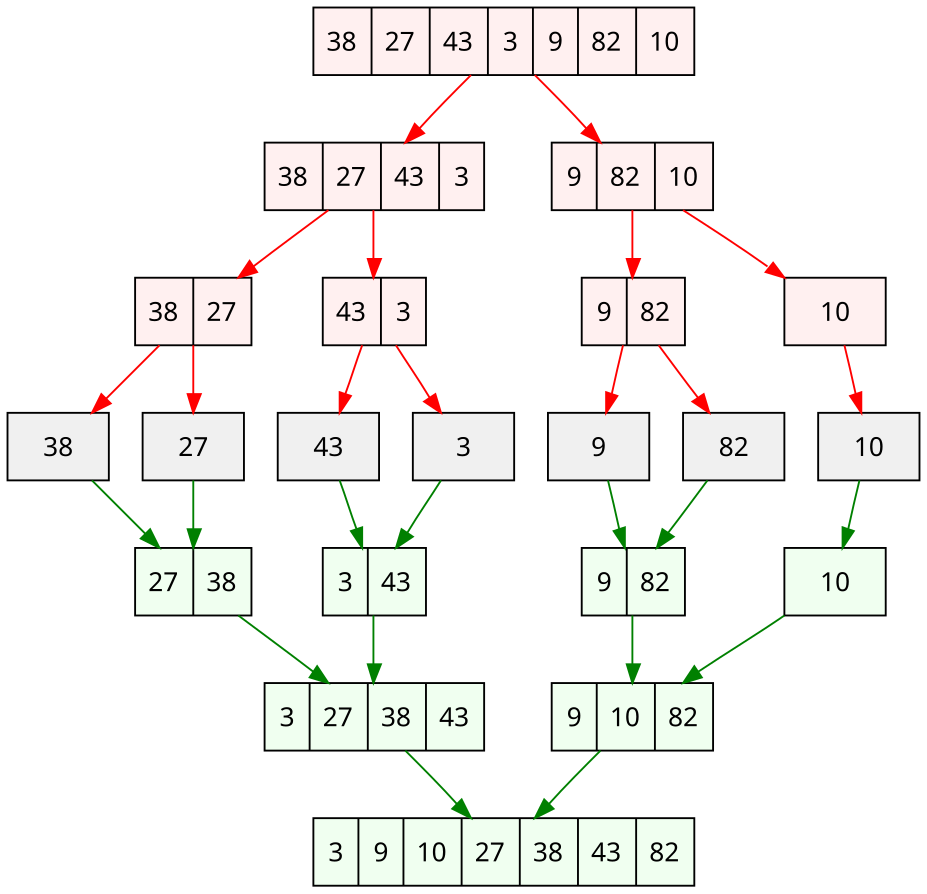
\includegraphics[width=0.8\textwidth]{img/Merge_sort_algorithm_diagram.svg.png}
    \caption{\href{https://en.wikipedia.org/wiki/File:Merge_sort_algorithm_diagram.svg.png}{Merge Sort Algorithm Diagram}}
\end{figure}

\subsubsection{Mã giả}
 
\begin{algorithm}[H]
\caption{Merge Sort}
\label{alg:merge-sort}
\begin{algorithmic}

\Require $A$ is an array of size $n$

\Function {merge}{\textit{A}, \textit{left}, \textit{mid}, \textit{right}}
\State Create temporary arrays $L$ and $R$
\State Copy $A[left \dots mid]$ into $L$, and $A[mid+1 \dots right]$ into $R$
\State Merge $L$ and $R$ back into $A$
\EndFunction \State

\Function {merge-sort}{\textit{A}, \textit{left}, \textit{right}}
\If{$left < right$}
    \State $mid \gets \lfloor (left + right) / 2 \rfloor$ \State
    \Call{merge-sort}{A, left, mid} \Comment{Sort the left half} \State
    \Call{merge-sort}{A, mid+1, right} \Comment{Sort the right half} \State
    \Call{merge}{A, left, mid, right} \Comment{Merge the two halves}
\EndIf
\EndFunction

\end{algorithmic}
\end{algorithm}


\subsubsection{Độ phức tạp}
\paragraph{Độ phức tạp thời gian}\footnote{Chương 7, Merge Sort, trang 307 \cite{dsa-analysis-cpp}}
Gọi $T(n)$ là thời gian thực hiện của thuật toán khi được áp dụng lên một dãy dữ liệu có kích thước $n$.
Giả sử $n$ là một lũy thừa của 2 (n có dạng $2^k$ với $k \in \mathbb{N}^*$), do đó luôn chia mảng ban đầu thành 2 nửa chẵn. Với $n = 1$, thời gian sắp xếp của Merge Sort là hằng số, kí hiệu là 1. Mặt khác, thời gian thực hiện Merge Sort cho $n$ số bằng thời gian thực hiện hai phép sắp xếp hợp nhất đệ quy có kích thước n/2, cộng với thời gian để hợp nhất, là tuyến tính. 

Các phương trình sau đây nói chính xác điều này:

$$\left\{
\begin{array}{l}
        T(1) = 1 \\
        T(n) = T(\frac{n}{2}) + n
\end{array}
\right.$$

Đây là một quan hệ đệ quy chuẩn, có thể được giải theo nhiều cách. Bài báo cáo này sẽ trình bày hai phương pháp. Ý tưởng đầu tiên là chia quan hệ đệ quy cho n. Điều này tạo ra

$$\frac{T(n)}{n} = \frac{T(n / 2)}{n / 2} + 1$$

Phương trình này hợp lệ với bất kỳ n nào là lũy thừa của 2, vì vậy chúng ta cũng có thể viết 

\begin{align*}
    \frac{T(n/2)}{n/2} &= \frac{T(n / 4)}{n / 4} + 1 \\
    \frac{T(n/4)}{n/4} &= \frac{T(n / 8)}{n / 8} + 1 \\
    \dots \\
    \frac{T(2)}{2} &= \frac{T(1)}{1} + 1
\end{align*}

Bây giờ cộng tất cả các phương trình lại. Điều này có nghĩa là cộng tất cả các số hạng ở vế trái và đặt kết quả bằng tổng của tất cả các số hạng ở vế phải. Lưu ý rằng số hạng $T(n/2)/(n/2)$ xuất hiện ở cả hai vế và do đó triệt tiêu. Trên thực tế, hầu như tất cả các số hạng xuất hiện ở cả hai vế và triệt tiêu. Sau khi mọi thứ được cộng lại, kết quả cuối cùng là 

$$\frac{T(n)}{n} = \frac{T(1)}{1} + \log{n}$$

Vì tất cả các số hạng khác triệt tiêu và có $\log{n}$ phương trình, do đó tất cả các số 1 ở cuối các phương trình này cộng lại bằng $\log{n}$. Nhân qua n sẽ cho kết quả cuối cùng. 

$$T(n) = n +  n\log{n}$$

Một phương pháp thay thế là thay thế mối quan hệ đệ quy liên tục ở vế phải.

Ta có 
$$T(n) = 2T(n/2) + n$$

Thay $n/2$ vào phương trình chính:

\begin{align*}
    2T(n/2) &= 2(2T(n/4) + n / 2) = 4T(n/4) + n \\
    \Rightarrow T(n) &= 4T(n / 4) + 2n
\end{align*}

Một lần nữa, bằng cách thay thế $n/4$ vào phương trình chính, ta thấy rằng 

\begin{align*}
    4T(n/4) &= 4(2T(n/8) + n / 4) = 8T(n/8) + n \\
    \Rightarrow T(n) &= 8T(n / 8) + 3n
\end{align*}

Tiếp tục theo cách này, ta thu được

$$T(n) = 2^kT(n/2^k) + kn$$


Sử dụng $k = \log{n}$, ta thu được

$$T(n) = nT(1) + n\log{n} = n\log{n} + n$$

Kết luận về độ phức tạp thời gian:

 \begin{itemize}
    \item Trường hợp tốt nhất: $\Omega(n\log{n})$ 
    \item Trường hợp xấu nhất: $O(n\log{n})$
    \item Trường hợp trung bình: $\Theta(n\log{n})$
\end{itemize}

\paragraph{Độ phức tạp không gian}
Trong bước trộn hai dãy con của Merge Sort có sử dụng mảng phụ để lưu tạm thời các giá trị nên chi phí không gian của giải thuật này là $O(n)$.

\subsubsection{Nhận xét}

Merge Sort là một thuật toán sắp xếp hiệu quả và ổn định, phù hợp với các trường hợp yêu cầu giữ nguyên thứ tự của các phần tử có giá trị bằng nhau. Tuy nhiên, việc sử dụng đệ quy có thể ảnh hưởng đến hiệu suất thực tế. 
\paragraph{Cải tiến}
Một cách cải tiến đó là khử đệ quy (Iterative Merge Sort) giúp  giảm bộ nhớ sử dụng do không gọi đệ quy.
\subsection{Quick sort}

\subsubsection{Ý tưởng}

Quick Sort cũng là một thuật toán sắp xếp dựa trên phương pháp "chia để trị", nhưng cách thức chia và hợp nhất khác so với Merge Sort.
% \begin{itemize}
%     \item Chọn pivot: Đầu tiên, một phần tử trong mảng được chọn làm pivot.
%     \item Phân hoạch: Mảng được chia thành hai phần con:
%     \begin{itemize}
%         \item Các phần tử nhỏ hơn pivot.
%         \item Các phần tử lớn hơn hoặc bằng pivot.
%     \end{itemize}
    
%     \item Đệ quy: Quá trình trên được lặp lại đệ quy cho mỗi phần con cho đến khi mảng con chỉ còn một phần tử hoặc không còn phần tử nào.
% \end{itemize}

Thuật toán quicksort cổ điển để sắp xếp một mảng $A$ bao gồm bốn bước đơn giản sau:

1. Nếu số lượng phần tử trong $A$ là 0 hoặc 1, thì trả về.

2. Chọn bất kỳ phần tử $v$ nào trong $A$. Đây được gọi là phần tử trục (pivot).

3. Phân chia $A - \{v\}$ (các phần tử còn lại trong $A$) thành hai nhóm rời nhau: 
\begin{itemize}
    \item $A_1 = \{x \in A - \{v\} \mid x \leq v\}$
    \item $A_2 = \{x \in A - \{v\} \mid x \geq v\}$.
\end{itemize}

4. Trả về \{ \{$quicksort(A_1)$\}, $v$, \{$quicksort(A_2)$\} \}.

    
    
\subsubsection{Các bước hoạt động}
Xét mảng A như sau: 
\begin{center}
   A = \{5, 3, 8, 4, 6, 3, 2\} 
\end{center} 

Bước 1: Chọn phần tử chốt (pivot) là phần tử chính giữa của mảng là:
\[
\text{Pivot} = 4
\]

Bước 2: Di chuyển các phần tử nhỏ hơn hoặc bằng pivot về bên trái và phần tử lớn hơn về bên phải:
\[
\{3, 3, 2, 4, 5, 8, 6\}
\]

Bước 3: Gọi đệ quy, thực hiện đệ quy Quick Sort trên hai mảng con:
\begin{itemize}
    \item Mảng con bên trái: \(\{3, 3, 2\}\)
    \item Mảng con bên phải: \(\{5, 8, 6\}\)
\end{itemize}

Sắp xếp mảng con bên trái \(\{3, 3, 2\}\):
\begin{itemize}
    \item Chọn pivot: \(3\) (phần tử giữa của mảng con).
    \item Phân hoạch: \(\{2, 3, 3\}\).
    \item Kết quả: \(\{2, 3, 3\}\) (không cần đệ quy thêm).
\end{itemize}

Sắp xếp mảng con bên phải \(\{5, 8, 6\}\):
\begin{itemize}
    \item Chọn pivot: \(8\) (phần tử giữa của mảng con).
    \item Phân hoạch: \(\{5, 6, 8\}\).
    \item Kết quả: \(\{5, 6, 8\}\) (không cần đệ quy thêm).
\end{itemize}

Kết hợp mảng đã sắp xếp
Ghép các mảng con lại:
\[
A = \{2, 3, 3, 4, 5, 6, 8\}
\]

\begin{figure}[H]
    \centering
    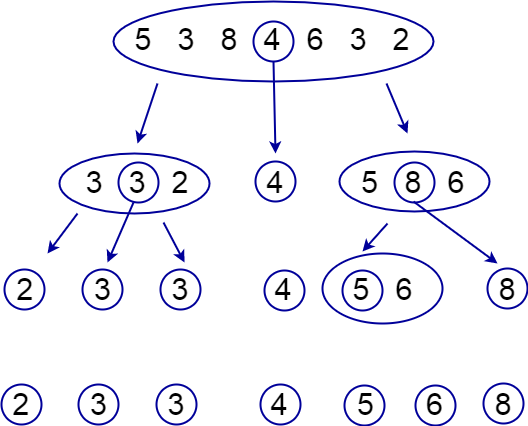
\includegraphics[width=0.8\textwidth]{img/quick_sort.png}
    \caption{\href{https://qnaplus.com/wp-content/uploads/2017/05/quick_sort.png}{Quick Sort Algorithm Diagram}}
\end{figure}

\subsubsection{Mã giả}
 
\begin{algorithm}[H]
\caption{Quick Sort}
\label{alg:quick-sort}
\begin{algorithmic}

\Require $A$ is an array of size $n$

\Function {partition}{\textit{A}, \textit{low}, \textit{high}}
\State $pivot \gets A[high]$
\State $i \gets low - 1$
\For{$j = low$ to $high-1$}
    \If{$A[j] < pivot$}
        \State $i \gets i + 1$
        \State Swap $A[i]$ and $A[j]$
    \EndIf
\EndFor
\State Swap $A[i+1]$ and $A[high]$
\State \Return $i+1$
\EndFunction

\Function {quick-sort}{\textit{A}, \textit{low}, \textit{high}}
\If{$low < high$}
    \State $pivot \gets$ \Call{partition}{A, low, high} \State
    \Call{quick-sort}{A, low, pivot-1} \Comment{Sort the left subarray}
    \State \Call{quick-sort}{A, pivot+1, high} \Comment{Sort the right subarray}
\EndIf
\EndFunction

\end{algorithmic}
\end{algorithm}


\subsubsection{Độ phức tạp}
\paragraph{Độ phức tạp thời gian}
\footnote{Mục 7.7.5 \cite{dsa-analysis-cpp}}Giả sử một pivot ngẫu nhiên và $T(0) = T(1) = 1$. Thời gian chạy của quicksort bằng thời gian chạy của hai lệnh gọi đệ quy cộng với thời gian tuyến tính dành cho phân vùng (lựa chọn pivot chỉ mất thời gian không đổi). Điều này đưa ra mối quan hệ quicksort cơ bản 

\begin{equation}
T(n) = T(i) + T(n - i - 1) + cn \tag{2.8.1} 
\end{equation}

trong đó i là số phần tử của $A_1$. Xét ba trường hợp sau:

\subparagraph{1. Trường hợp xấu nhất}

Pivot là phần tử nhỏ nhất, mọi lúc. Khi đó i = 0, và nếu bỏ qua $ T(0) = 1$, là không đáng kể, thì hệ thức đệ quy là 
$$T(n) = T(n - 1) + cn,  n > 1$$ 								 
Sử dụng phương trình trên nhiều lần. Ta có:
\begin{align*}
T(n - 1) &= T(n - 2) + c(n - 1) \\
T(n - 2) &= T(n - 3) + c(n - 2) \\
\dots \\
T(2) &= T(1) + 2c   
\end{align*}
	 
Cộng tất cả các phương trình này lại, ta được 
$$T(n) = T(1) + c \sum_{i = 2}^{n}i = 1 + c \frac{(n - 1)(n + 2)}{2}$$

Để thấy rằng đây là trường hợp tệ nhất có thể, hãy lưu ý rằng tổng chi phí của tất cả các phân vùng trong các lệnh gọi đệ quy ở độ sâu d phải tối đa là $n$. Vì độ sâu đệ quy tối đa là $n$, điều này đưa ra giới hạn trường hợp tệ nhất là $O(n^2)$ cho Quick Sort.

\subparagraph{2. Trường hợp tốt nhất}

Trong trường hợp tốt nhất, pivot nằm ở giữa. Để đơn giản hóa phép toán, giả sử rằng hai mảng con đều có kích thước bằng đúng một nửa kích thước của mảng ban đầu.

$$T(n) = 2T(n / 2) + cn$$

Chia cả hai vế của phương trình trên cho n. 

$$\frac{T(n)}{n} = \frac{T(n / 2)}{n / 2} + c$$

Tương tự, ta được:
\begin{align*}
    \frac{T(n/2)}{n/2} &= \frac{T(n / 4)}{n / 4} + c \\
    \frac{T(n/4)}{n/4} &= \frac{T(n / 8)}{n / 8} + c \\
    \dots \\
    \frac{T(2)}{2} &= \frac{T(1)}{1} + c
\end{align*}

Chúng ta cộng tất cả các phương trình trên lại và lưu ý rằng có $\log{n}$ phương trình:
\begin{align*}
    \frac{T(n)}{n} &= \frac{T(1)}{1} + c \log{n} \\
    \implies T(n) &= n + cn\log{n} 
\end{align*}

Do đó giới hạn trường hợp tốt nhất là $O(n\log{n})$ cho Quick Sort.

\subparagraph{3. Trường hợp trung bình}
Giả sử rằng mỗi kích thước cho $A_1$ có khả năng xảy ra như nhau và do đó có xác suất là $\frac{1}{n}$. Giả sử này chỉ hợp lệ đối với cách chọn pivot và phân hoạch như trên. 

Với giả định này, giá trị trung bình của $T(i)$, và do đó là $T(n - i - 1)$, là $\frac{1}{n} \sum_{j = 0}^{n - 1}T(j)$. Phương trình  (2.8.1) trở thành: 

\begin{align*}
    & T(n) = \frac{2}{n} \left[\sum_{j = 0}^{n - 1}T(j) \right] + cn \\
    \implies  &nT(n) = 2 \left[\sum_{j = 0}^{n - 1}T(j) \right] + cn^2 \tag{2.8.2} \\
    \implies  &(n - 1)T(n - 1) = 2 \left[\sum_{j = 0}^{n - 2}T(j) \right] + c(n - 1)^2 \tag{2.8.3}
\end{align*}

Lấy phương trình (2.8.2) - (2.8.3), ta được:

$$nT(n)-(n-1)T(n-1)=2T(n-1)+2cn-c $$
Sắp xếp lại các số hạng và bỏ $-c$ không đáng kể ở bên phải, thu được: 

\begin{align*}
    nT(n)=(n+1)T(n-1)+2cn \tag{2.8.4}
\end{align*}

Bây giờ ta có một công thức cho $T(n)$ chỉ theo $T(n - 1)$. Chia phương trình (2.8.4) cho $n(n + 1)$: 

\begin{align*}
&\frac{T(n)}{n+1}=\frac{T(n-1)}{n}+\frac{2c}{n+1} \\
\implies &\frac{T(n-1)}{n}=\frac{T(n-2)}{n-1}+\frac{2c}{n} \\
\implies &\frac{T(n-2)}{n-1}=\frac{T(n-3)}{n-2}+\frac{2c}{n-1} \\
&\dots \\
\implies &\frac{T(2)}{3}=\frac{T(1)}{2}+\frac{2c}{3} \\
\end{align*}

Cộng các phương trình lại, cho kết quả:
\begin{align*}
&\frac{T(n)}{n+1}=\frac{T(1)}{2}+2c\sum_{i=3}^{n+1}\frac{1}{i} \tag{7.23} \\
\end{align*}

Tổng xấp xỉ $\ln(n + 1) + \gamma - 3/2$ , trong đó $\gamma \approx 0,577$ được gọi là hằng số Euler, do đó 

\begin{align*}
    &\frac{T(n)}{n+1}=O(\log n) \\
    \implies &T(n)=O(n \log n) 
\end{align*}


Kết luận về độ phức tạp thời gian:

 \begin{itemize}
    \item Trường hợp tốt nhất: $\Omega(n\log{n})$ 
    \item Trường hợp xấu nhất: $O(n^2)$
    \item Trường hợp trung bình: $\Theta(n\log{n})$
\end{itemize}
\paragraph{Độ phức tạp không gian}
Quick Sort sử dụng số lượng hằng số các biến trung gian trong quá trình hoán đổi các phần tử lúc phân hoạch mảng, do đó độ phức tạp không gian là $O(1)$.


\subsubsection{Nhận xét}

Quick Sort và Merge Sort là hai thuật toán sắp xếp nổi tiếng dựa trên phương pháp chia để trị. Quick Sort thường được đánh giá cao về tốc độ thực thi nhờ việc không sử dụng mảng phụ và cấu trúc đơn giản. Tuy nhiên, hiệu suất của Quick Sort phụ thuộc rất lớn vào việc lựa chọn pivot. Nếu không may chọn phải pivot không phù hợp, thuật toán có thể rơi vào trường hợp xấu nhất với độ phức tạp $O(n^2)$. Ngược lại, Merge Sort luôn đảm bảo độ phức tạp $O(n \log{n})$ trong mọi trường hợp, nhưng thường tiêu tốn nhiều không gian bộ nhớ hơn do cần sử dụng mảng phụ. 

Trong thực tế, Quick Sort được sử dụng rộng rãi trong các thư viện sắp xếp của nhiều ngôn ngữ lập trình nhờ tốc độ nhanh và tính linh hoạt. Tuy nhiên, khi yêu cầu độ ổn định cao hoặc cần xử lý các tập dữ liệu lớn, Merge Sort vẫn là một lựa chọn đáng cân nhắc.

\paragraph{Cải tiến}
Để khắc phục hạn chế về việc chọn pivot của Quick Sort, nhiều phương pháp cải tiến đã được đề xuất như chọn pivot ngẫu nhiên, median-in-medians, . Ngoài ra, các biến thể của Quick Sort giúp cải thiện hiệu suất trong các trường hợp cụ thể như Quick Sort ba đường phân hoạch (chia mảng thành 3 phần), Introsort (một thuật toán sắp xếp hybrid, kết hợp ưu điểm của cả Quick Sort và Heap Sort để đạt được hiệu suất cao trong hầu hết các trường hợp).


\subsection{Counting sort}

\subsubsection{Ý tưởng}
Counting Sort là một thuật toán sắp xếp không dựa trên so sánh, có ưu điểm là tốc độ rất nhanh khi dữ liệu đầu vào thỏa mãn các điều kiện nhất định. Tuy nhiên, thuật toán này có một số hạn chế: chỉ phù hợp với các mảng số nguyên, yêu cầu biết trước khoảng giá trị của các phần tử và tiêu tốn thêm không gian bộ nhớ để tạo mảng đếm.

Có 3 giai đoạn trong thuật toán Counting Sort:
\begin{itemize}
    \item Đếm và phân phối: Tạo một mảng đếm để lưu trữ số lần xuất hiện của mỗi giá trị trong mảng ban đầu. Từ đó, xác định vị trí chính xác của mỗi giá trị trong mảng đã sắp xếp.
    \item Tạo mảng phụ: Tạo một mảng phụ có cùng kích thước với mảng ban đầu. Duyệt mảng ban đầu và đặt từng phần tử vào vị trí chính xác tương ứng trong mảng phụ.
    \item Ghi đè: Ghi đè mảng ban đầu bằng mảng phụ đã sắp xếp.
\end{itemize}


\subsubsection{Các bước hoạt động}
Xét mảng A như sau: 
\begin{center}
   A = \{6, 8, 1, 3, 5, 2\} 
\end{center} 

Bước 1: Xác định giá trị nhỏ nhất và lớn nhất
\[
\text{Min} = 1, \quad \text{Max} = 8
\]

Tạo mảng đếm (\( \text{count} \)) với kích thước \( \text{Max} - \text{Min} + 1 = 8 - 1 + 1 = 8 \):
\[
\text{count} = \{0, 0, 0, 0, 0, 0, 0, 0\}
\]

Bước 2: Đếm số lần xuất hiện của từng phần tử. Duyệt qua mảng \( A \), cập nhật mảng \( \text{count} \):
\[
\begin{aligned}
&\text{A[0] = 6} \quad \Rightarrow \text{count}[6 - 1] = 1 \\
&\text{A[1] = 8} \quad \Rightarrow \text{count}[8 - 1] = 1 \\
&\text{A[2] = 1} \quad \Rightarrow \text{count}[1 - 1] = 1 \\
&\text{A[3] = 3} \quad \Rightarrow \text{count}[3 - 1] = 1 \\
&\text{A[4] = 5} \quad \Rightarrow \text{count}[5 - 1] = 1 \\
&\text{A[5] = 2} \quad \Rightarrow \text{count}[2 - 1] = 1 \\
\end{aligned}
\]

Kết quả:
\[
\text{count} = \{1, 1, 1, 0, 1, 1, 0, 1\}
\]

Bước 3: Tính chỉ số tích lũy trong mảng đếm. Cập nhật \( \text{count} \) thành mảng tích lũy:
\[
\begin{aligned}
\text{count}[1] & = \text{count}[0] + \text{count}[1] = 1 + 1 = 2 \\
\text{count}[2] & = \text{count}[1] + \text{count}[2] = 2 + 1 = 3 \\
\text{count}[3] & = \text{count}[2] + \text{count}[3] = 3 + 0 = 3 \\
\text{count}[4] & = \text{count}[3] + \text{count}[4] = 3 + 1 = 4 \\
\text{count}[5] & = \text{count}[4] + \text{count}[5] = 4 + 1 = 5 \\
\text{count}[6] & = \text{count}[5] + \text{count}[6] = 5 + 0 = 5 \\
\text{count}[7] & = \text{count}[6] + \text{count}[7] = 5 + 1 = 6 \\
\end{aligned}
\]

Kết quả:
\[
\text{count} = \{1, 2, 3, 3, 4, 5, 5, 6\}
\]

Bước 4: Sắp xếp mảng ban đầu vào mảng kết quả. Tạo mảng kết quả \( \text{output} \) với kích thước bằng mảng \( A \). Duyệt ngược qua mảng \( A \) và đặt các phần tử vào đúng vị trí dựa trên mảng \( \text{count} \):
\[
\begin{aligned}
&\text{A[5] = 2} \quad \Rightarrow \text{output}[1] = 2, \quad \text{count}[2 - 1] = 1 \\
&\text{A[4] = 5} \quad \Rightarrow \text{output}[4] = 5, \quad \text{count}[5 - 1] = 4 \\
&\text{A[3] = 3} \quad \Rightarrow \text{output}[2] = 3, \quad \text{count}[3 - 1] = 2 \\
&\text{A[2] = 1} \quad \Rightarrow \text{output}[0] = 1, \quad \text{count}[1 - 1] = 0 \\
&\text{A[1] = 8} \quad \Rightarrow \text{output}[5] = 8, \quad \text{count}[8 - 1] = 5 \\
&\text{A[0] = 6} \quad \Rightarrow \text{output}[3] = 6, \quad \text{count}[6 - 1] = 3 \\
\end{aligned}
\]

Kết quả:
\[
\text{output} = \{1, 2, 3, 5, 6, 8\}
\]

Bước 5: Sao chép mảng \( \text{output} \) vào mảng \( A \).


\begin{figure}[H]
    \centering
    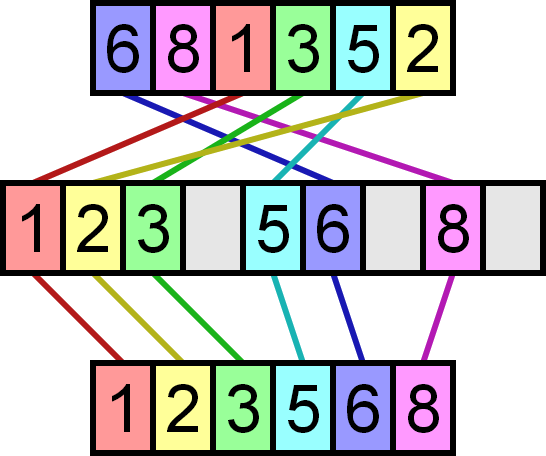
\includegraphics[width=0.8\textwidth]{img/counting-sort.png}
    \caption{\href{https://www.growingwiththeweb.com/images/2014/05/25/counting-sort.svg}{Counting Sort Algorithm Diagram}}
\end{figure}

\subsubsection{Mã giả}
 
\begin{algorithm}[H]
\caption{Counting Sort}
\label{alg:counting-sort}
\begin{algorithmic}

\Require $A$ is an array of size $n$ with integers in the range $0$ to $k$
\Function {counting-sort}{\textit{A}, \textit{k}}
\State Initialize $count[0 \dots k]$ to $0$
\For{$i = 0$ to $n-1$}
    \State $count[A[i]] \gets count[A[i]] + 1$
\EndFor
\For{$i = 1$ to $k$}
    \State $count[i] \gets count[i] + count[i-1]$
\EndFor
\For{$i = n-1$ to $0$}
    \State $B[count[A[i]]-1] \gets A[i]$
    \State $count[A[i]] \gets count[A[i]] - 1$
\EndFor
\State \Return $B$
\EndFunction

\end{algorithmic}
\end{algorithm}


\subsubsection{Độ phức tạp}
\paragraph{Độ phức tạp thời gian}


Số phép toán mà thuật toán thực hiện:
\begin{itemize}
    \item Tìm giá trị lớn nhất: Mỗi giá trị phải được đánh giá một lần để tìm ra xem đó có phải là giá trị lớn nhất hay không, do đó cần n phép toán. 
    \item Khởi tạo mảng đếm: Với $k$ là giá trị lớn nhất trong mảng, cần $k + 1$ phần tử trong mảng đếm bao gồm 0. 
    \item Mỗi phần tử trong mảng đếm phải được khởi tạo, do đó cần $k + 1$ phép toán. 
    \item Mỗi giá trị chúng ta muốn sắp xếp được đếm một lần, sau đó xóa, do đó cần 2 phép toán cho mỗi lần đếm, $2n$ phép toán tổng cộng. 
    \item Xây dựng mảng đã sắp xếp: Tạo $n$ phần tử trong mảng đã sắp xếp, cần $n$ phép toán. 

\end{itemize}
Tổng cộng, số phép toán $= n + (k + 1) + 2n + n = 4n + k + 1$. Suy ra độ
phức tạp cho cả ba trường hợp đều là $O(n)$.


\paragraph{Độ phức tạp không gian}
Trong quá trình sắp xếp cần 1 mảng đếm và 1 mảng phụ có kích thước bằng kích thước mảng cần sắp xếp, nên độ phức tạp không gian của Counting Sort cũng là $O(n)$.



\subsubsection{Nhận xét}

Sắp xếp đếm (Counting Sort) là một thuật toán sắp xếp rất hiệu quả nhưng có những hạn chế. Nó chỉ có thể được sử dụng khi mảng chỉ chứa các số nguyên và phạm vi giá trị không quá lớn. 
\paragraph{Tính ổn định}
Khi đếm số lần xuất hiện của mỗi phần tử, thuật toán duyệt qua mảng từ đầu đến cuối. Các phần tử có cùng giá trị sẽ được đếm liên tiếp nhau. Điều này đảm bảo rằng thứ tự ban đầu của các phần tử giống nhau sẽ được giữ nguyên trong mảng đếm.

Khi xây dựng lại mảng đã sắp xếp, thuật toán duyệt qua mảng đếm từ cuối lên đầu. Đối với mỗi giá trị, nó sẽ lấy ra một số lượng phần tử bằng với số lần đếm tương ứng và đặt chúng vào đúng vị trí trong mảng kết quả. Vì các phần tử giống nhau được đếm liên tiếp nhau trong mảng đếm, nên khi lấy ra và đặt vào mảng kết quả, chúng cũng sẽ được đặt liên tiếp nhau, giữ nguyên thứ tự ban đầu.

Vậy Counting Sort là một thuật toán ổn định.

\paragraph{Cải tiến}
Xét mảng $A$ chứa số âm thỏa miền giá trị không quá lớn và ánh xạ $f: x\rightarrow x + min$. Với min, max lần lượt là giá trị nhỏ nhất, lớn nhất của $A$. Do mảng tồn tại số âm nên min < 0, nên $f(A)$ sẽ có giá trị nằm trong khoảng $[0, max - min]$. Lúc này $f(A)$ sẽ thỏa tính chất để có thể thực hiện Counting Sort. Sử dụng tính chất này để sắp xếp cho mảng có số nguyên âm. Và sử dụng ảnh xạ ngược $f^{-1}: x \rightarrow x - min$ để điều chỉnh mảng trở lại mảng ban đầu. 
\subsection{RadixSort}

\subsubsection{Ý tưởng}

Radix Sort không hoạt động bằng cách so sánh trực tiếp các phần tử với nhau như nhiều thuật toán sắp xếp khác. Thay vào đó, nó khai thác một cách tiếp cận khác: sắp xếp dựa trên các chữ số.
\begin{itemize}
    \item Phân tách theo chữ số: Radix Sort sẽ xem xét từng chữ số của các số trong dãy, từ chữ số cuối cùng (hàng đơn vị) đến chữ số đầu tiên (hàng cao nhất).
    \item Tạo các nhóm: Dựa trên giá trị của mỗi chữ số, các phần tử sẽ được phân vào các nhóm tương ứng. Ví dụ, nếu đang xét chữ số hàng đơn vị, các số có chữ số hàng đơn vị là 0 sẽ vào một nhóm, các số có chữ số hàng đơn vị là 1 sẽ vào một nhóm khác, và cứ thế.
    \item Sắp xếp các nhóm: Các nhóm này sẽ được sắp xếp lại theo thứ tự của các chữ số đang xét.
    \item Kết hợp các nhóm: Sau khi sắp xếp xong, các nhóm sẽ được kết hợp lại thành một dãy mới.
    \item Lặp lại: Quá trình trên được lặp lại cho các chữ số tiếp theo cho đến khi xét hết tất cả các chữ số.
\end{itemize}
    

\subsubsection{Các bước hoạt động}
Xét mảng A như sau: 
\begin{center}
   A = \{954, 354, 9, 411\} 
\end{center} 

\textbf{Các bước thực hiện:}

\begin{enumerate}
    \item \textbf{Xác định số chữ số lớn nhất:}
    \[
    \text{Phần tử có số chữ số lớn nhất là } 954, \text{ với 3 chữ số.}
    \]

    \item \textbf{Sắp xếp theo hàng đơn vị:}
    \begin{itemize}
        \item Lấy chữ số hàng đơn vị của mỗi phần tử:
        \[
        954 \rightarrow 4, \quad 354 \rightarrow 4, \quad 9 \rightarrow 9, \quad 411 \rightarrow 1.
        \]
        \item Sắp xếp dựa trên chữ số này:
        \[
        A = \{411, 954, 354, 9\}.
        \]
    \end{itemize}

    \item \textbf{Sắp xếp theo hàng chục:}
    \begin{itemize}
        \item Lấy chữ số hàng chục của mỗi phần tử:
        \[
        411 \rightarrow 1, \quad 954 \rightarrow 5, \quad 354 \rightarrow 5, \quad 9 \rightarrow 0.
        \]
        \item Sắp xếp dựa trên chữ số này:
        \[
        A = \{9, 411, 954, 354\}.
        \]
    \end{itemize}

    \item \textbf{Sắp xếp theo hàng trăm:}
    \begin{itemize}
        \item Lấy chữ số hàng trăm của mỗi phần tử:
        \[
        9 \rightarrow 0, \quad 411 \rightarrow 4, \quad 954 \rightarrow 9, \quad 354 \rightarrow 3.
        \]
        \item Sắp xếp dựa trên chữ số này:
        \[
        A = \{9, 354, 411, 954\}.
        \]
    \end{itemize}

    \item \textbf{Mảng kết quả:}
    Mảng đã sắp xếp:
    \[
    A = \{9, 354, 411, 954\}.
    \]

\end{enumerate}


\begin{figure}[H]
    \centering
    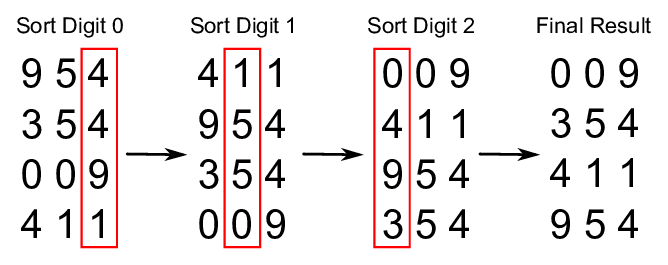
\includegraphics[width=0.8\textwidth]{img/radix.png}
    \caption{\href{https://velog.velcdn.com/images/shitaikoto/post/cc26c311-7ca9-4235-b134-27fc6480b3e9/radix.png}{Radix Sort Algorithm Diagram}}
\end{figure}

\subsubsection{Mã giả}
 
\begin{algorithm}[H]
\caption{Radix Sort}
\label{alg:radix-sort}
\begin{algorithmic}

\Require $A$ is an array of size $n$
\Function {radix-sort}{\textit{A}}
\State $max \gets$ Maximum value in $A$
\State $exp \gets 1$
\While{$max/exp > 0$}
    \Call{counting-sort}{A, exp}
    \State $exp \gets exp \times 10$
\EndWhile
\EndFunction

\Function {counting-sort}{\textit{A}, \textit{exp}}
\State Perform Counting Sort on $A$ based on the digit at $exp$ position
\EndFunction

\end{algorithmic}
\end{algorithm}


\subsubsection{Độ phức tạp}

\textbf{Độ phức tạp thời gian}

Trong cả ba trường hợp (tốt nhất, trung bình, tệ nhất), Radix sort đều cần thực hiện d bước (với d là số chữ số của số lớn nhất trong mảng). Trong mỗi bước, Counting Sort có độ phức tạp thời gian là $O(n)$. Do đó, độ phức tạp thời gian của Radix sort là $O(dn)$.

\textbf{Độ phức tạp không gian}

Radix Sort sử dụng Counting Sort trong mỗi lượt duyệt, do đó sử dụng mảng phụ để lưu kết quả, dẫn đến độ phức tạp thời gian là $O(n)$.

\subsubsection{Nhận xét}

\textbf{Tính ổn định}

Tính ổn định của Radix Sort được đảm bảo bởi cách thức hoạt động của thuật toán. Bằng cách phân nhóm các phần tử dựa trên từng chữ số và giữ nguyên thứ tự tương đối của các phần tử trong mỗi nhóm, Radix Sort đảm bảo rằng thứ tự ban đầu của các phần tử bằng nhau sẽ không bị thay đổi sau khi sắp xếp.

\textbf{Cải tiến}

Binary MSD RadixSort là một biến thể của thuật toán sắp xếp Radix Sort, được tối ưu hóa cho việc sắp xếp các số nguyên. Thuật toán này phân chia các số dựa trên từng chữ số ở cơ số 2 (hệ nhị phân) và không tốn
thêm bộ nhớ làm mảng tạm.
\subsection{Flash Sort}

\subsubsection{Ý tưởng}

Flash Sort là một thuật toán sắp xếp không dựa trên so sánh các phần tử. Nó dựa trên sự phân bố của dữ liệu, tương tự như Counting Sort nhưng có thể áp dụng cho dữ liệu số thực. Flash Sort kết hợp ý tưởng phân hoạch của Counting Sort để chia dữ liệu thành các lớp, sau đó sử dụng Insertion Sort để sắp xếp nội bộ mỗi lớp. Thuật toán có 3 giai đoạn chính:

\begin{itemize}
    \item Phân lớp: Chia dữ liệu thành các lớp dựa trên giá trị của phần tử.
    \item Phân hoạch và hoán vị: Đưa các phần tử vào đúng lớp của chúng.
    \item Sắp xếp nội bộ: Sử dụng Insertion Sort để sắp xếp các phần tử trong mỗi lớp.
\end{itemize}



\subsubsection{Các bước hoạt động}
Chúng ta sẽ thực hiện thuật toán Flash Sort trên mảng:  
\[
A = \{5, 9, 0, 3, 7\}
\]

Bước 1: Tính \textit{min} và \textit{max}
\[
\text{min} = 0, \quad \text{max} = 9
\]

Bước 2: Tạo các nhóm (class). Chọn số lượng nhóm, \( m = 3 \).  
Chỉ số nhóm \( k \) được tính theo công thức:
\[
k = \left\lfloor m \cdot \frac{A[i] - \text{min}}{\text{max} - \text{min}} \right\rfloor
\]
với \( m = 3 \), \( \text{min} = 0 \), và \( \text{max} = 9 \).

Bước 3: Gán các phần tử vào nhóm. Tính chỉ số nhóm \( k \) cho từng phần tử trong \( A \):

\[
\begin{array}{|c|c|}
\hline
\text{Phần tử } (A[i]) & \text{Chỉ số nhóm } (k) \\
\hline
5 &  1 \\
9 &  2 \\
0 &  0 \\
3 &  1 \\
7 &  2 \\
\hline
\end{array}
\]

Phân phối các nhóm:
\[
\text{Nhóm 0: } \{0\}, \quad \text{Nhóm 1: } \{5, 3\}, \quad \text{Nhóm 2: } \{9, 7\}
\]

Bước 4: Sắp xếp lại các phần tử
Sắp xếp lại \( A \) bằng cách nhóm các phần tử vào từng nhóm:
\[
A = \{0, 5, 3, 9, 7\}
\]

Bước 5: Sắp xếp chèn trong từng nhóm
\begin{itemize}
    \item Nhóm 0: \(\{0\}\) đã được sắp xếp.  
    \item Nhóm 1: \(\{5, 3\}\):  
  Thực hiện sắp xếp chèn:
  \[
  \{5, 3\} \to \{3, 5\}
  \]
    \item Nhóm 2: \(\{9, 7\}\):  
  Thực hiện sắp xếp chèn:
  \[
  \{9, 7\} \to \{7, 9\}
  \]
\end{itemize}

Bước 6: Kết hợp các nhóm đã sắp xếp
Gộp các nhóm đã được sắp xếp để có mảng kết quả cuối cùng:
\[
A = \{0, 3, 5, 7, 9\}
\]


\subsubsection{Mã giả}


 
\begin{algorithm}[H]
\caption{Flash Sort}
\label{alg:flash-sort}
\begin{algorithmic}


\Require $A$ is an array of size $n$
\Function {flash-sort}{\textit{A}, \textit{n}}
    \State Compute $min$ and $max$ of $A$
    \If{$min = max$}
        \State \Return $A$ \Comment{All elements are identical; array is sorted}
    \EndIf
    \State Create $m$ classes \Comment{Typically $m = \alpha \cdot n$ where $\alpha \in (0, 1]$ is a constant}
    \State Initialize an array $L$ of size $m$ to store class boundaries
    \For{$i = 0$ to $n-1$}
        \State Compute the class index $k$ for $A[i]$:
       $$k = \left\lfloor m \cdot \frac{A[i] - min}{max - min} \right\rfloor$$
        \State Assign $A[i]$ to class $k$ and update $L[k]$
    \EndFor
    \State Rearrange elements of $A$ such that elements in each class are grouped together
    \For{each class $k$ in $L$}
        \State Perform Insertion Sort on elements in class $k$
    \EndFor
    \State \Return $A$
\EndFunction


\end{algorithmic}
\end{algorithm}


\subsubsection{Độ phức tạp}


\textbf{Độ phức tạp thời gian}

Phân tích các bước trong thuật toán:
\begin{itemize}
    \item Bước phân lớp có độ phức tạp thời gian: \( O(n) \).
\item Bước hoán vị cũng có độ phức tạp thời gian: \( O(n) \).
\item Trong mỗi nhóm, thuật toán sử dụng sắp xếp chèn (Insertion Sort). Nếu mỗi nhóm chứa khoảng \( \frac{n}{m} \) phần tử, chi phí tổng cộng cho bước này là:
\[
O\left( m \cdot \left(\frac{n}{m}\right)^2 \right) = O\left(\frac{n^2}{m}\right).
\]
\end{itemize}

Khi \( m = \alpha n \) (\( \alpha \) là một hằng số), độ phức tạp trở thành \( O(n) \).

Do đó, độ phức tạp thời gian tổng cộng của thuật toán Flash Sort là \( O(n) \) cho các dữ liệu phân bố đồng đều, nhưng có thể giảm hiệu năng xuống \( O(n^2) \) với các phân bố dữ liệu không đồng đều.

\textbf{Độ phức tạp không gian}

Thuật toán cần thêm bộ nhớ để lưu ranh giới các nhóm hoặc số lượng phần tử trong mỗi nhóm. Do đó, độ phức tạp không gian là \( O(n) \).

\subsubsection{Nhận xét}
Flash Sort là thuật toán tốt đối với các mảng lớn có dữ liệu phân bố đồng đều và hiệu quả vượt trội so với nhiều thuật toán \( O(n \log n) \) (như Quicksort) trong các trường hợp thực tế. Tuy nhiên, hiệu năng của Flash Sort phụ thuộc nhiều vào phân bố dữ liệu. Hiệu quả kém đối với các phân bố không đồng đều. Cần tính toán trước \( \text{min} \) và \( \text{max} \), đồng thời cần lựa chọn số lượng nhóm \( m \) một cách phù hợp.


\textbf{Cải tiến} 

Flash Sort tỏ ra không hiệu quả ở trường hợp tệ nhất khi tất cả các phần tử đều vào 1 lớp, cũng như thứ tự bị đảo ngược. Khi đó có thể thay thế một thuật toán khác như Merge Sort thể thay thế Insertion Sort trong trường hợp này.


\section{Kết quả thực nghiệm và biểu đồ}

Lưu ý: Hai thuật toán Bubble Sort, Shaker Sort trong thực nghiệm này đều có biến cờ hiệu để dừng sớm khi đã sắp xếp xong. 

\subsection{Kết quả thực nghiệm} \label{subsec:experimental_result}
Các bảng \ref{tab:randomize_10000_30000_50000}, \ref{tab:randomize_100000_300000_500000}, \ref{tab:nearly_sorted_10000_30000_50000}, \ref{tab:nearly_sorted_100000_300000_500000}, \ref{tab:sorted_10000_30000_50000}, \ref{tab:sorted_100000_300000_500000}, \ref{tab:reversed_10000_30000_50000}, \ref{tab:reversed_100000_300000_500000} là kết quả thực nghiệm cho 11 thuật toán đã được giới thiệu trên các bộ dữ liệu khác nhau.

\input{./experimental_result/result_tables.tex}

11 thuật toán được phân loại thành ba nhóm như sau để thuận tiện cho việc gọi tên: 
\begin{itemize}
    \item Thuật toán cơ bản (Selection Sort, Insertion Sort, Bubble Sort, Shaker Sort)
    \item Thuật toán cải tiến (Shell Sort, Heap Sort, Merge Sort, Quick Sort)
    \item Thuật toán không so sánh (Counting Sort, Radix Sort, Flash Sort)
\end{itemize}

\subsubsection{Biểu đồ thời gian chạy}

\textbf{3.2.1.1. Dữ liệu ngẫu nhiên}

Từ hình \ref{fig:randomize_running_time}, dễ thấy các thuật toán cơ bản có thời gian chạy lớn hơn rất nhiều so với các thuật toán còn lại. Bubble Sort có thời gian chạy chậm nhất (đường màu xanh). Shaker Sort là phiên bản cải tiến của Bubble Sort, có thời gian chạy tương đối tốt hơn Bubble Sort một chút. 4 thuật toán này có thời gian chạy tăng mạnh khi kích thước dữ liệu lớn hơn (bộ dữ liệu lên đến 500.000 phần tử). Điều này phù hợp với độ phức tạp $O(n^2)$ của chúng.


Các thuật còn lại bao gồm Shell Sort, Heap Sort, Merge Sort, Quick Sort, Counting Sort, Radix Sort, Flash Sort do thời gian chạy nhỏ nên các đường biểu diễn của chúng bị đè lên nhau thành một đường duy nhất (đường màu đỏ tía). Tiến hành loại bỏ 4 thuật toán cơ bản có thời gian chạy lớn, được hình \ref{fig:randomize_running_time_filtered}.

\begin{figure}[H]
    \centering
    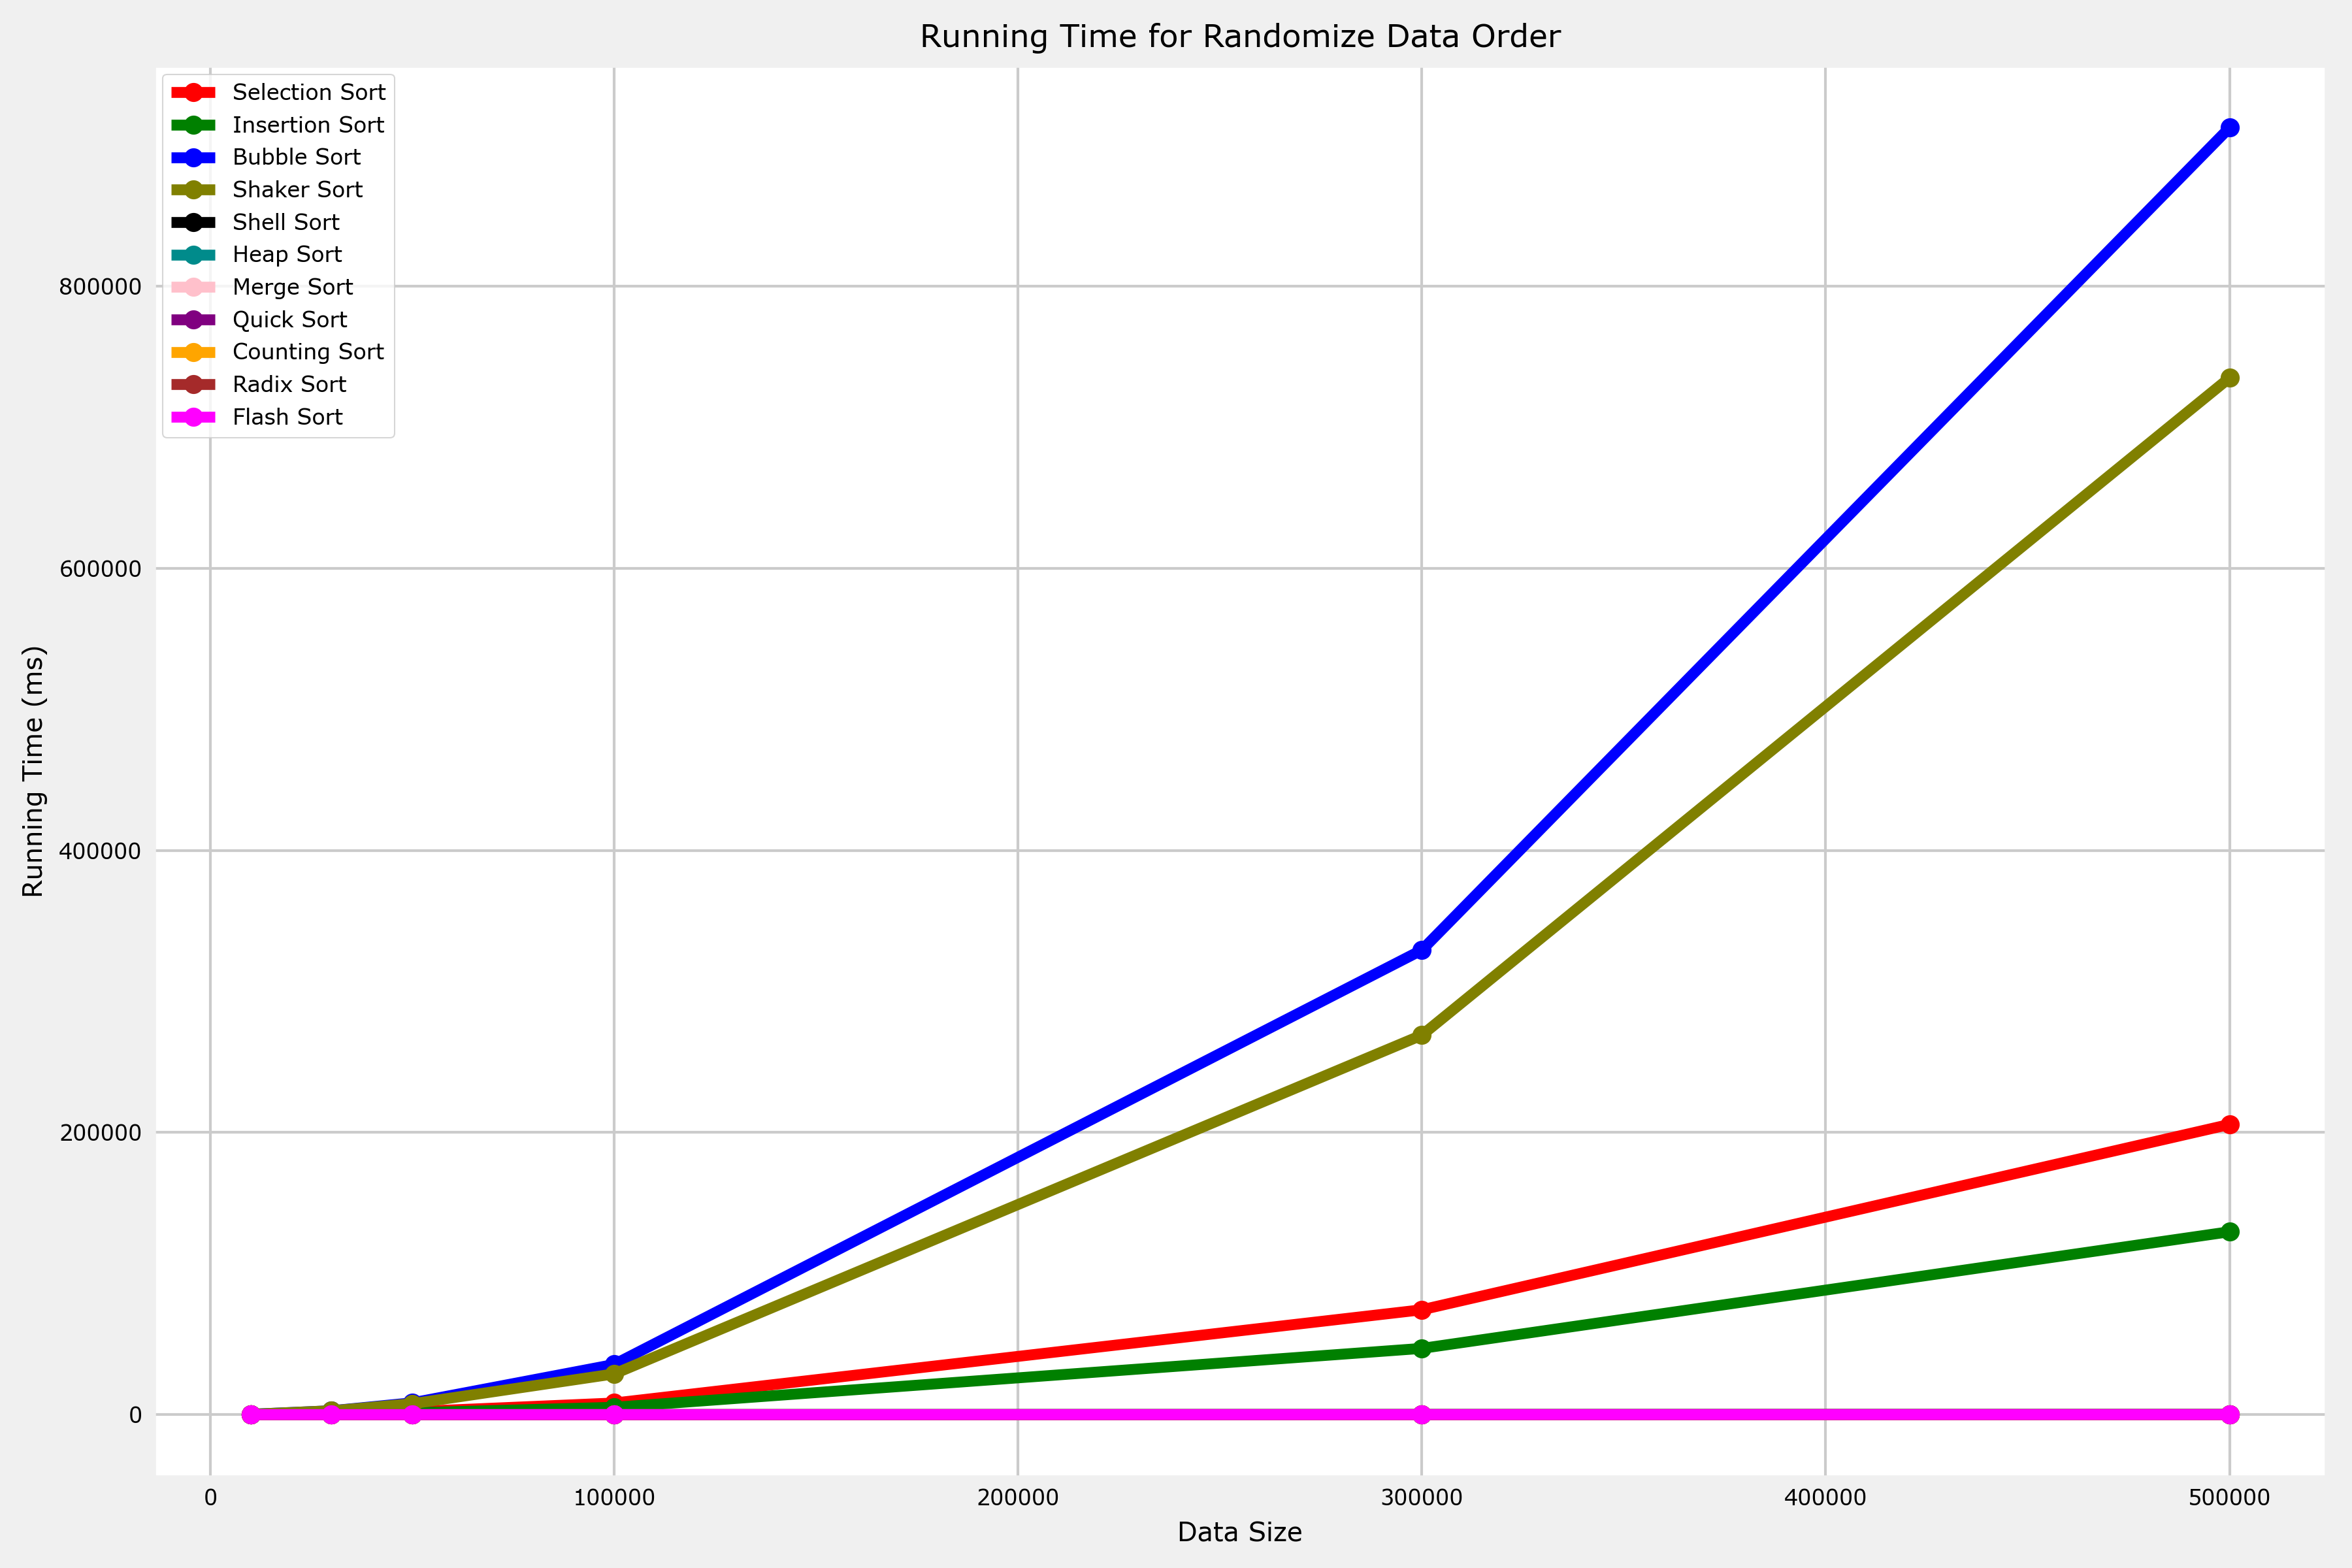
\includegraphics[width=\textwidth]{experimental_result/images/randomize_running_time.png}
    \caption{Thời gian chạy của 11 thuật toán với dữ liệu ngẫu nhiên}
    \label{fig:randomize_running_time}
\end{figure}


\begin{figure}[H]
    \centering
    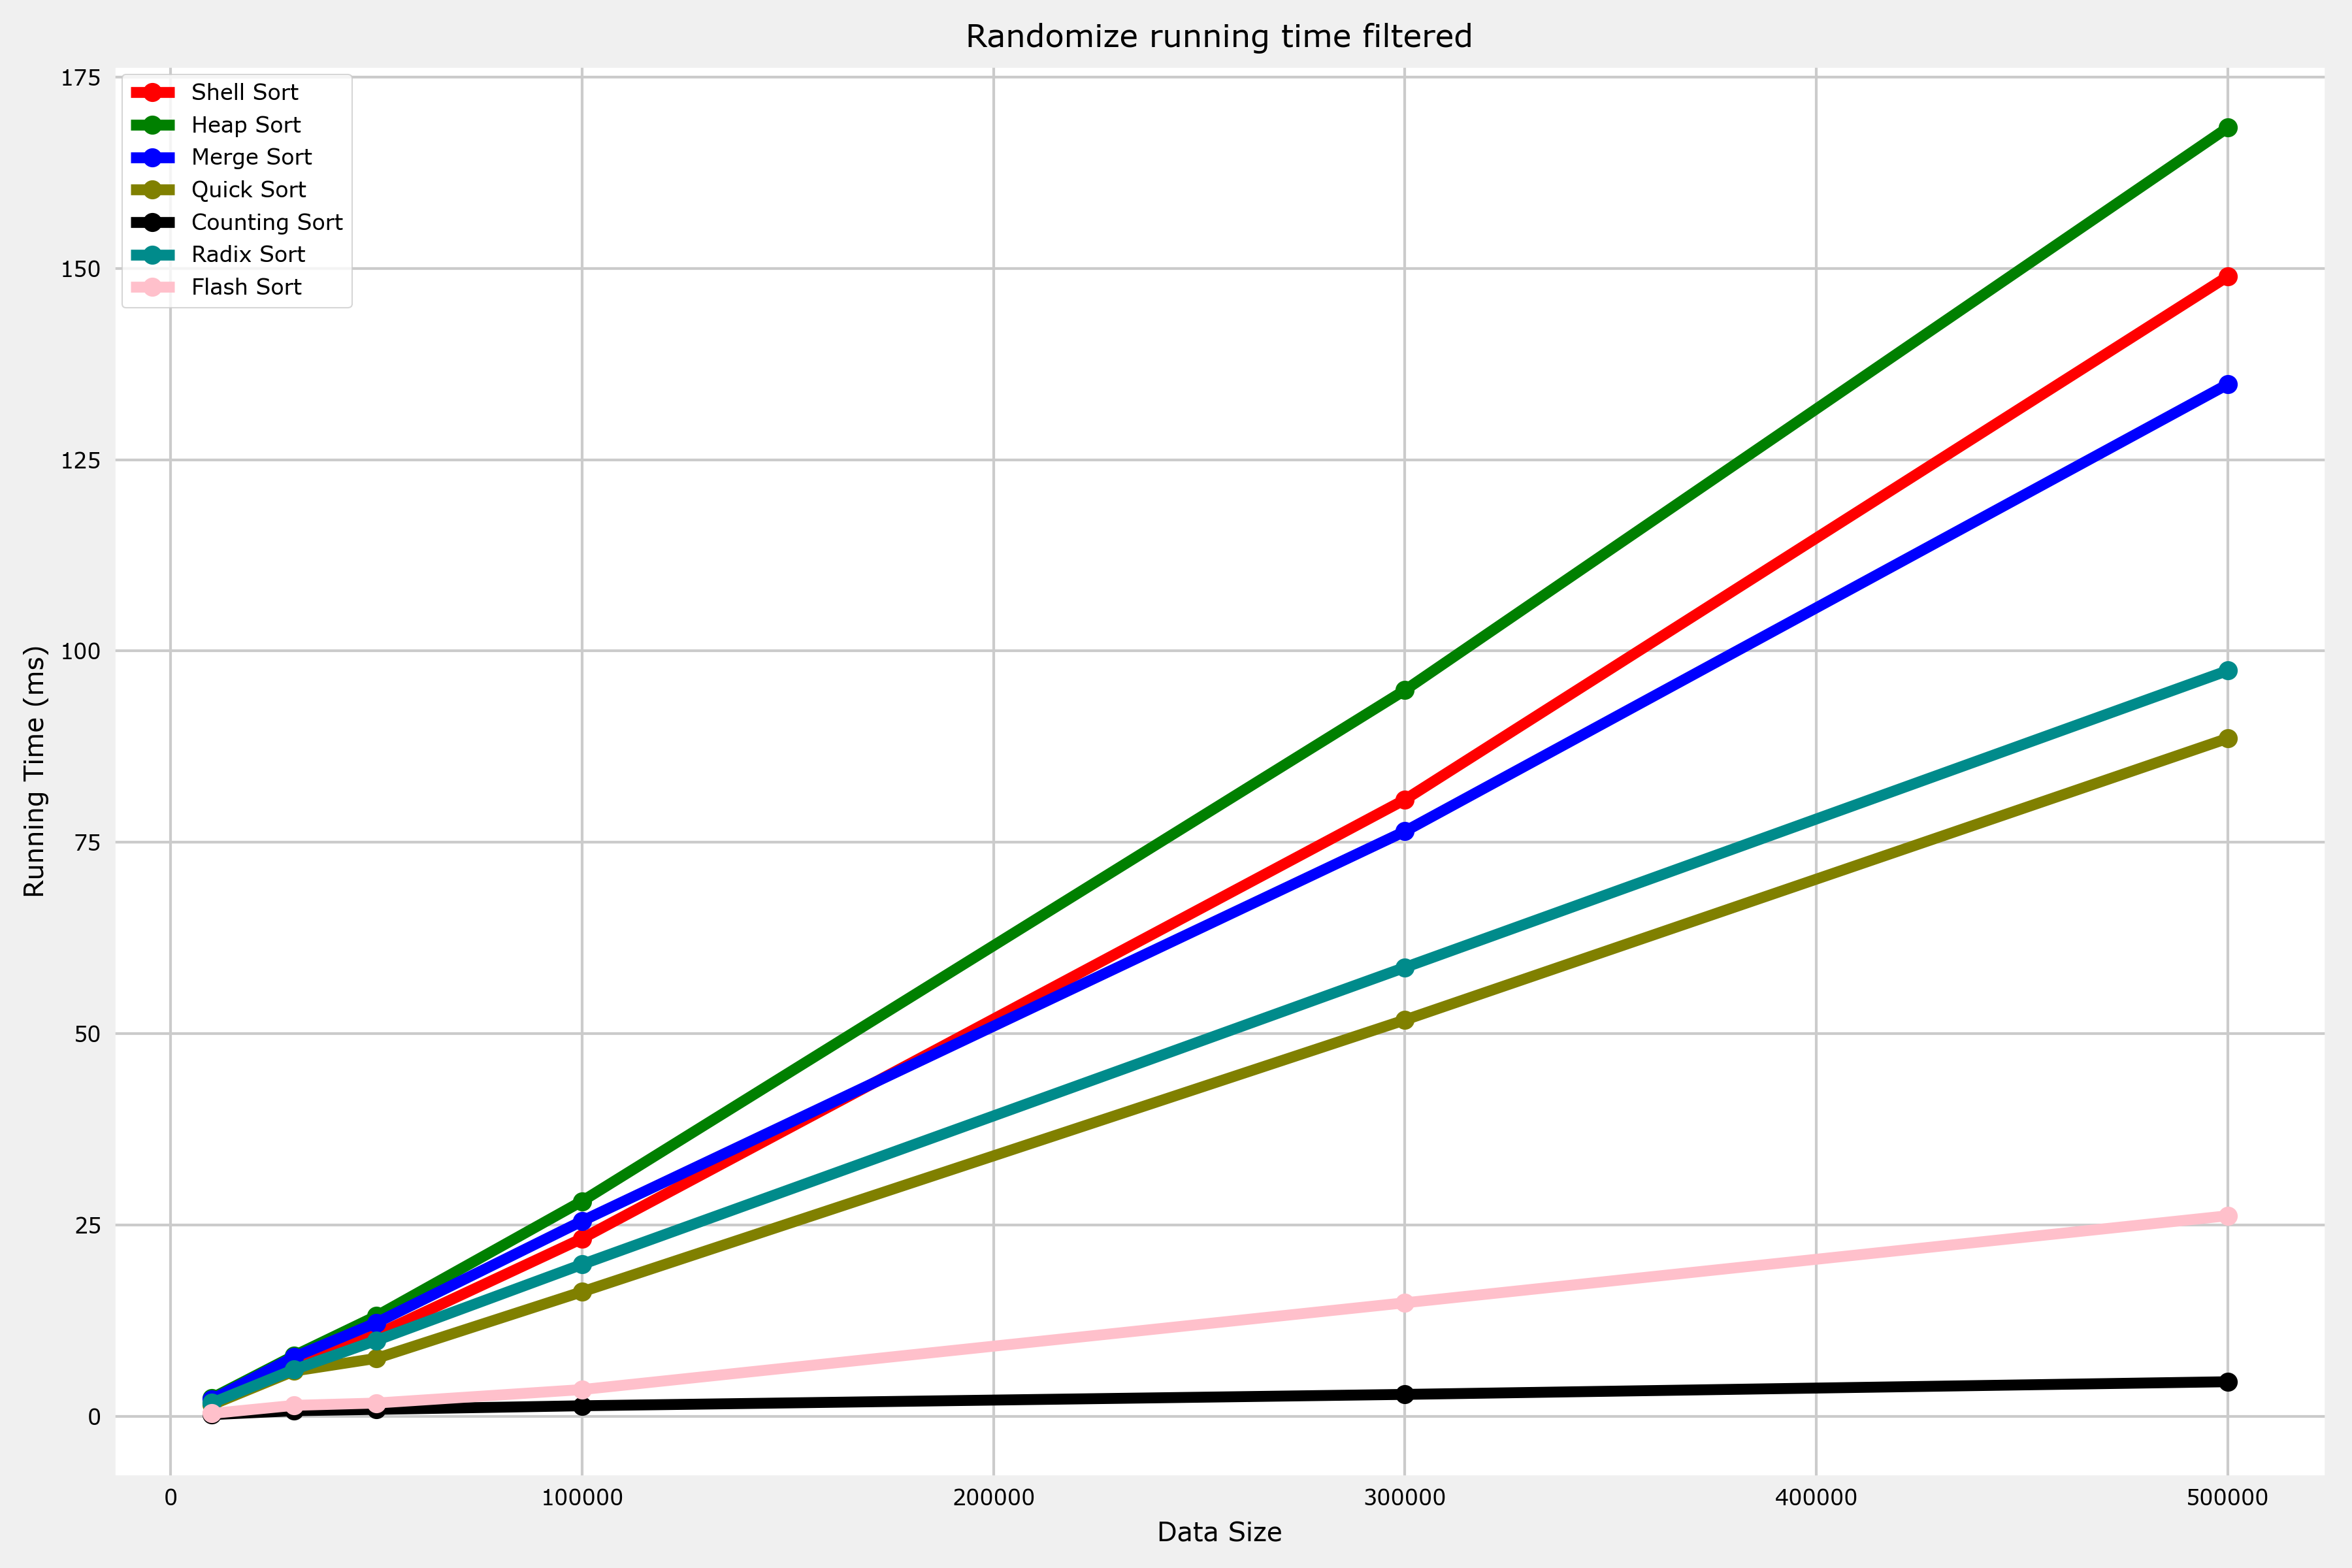
\includegraphics[width=\textwidth]{experimental_result/images/randomize_running_time_filtered.png}
    \caption{Thời gian chạy của 11 thuật toán với dữ liệu ngẫu nhiên sau khi loại bỏ outlier}
    \label{fig:randomize_running_time_filtered}
\end{figure}

Các thuật toán này có xu hướng tuyến tính hơn so với nhóm trước. Thuật toán Counting Sort và Flash Sort là hai thuật toán nhanh nhất, trong khi nhóm các thuật toán cải tiến có thời gian chạy cao hơn nhưng vẫn ổn định. Đặc biệt, Counting Sort có thời gian chạy rất nhỏ các tất cả trường hợp, đều bé hơn $5 ms$ (đường màu đen nằm rất gần trục hoành).




\begin{figure}[H]
    \centering
    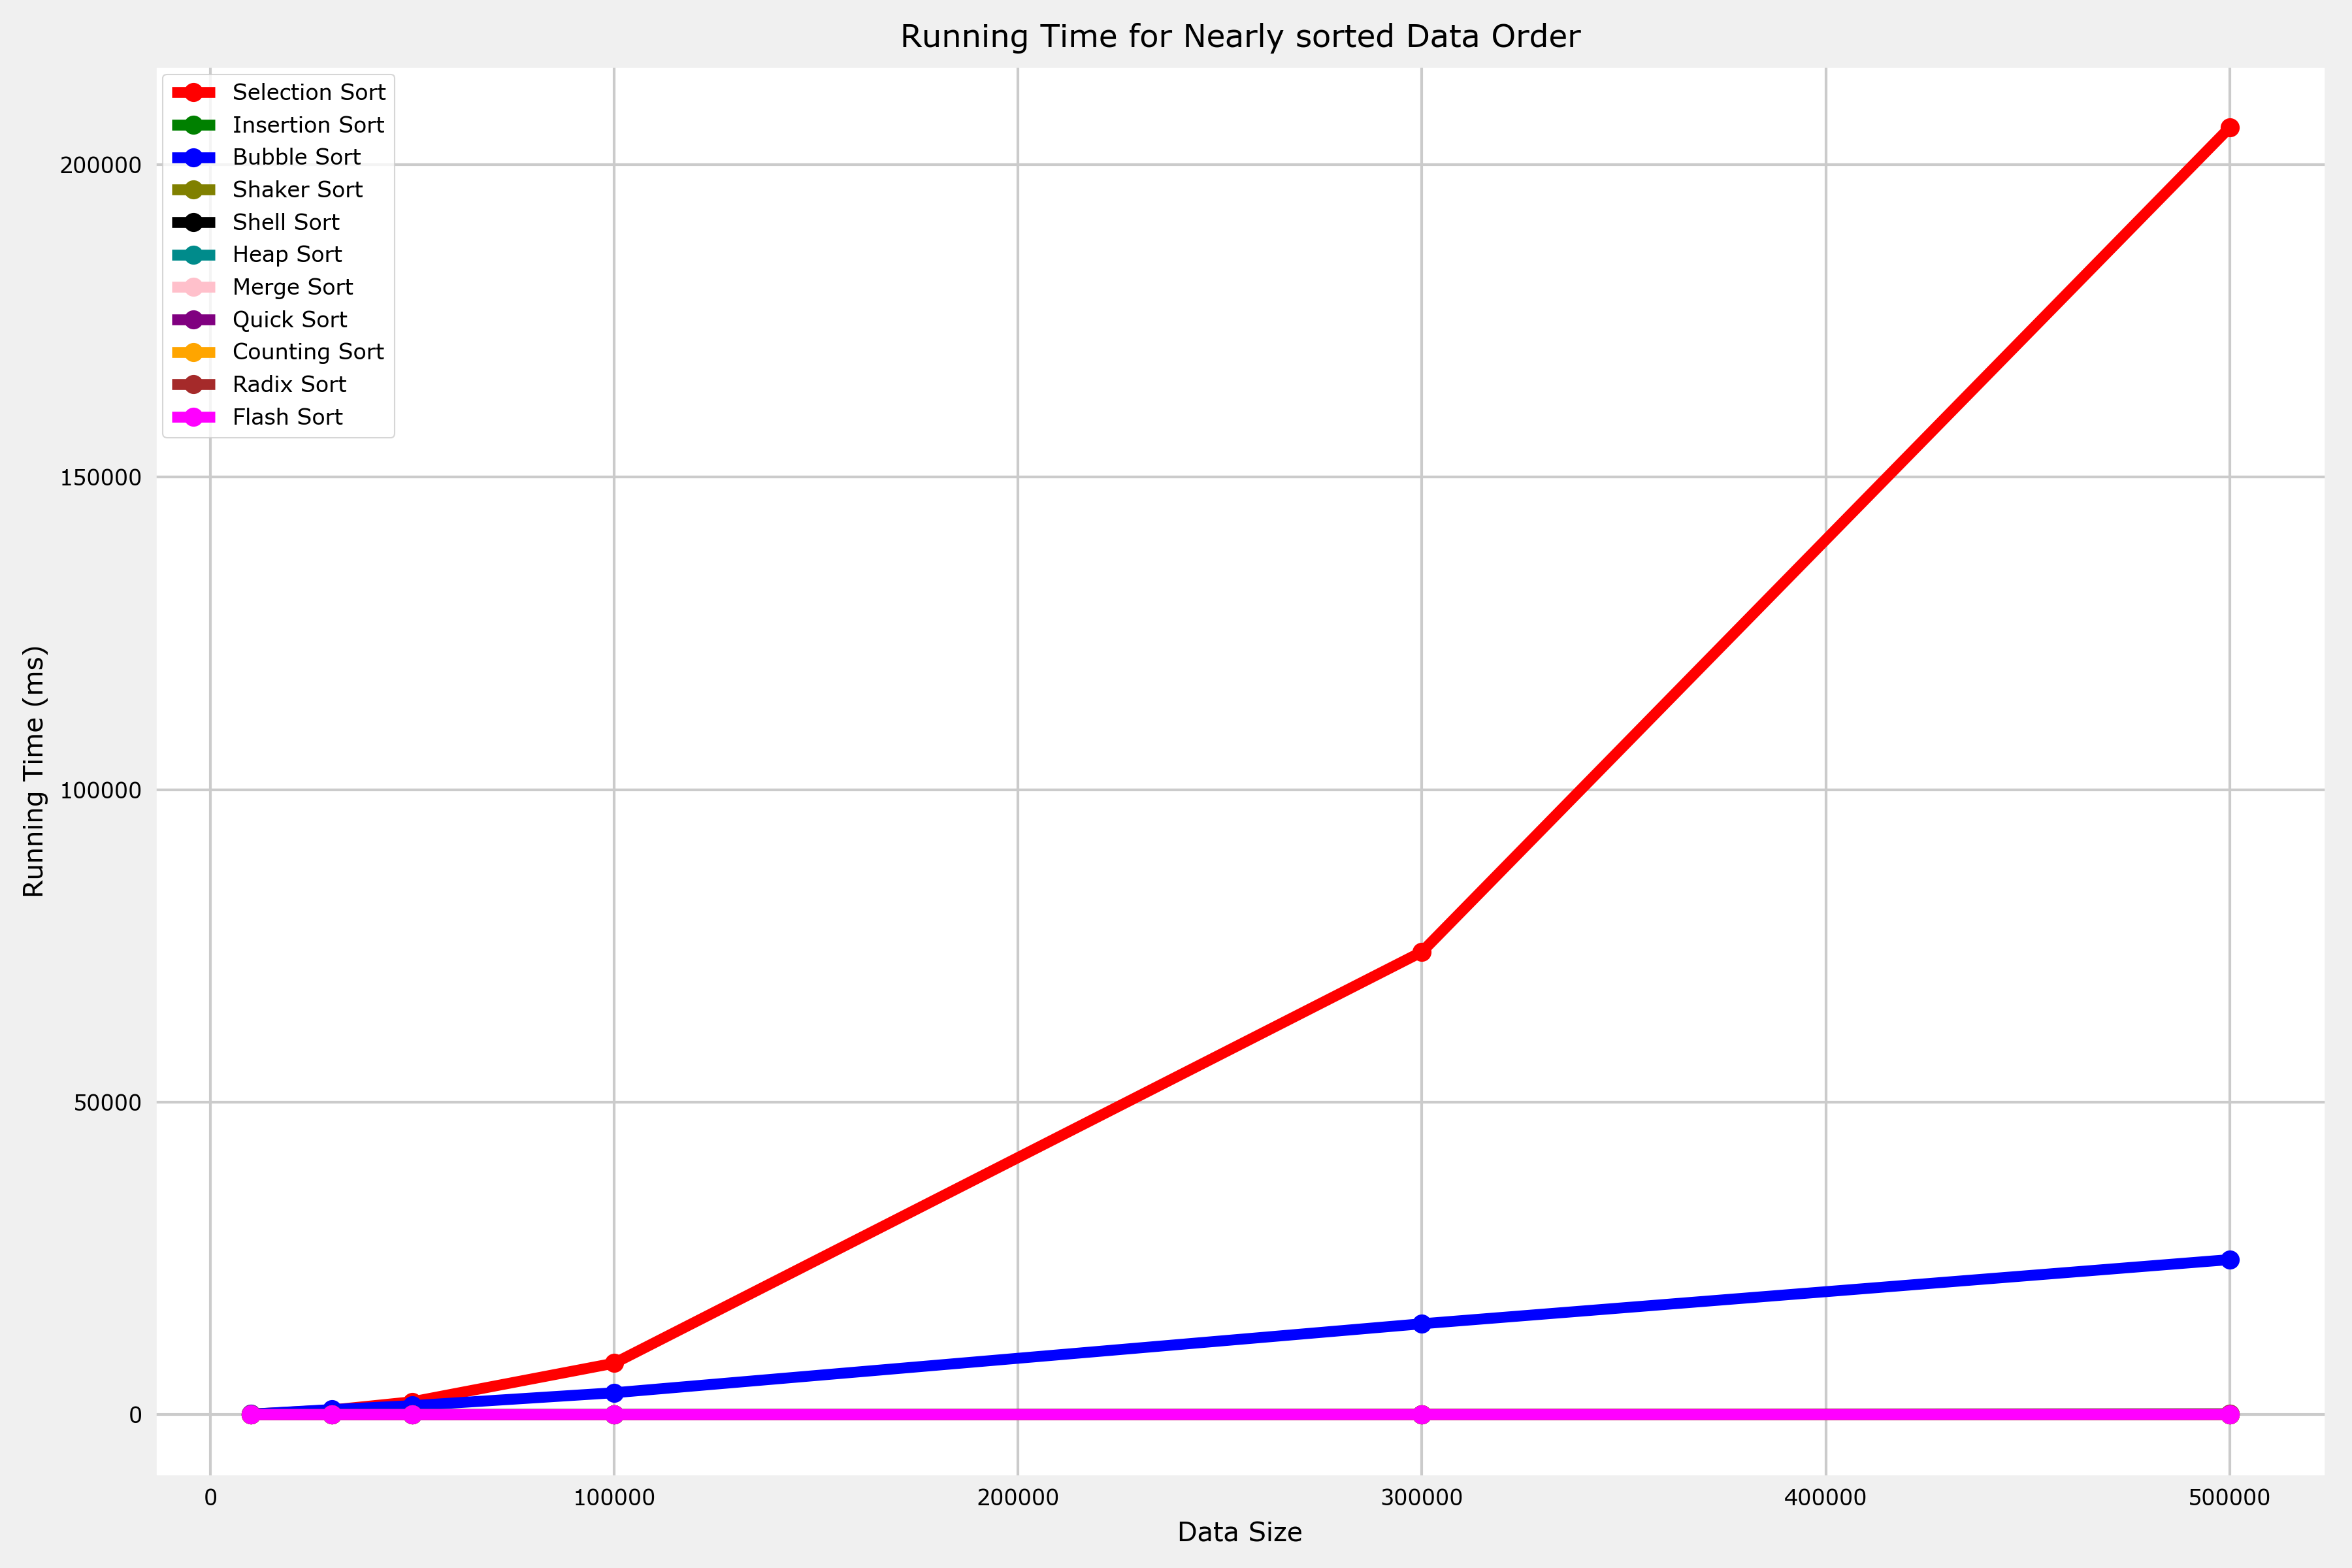
\includegraphics[width=\textwidth]{experimental_result/images/nearly_sorted_running_time.png}
    \caption{Thời gian chạy của 11 thuật toán với dữ liệu gần sắp xếp hoàn chỉnh}
    \label{fig:nearly_sorted_running_time}
\end{figure}
\textbf{3.2.1.2. Dữ liệu gần sắp xếp hoàn chỉnh}


Selection Sort có màn thể hiện rất tệ với dữ liệu gần sắp xếp hoàn chỉnh. Hình \ref{fig:nearly_sorted_running_time} thể hiện rõ độ phức tạp $O(n^2)$ của Selection Sort, tăng rất mạnh khi kích thước dữ liệu lên tới 500.000 phần tử. Thời gian chạy của Bubble Sort tốt hơn Selection Sort nhưng vẫn không tốt bằng các thuật toán khác. Các thuật toán còn lại không thể nhìn thấy do thời gian chạy của chúng nhanh hơn rất nhiều so với Selection Sort. Tiến hành loại bỏ Selection Sort và Bubble Sort, kết quả như hình \ref{fig:nearly_sorted_running_time_filtered}.


\begin{figure}[H]
    \centering
    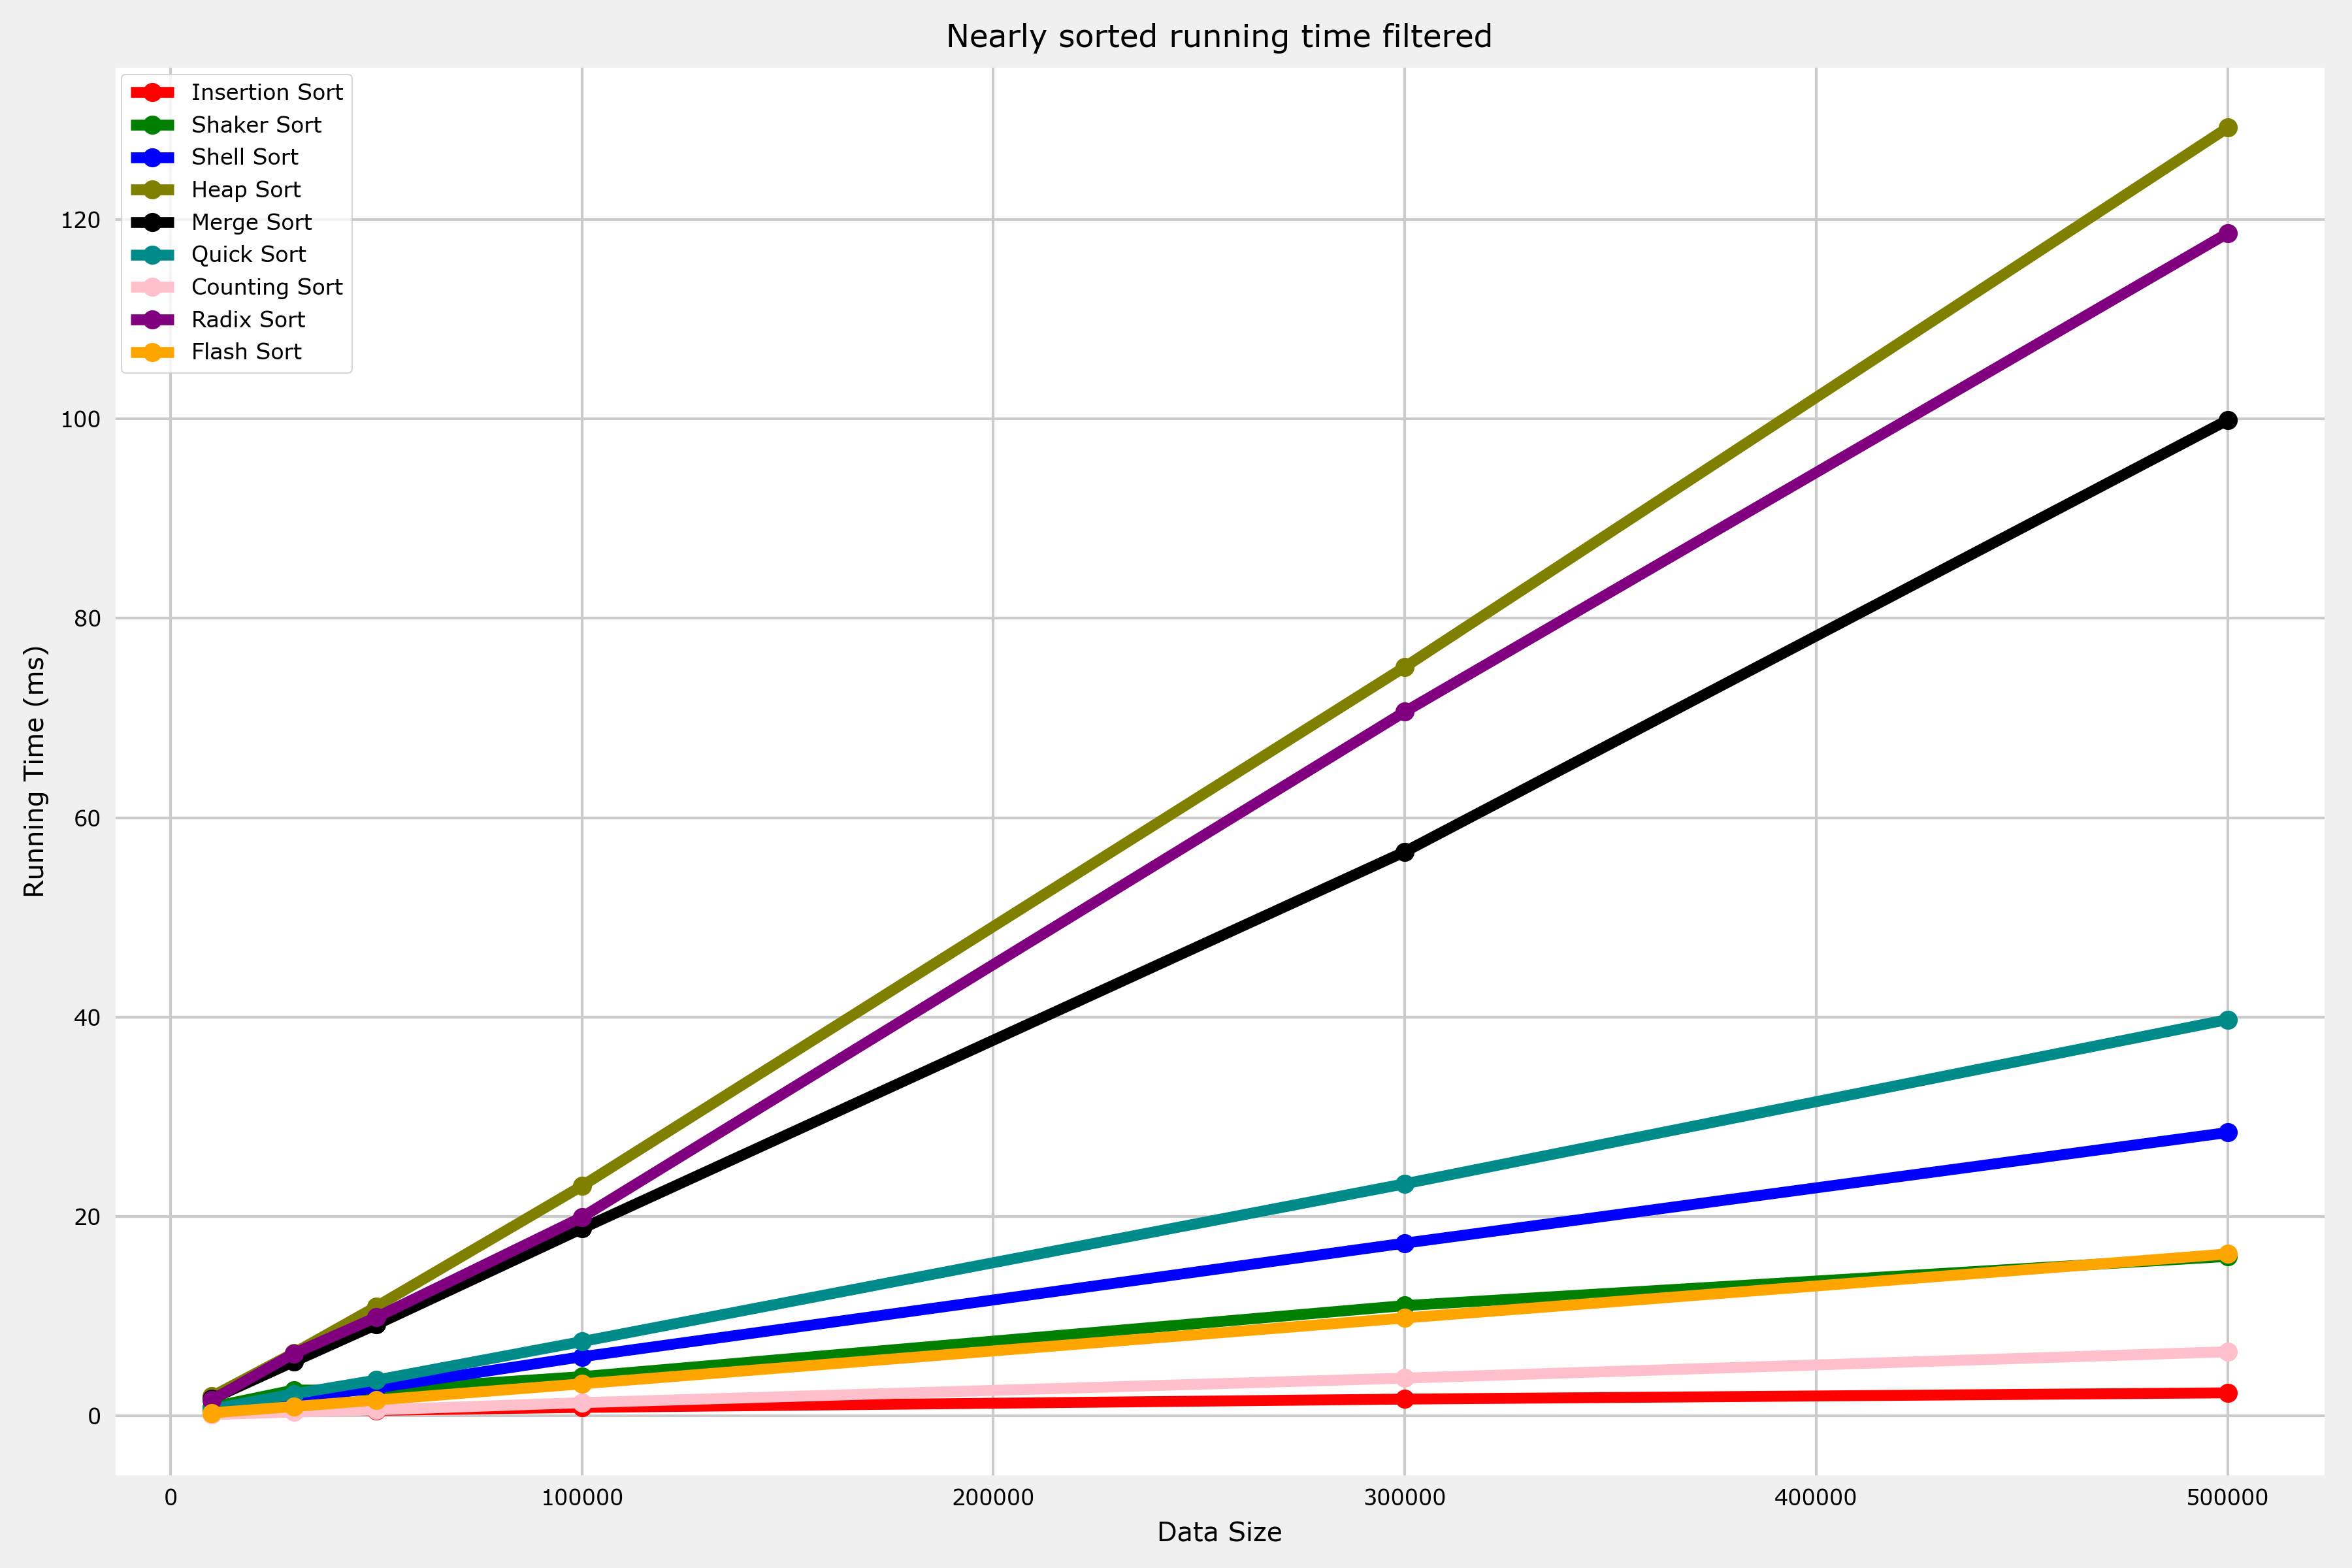
\includegraphics[width=\textwidth]{experimental_result/images/nearly_sorted_running_time_filtered.png}
    \caption{Thời gian chạy của 11 thuật toán với dữ liệu gần sắp xếp hoàn chỉnh sau khi loại bỏ outlier}
    \label{fig:nearly_sorted_running_time_filtered}
\end{figure}

Biểu đồ \ref{fig:nearly_sorted_running_time_filtered} lúc này có xu hướng chia thành hai nhóm nhóm 1 (Heap Sort, Radix Sort, Merge Sort) và nhóm 2, nhanh hơn (Quick Sort, Shell Sort, Shaker Sort, Flash Sort, Counting Sort, Insertion) .Insertion Sort có thời gian thực thi nhanh nhất với bộ dữ liệu này. Điều này khá phù hợp với trường hợp tốt nhất của Insertion Sort là dữ liệu đã sắp xếp. Shaker Sort tốt hơn nhiều so với Bubble Sort và xấp xỉ Flash Sort. Các thuật toán cải tiến và không sắp xếp khá ổn định giống như bộ dữ liệu trước.



\begin{figure}[H]
    \centering
    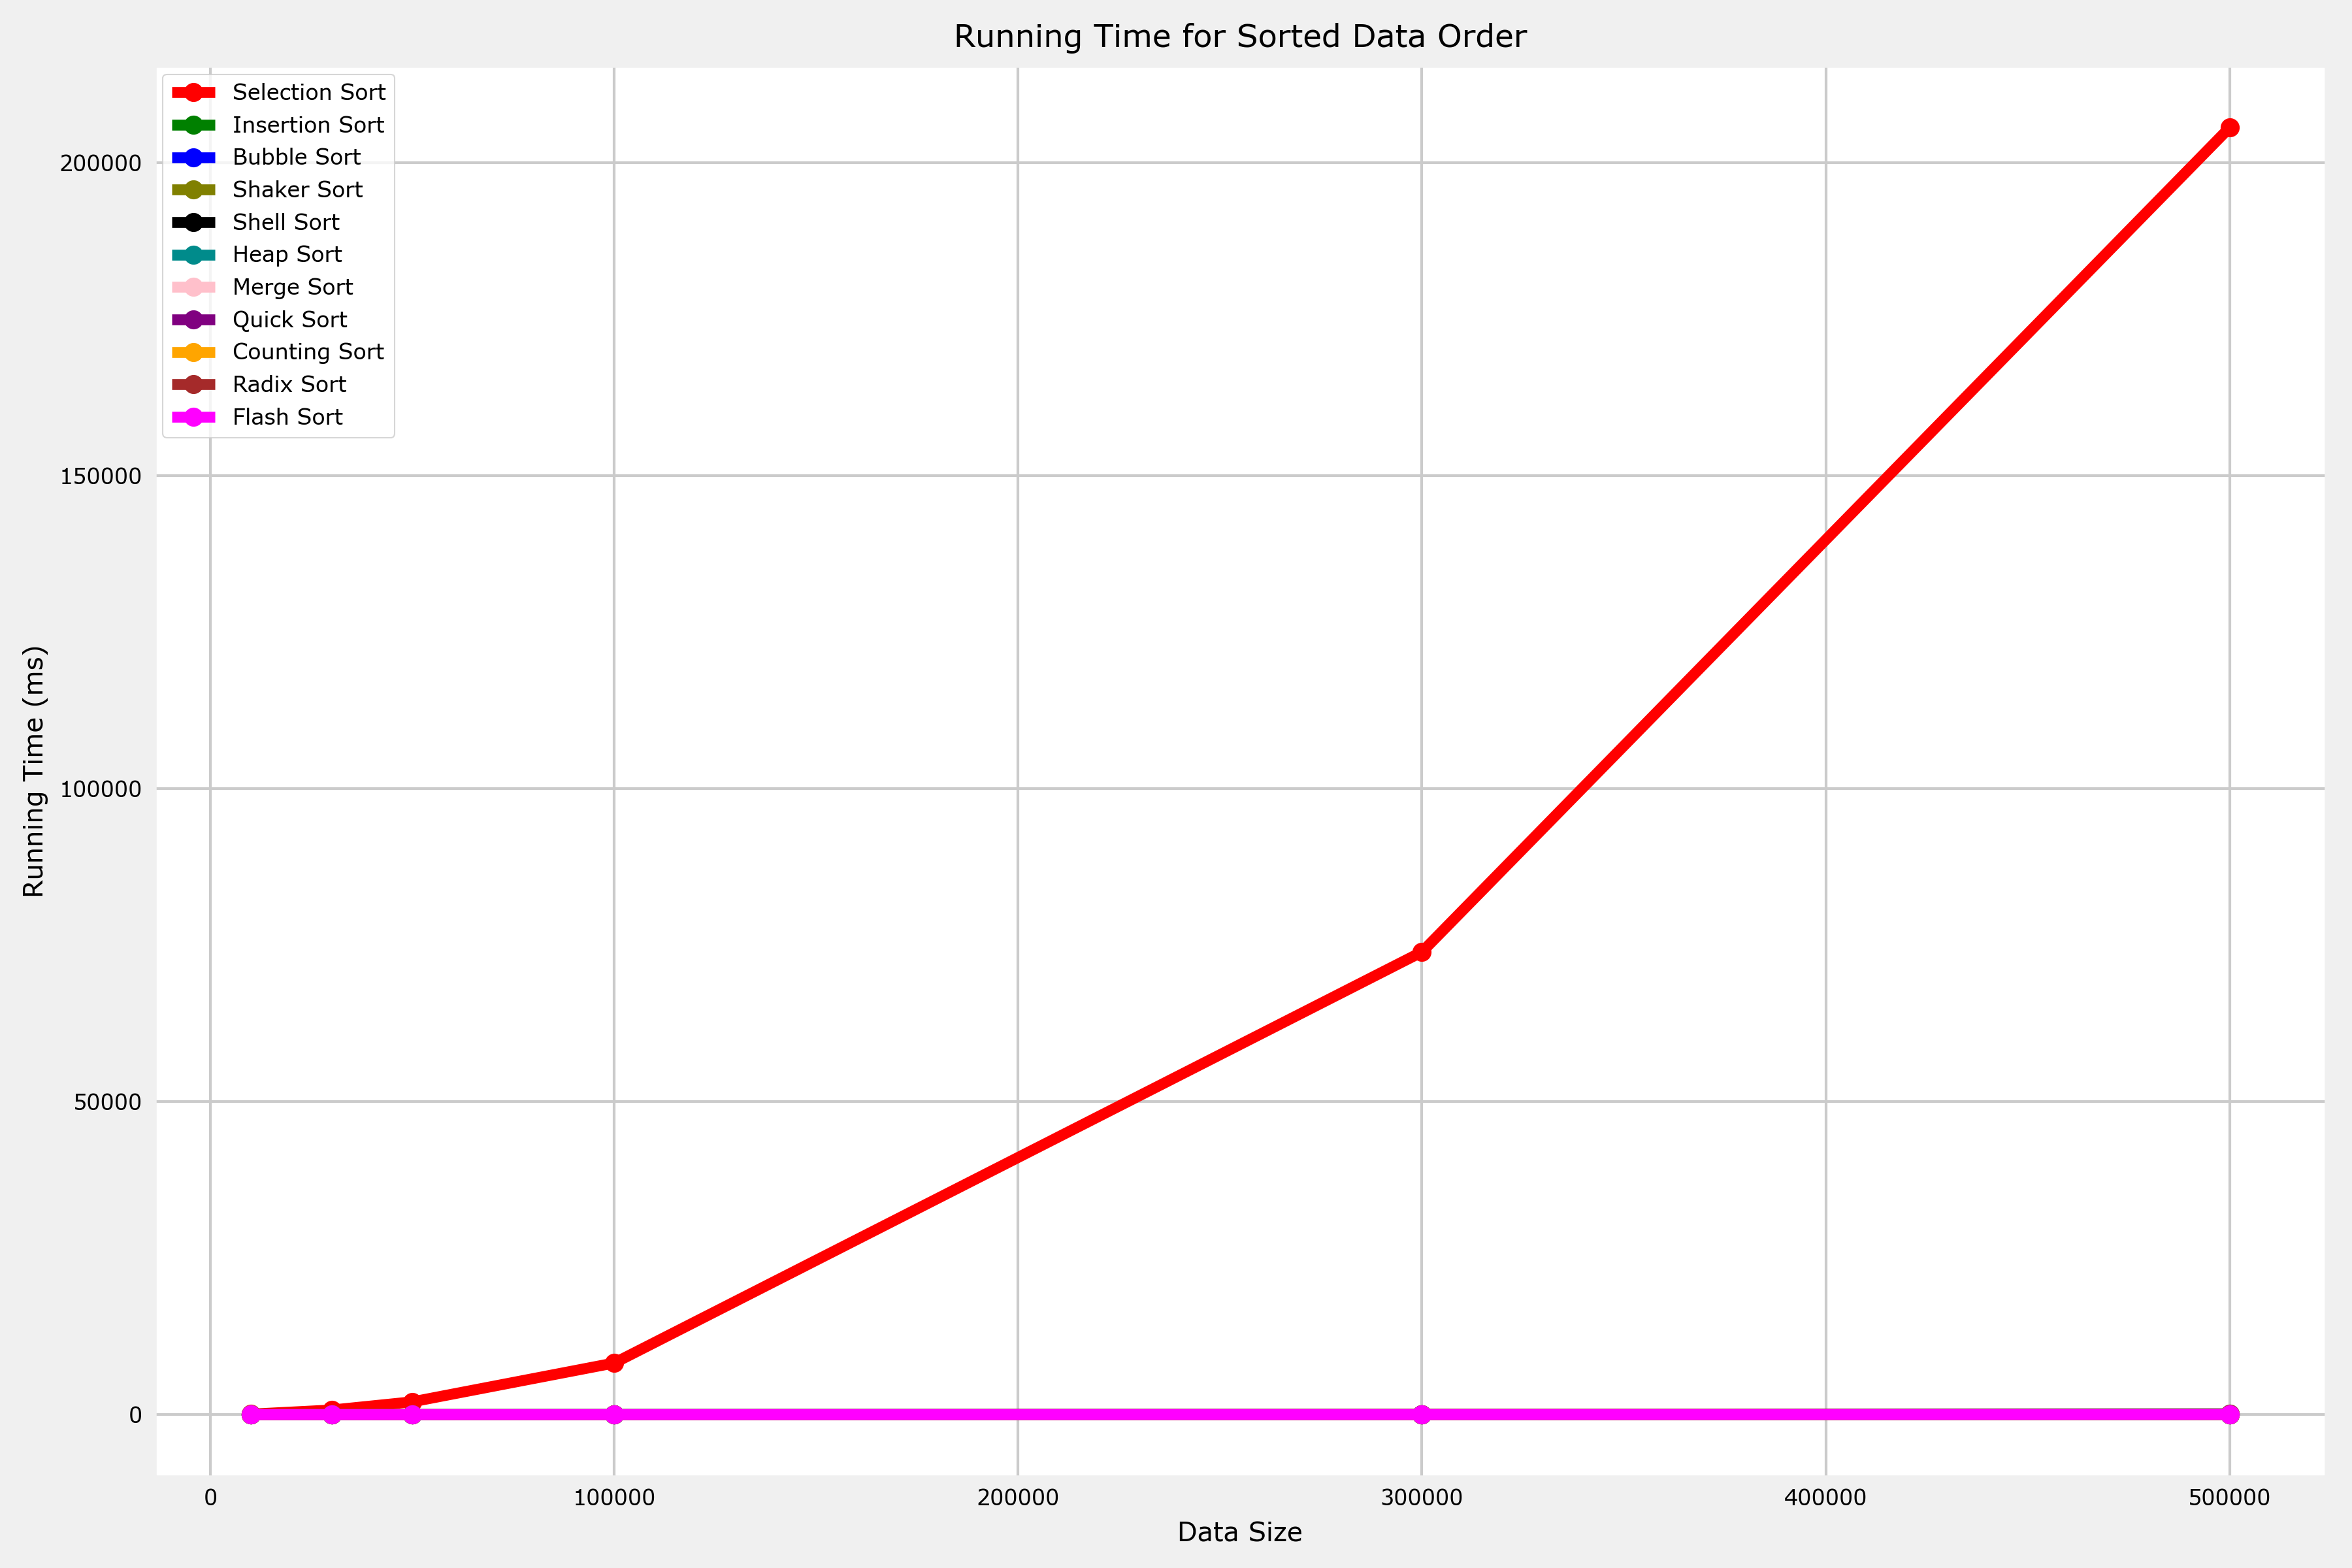
\includegraphics[width=\textwidth]{experimental_result/images/sorted_running_time.png}
    \caption{Thời gian chạy của 11 thuật toán với dữ liệu được sắp xếp}
    \label{fig:sorted_running_time}
\end{figure}

\textbf{3.2.1.3. Dữ liệu được sắp xếp}

Selection vẫn có thời gian thực thi lớn so với các thuật toán còn lại như trên hình \ref{fig:sorted_running_time}. Tiếp tục tách Selection Sort ra khỏi biểu đồ.

\begin{figure}[H]
    \centering
    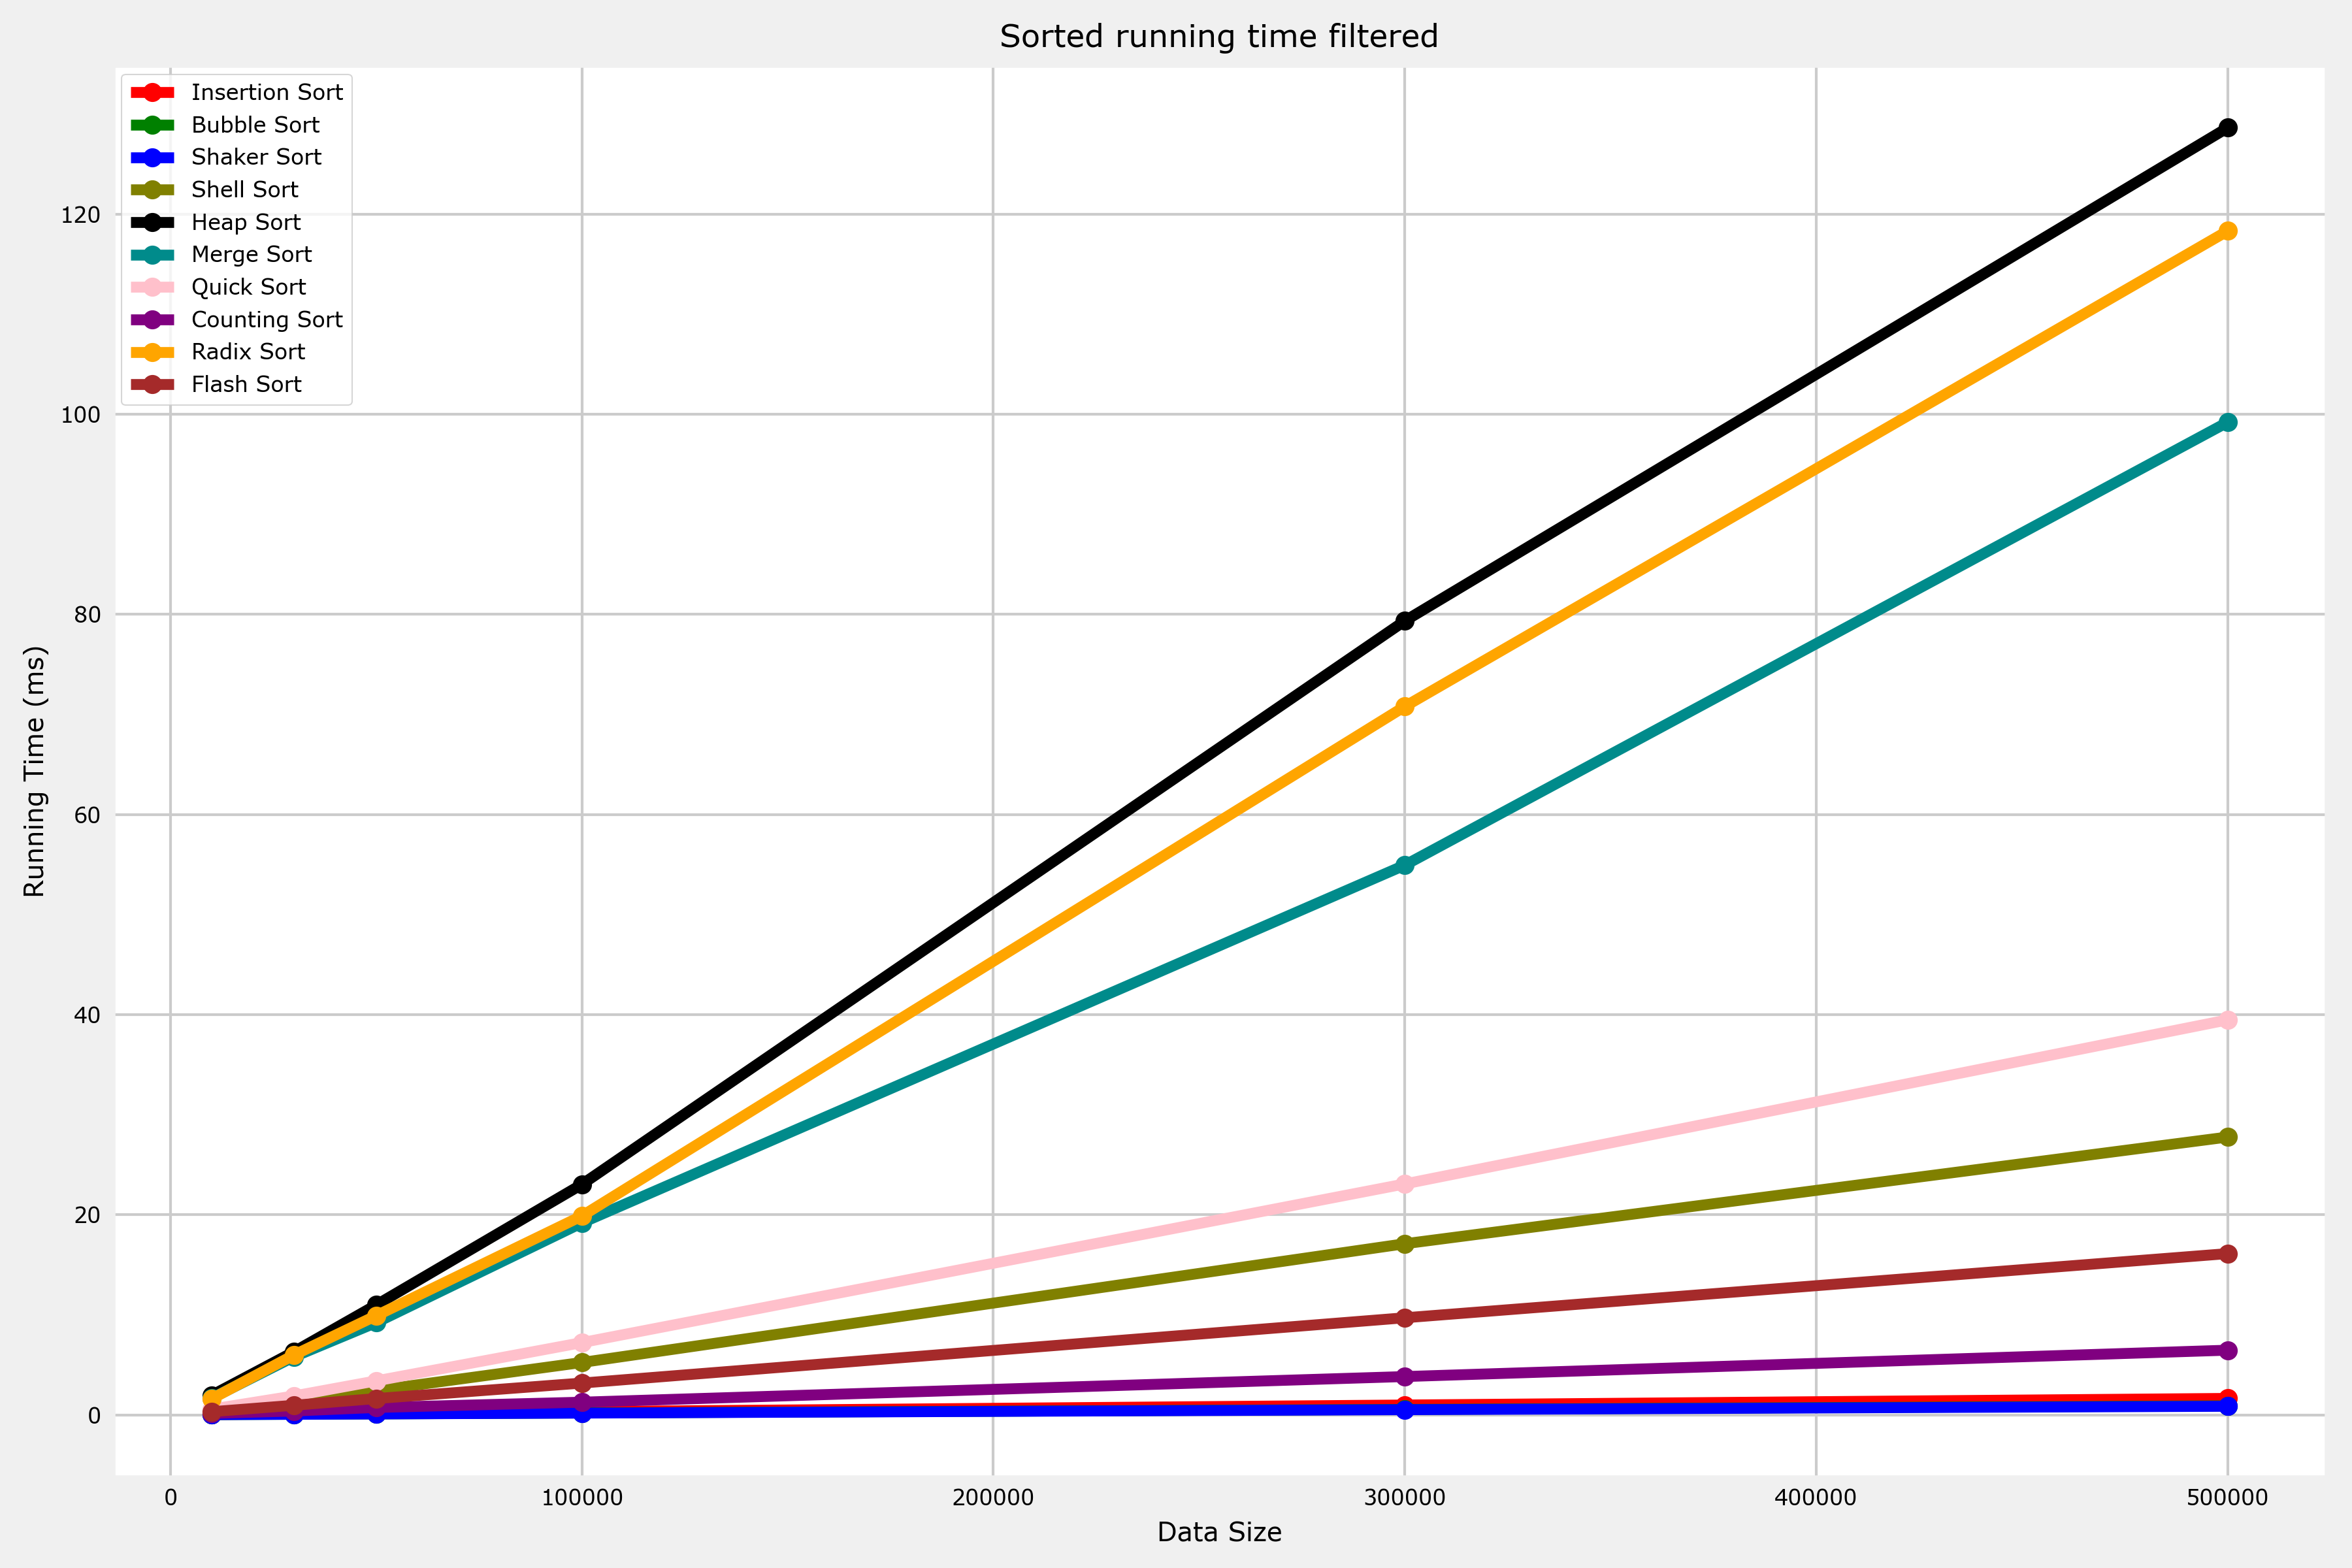
\includegraphics[width=\textwidth]{experimental_result/images/sorted_running_time_filtered.png}
    \caption{Thời gian chạy của 11 thuật toán với dữ liệu được sắp xếp sau khi loại bỏ outlier}
    \label{fig:sorted_running_time_filtered}
\end{figure}

Có hai nhóm thuật toán chính trên biểu đồ \ref{fig:sorted_running_time_filtered}: nhóm 1 (Heap Sort, Radix Sort, Merge Sort) và nhóm 2 (các thuật toán còn lại). Nhóm 1 vẫn giống như trên bộ dữ liệu gần sắp xếp hoàn chỉnh, tương đối ổn định. Nhóm 2 có tốc độ tăng thời gian chạy theo của kích thước của dữ liệu chậm hơn so với nhóm 1. Shaker Sort và Insertion Sort là hai thuật toán nhanh nhất. Bộ dữ liệu này chính là trường hợp tốt nhất cho độ phức tạp thời gian của hai thuật toán này và bằng $\Theta(n)$.


\begin{figure}[H]
    \centering
    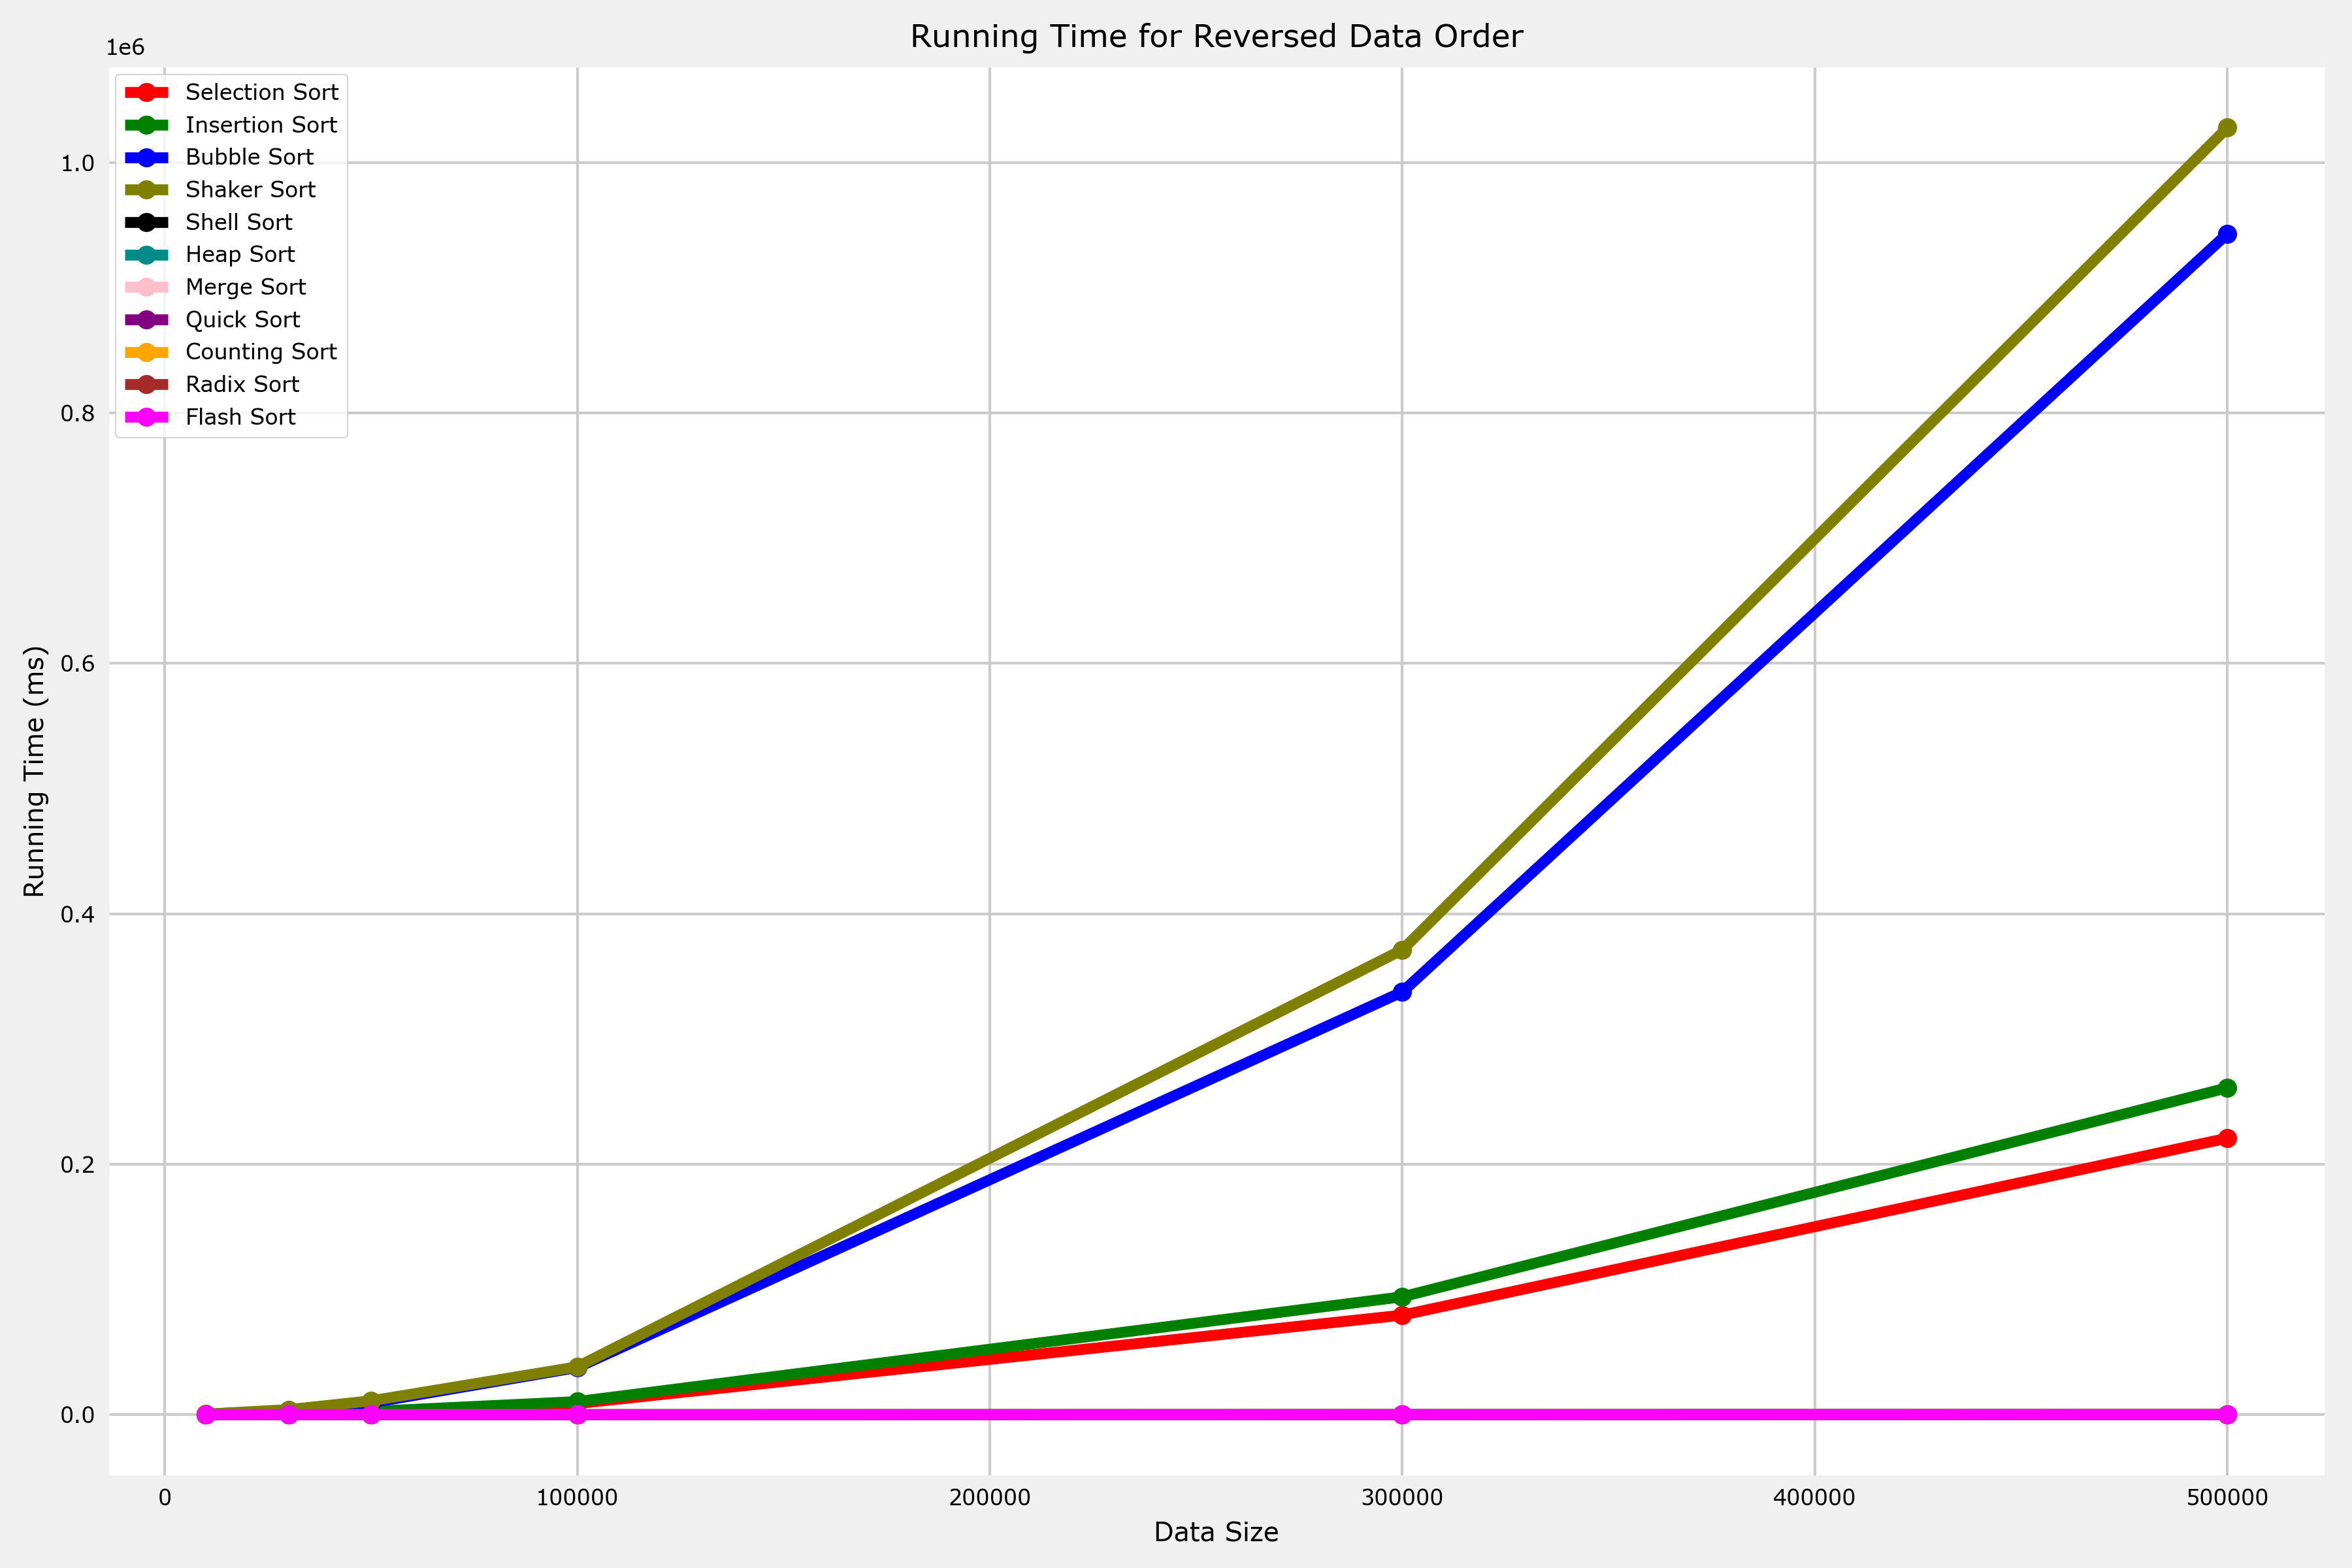
\includegraphics[width=\textwidth]{experimental_result/images/reversed_running_time.png}
    \caption{Thời gian chạy của 11 thuật toán với dữ liệu đảo ngược}
    \label{fig:reversed_running_time}
\end{figure}

\textbf{3.2.1.4. Dữ liệu đảo ngược}


Đối với bộ dữ liệu đảo ngược, Shaker Sort có thời gian chạy tương đối bằng Bubble Sort. Thời gian thực thi của Selection Sort và Insertion Sort khá giống nhau. Shaker Sort và Bubble Sort thể hiện khuynh hướng tăng mạnh hơn so với Selection Sort và Insertion Sort khi gặp kích thước dữ liệu lớn. Hình \ref{fig:reversed_running_time_filtered} có được sau khi bỏ qua 4 thuật toán nhóm cơ bản.

\begin{figure}[H]
    \centering
    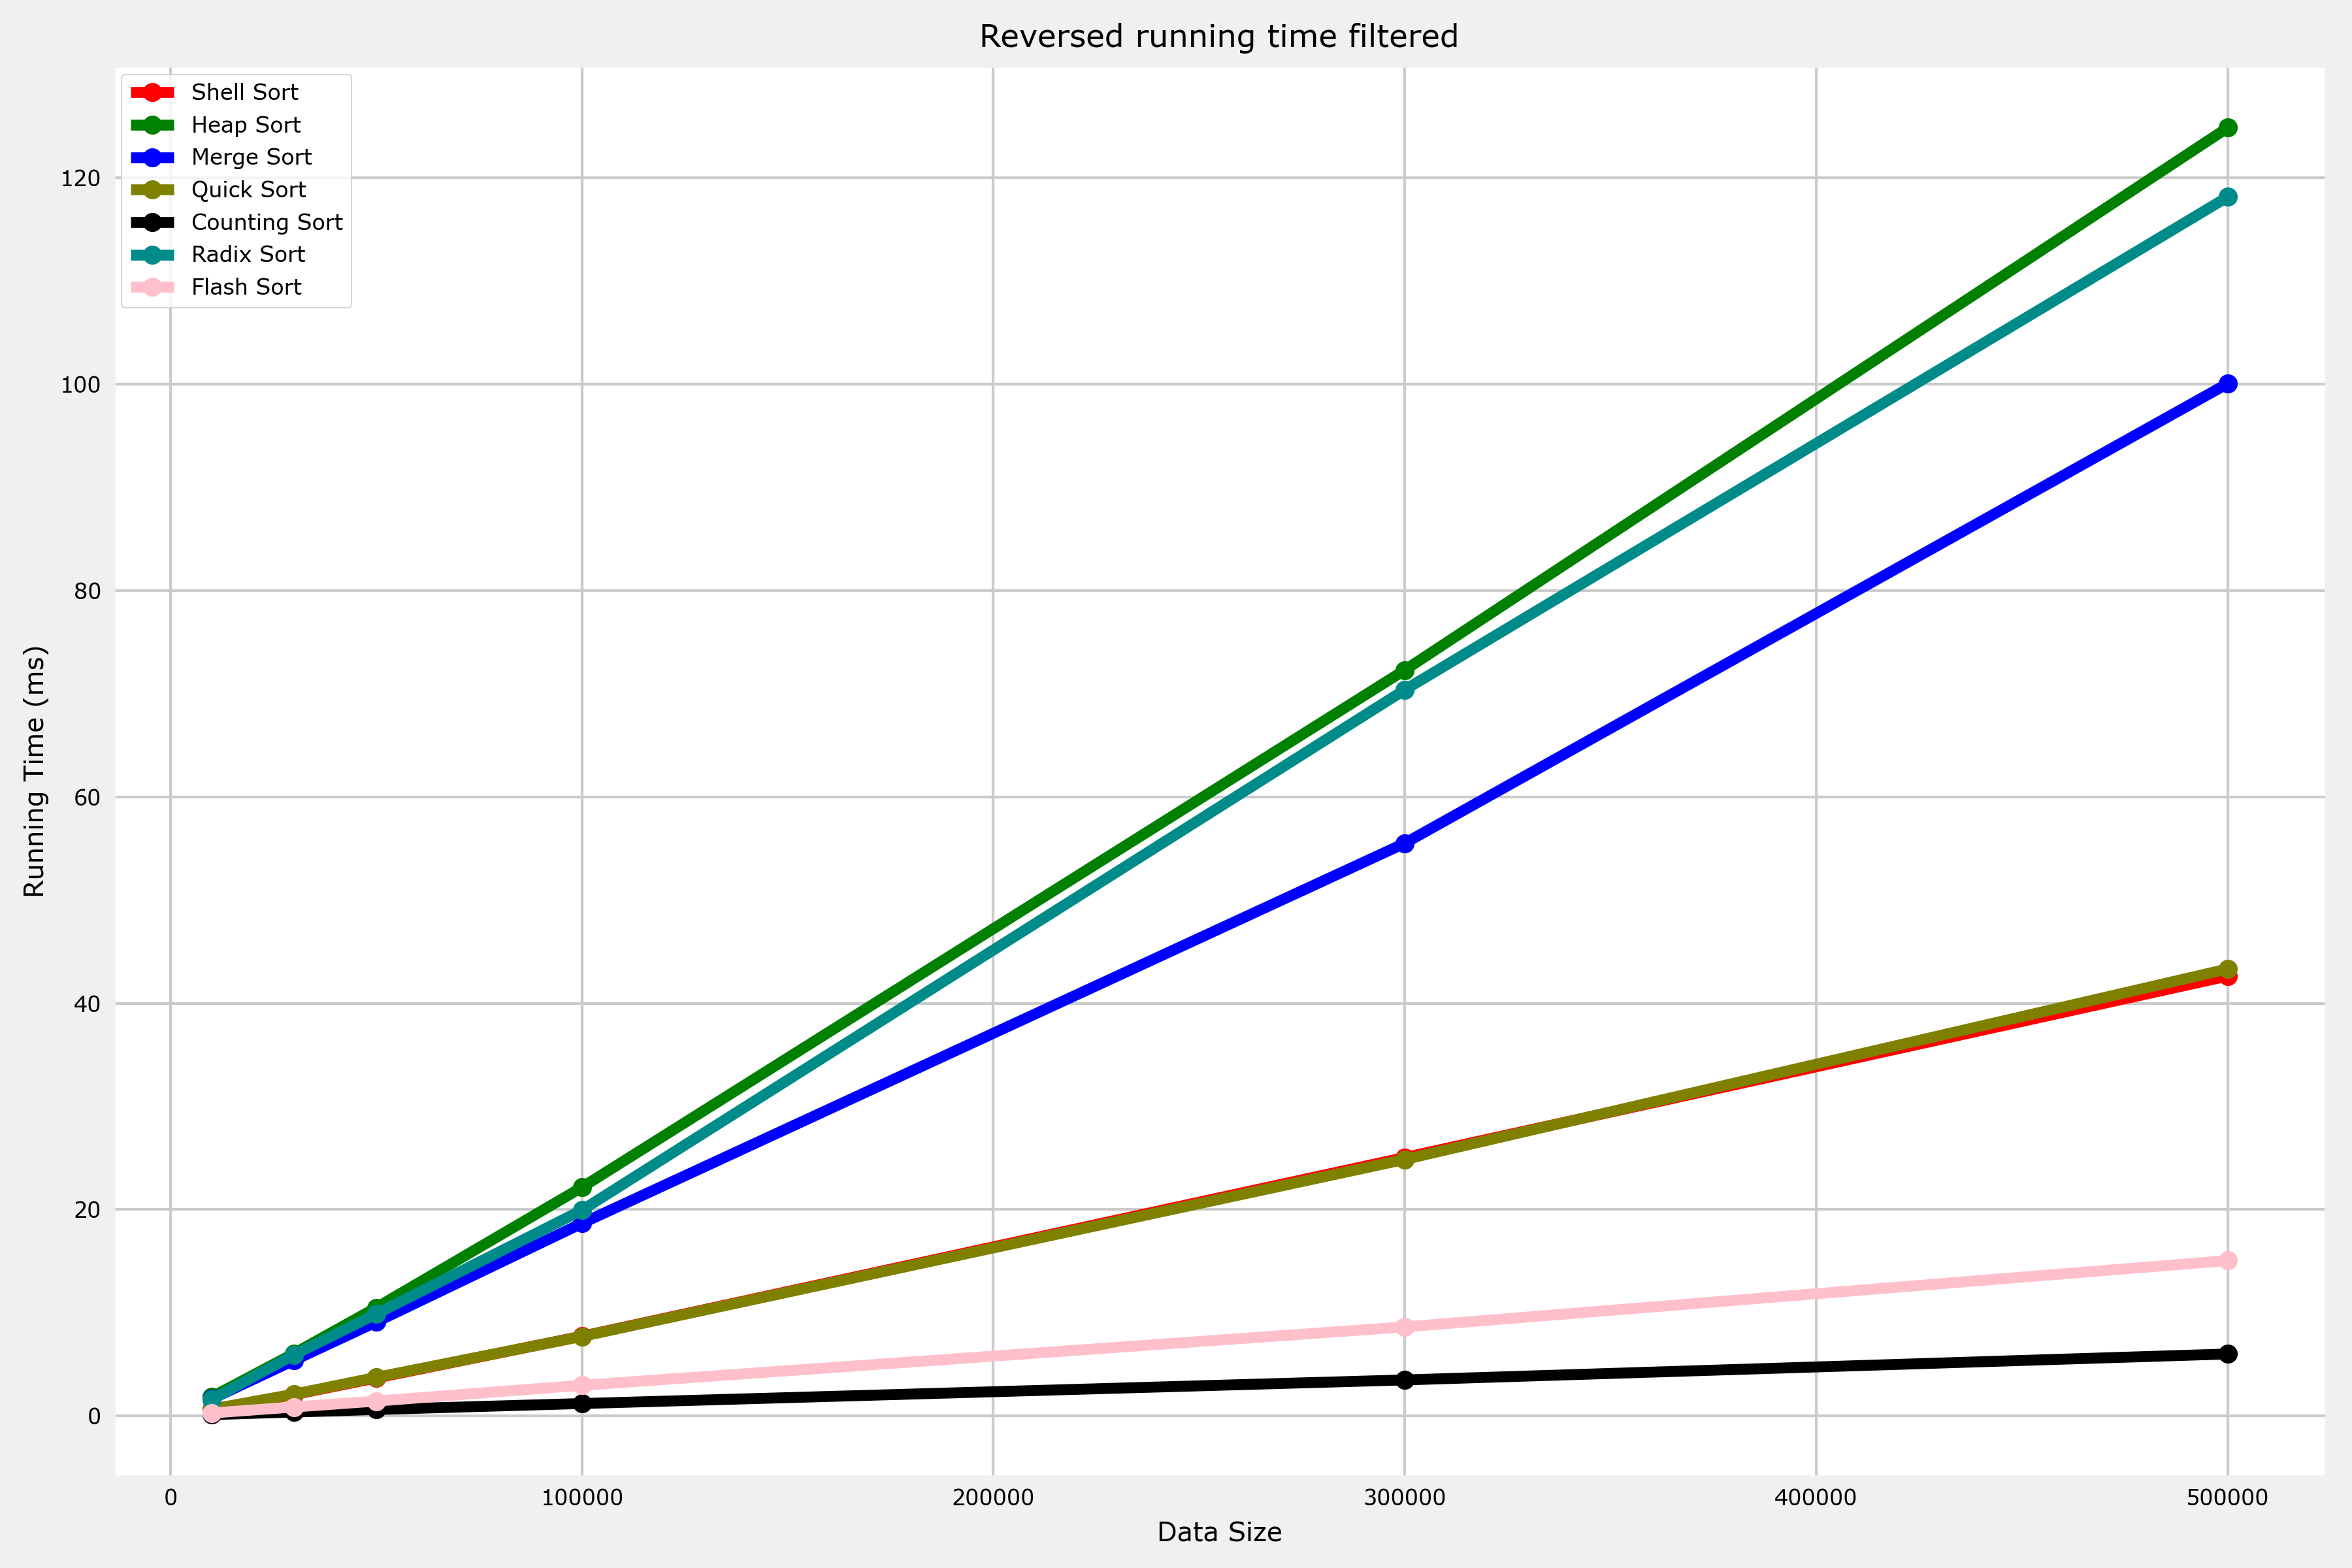
\includegraphics[width=\textwidth]{experimental_result/images/reversed_running_time_filtered.png}
    \caption{Thời gian chạy của 11 thuật toán với dữ liệu đảo ngược sau khi loại bỏ outlier}
    \label{fig:reversed_running_time_filtered}
\end{figure}


Ba thuật toán Heap Sort, Radix Sort, Merge Sort đã thể hiện được tính ổn đỉnh trong cả tất cả trường hợp. Hai thuật toán nhanh nhất vẫn là Counting Sort và Flash Sort. Đường biểu diễn của Quick Sort và Shell Sort khá trùng nhau.








\subsubsection{Biểu đồ số phép so sánh}

Đầu tiên, tiến hành vẽ tất cả biểu đồ trên các thứ tự khác nhau của 11 thuật toán, được hình \ref{fig:all_the_number_of_comparisons_for_each_algorithm_of_each_data_order}.

\begin{figure}[H]
    \centering
    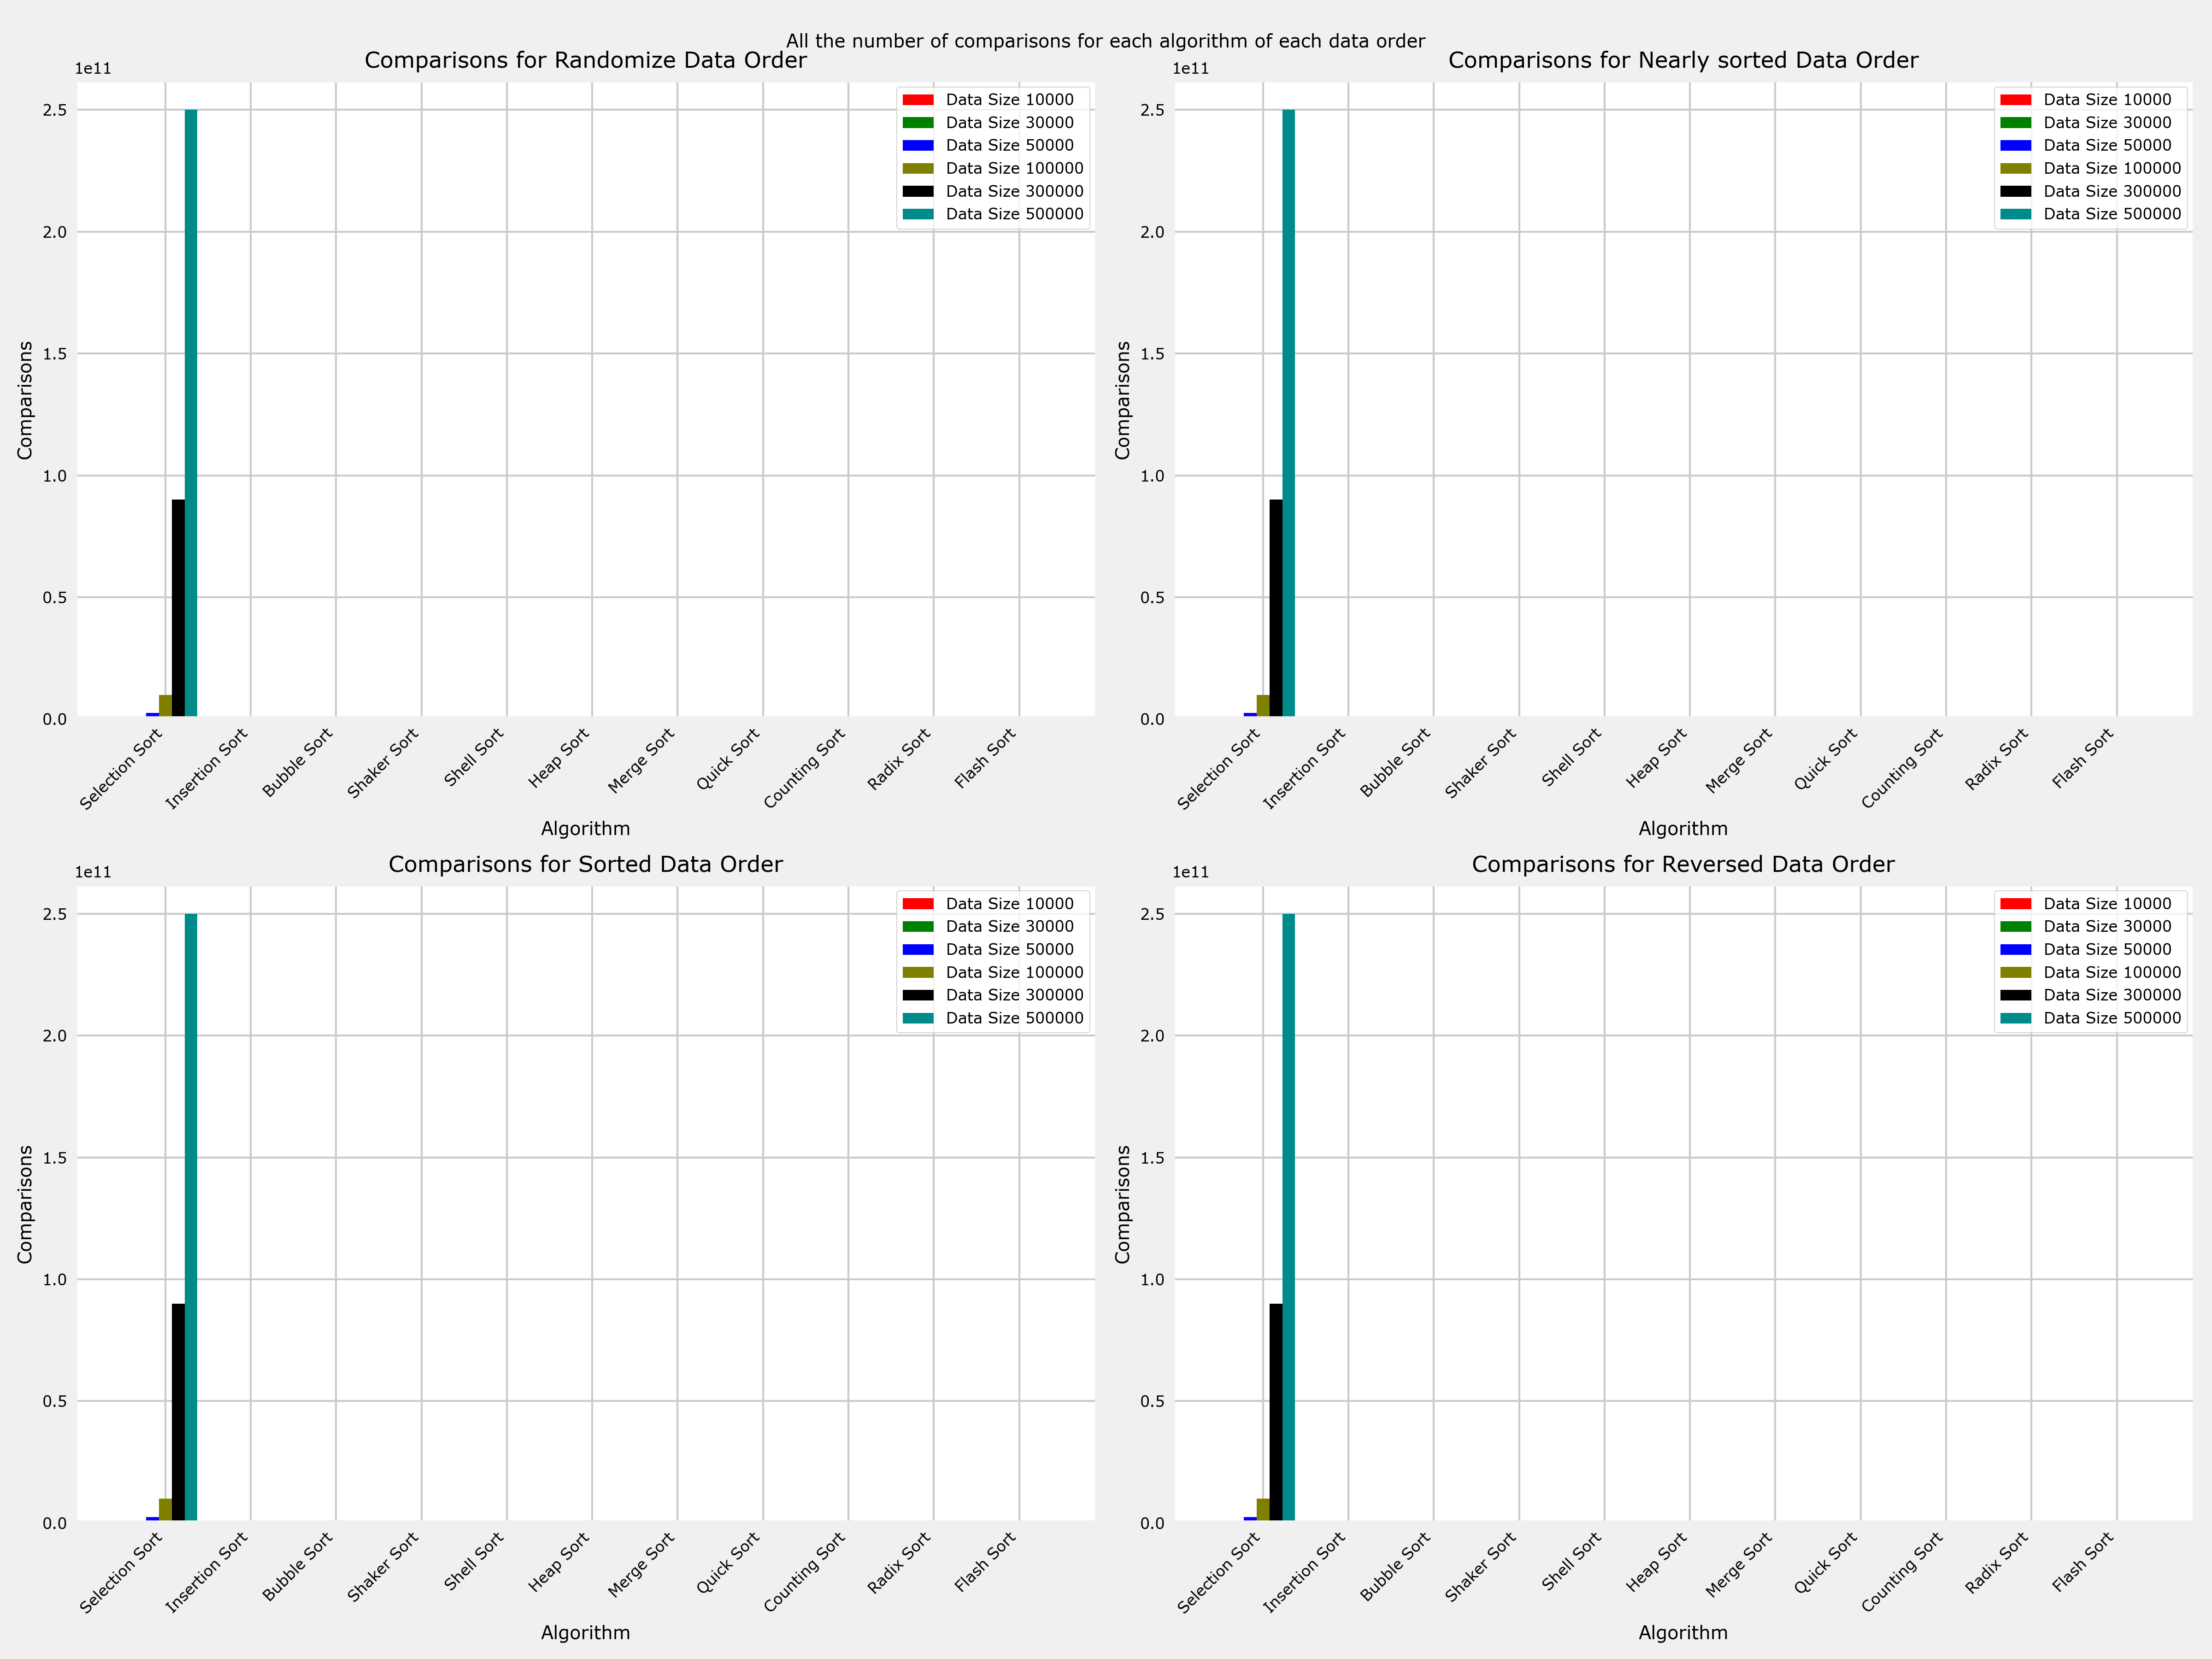
\includegraphics[width=\textwidth]{experimental_result/images/all_the_number_of_comparisons_for_each_algorithm_of_each_data_order.png}
    \caption{Số phép so sánh của 11 thuật toán với tất cả trường hợp của dữ liệu}
    \label{fig:all_the_number_of_comparisons_for_each_algorithm_of_each_data_order}
\end{figure}

Dễ thấy, Selection Sort số lượng phép so sánh vượt trội hơn 10 thuật toán còn lại, và đạt đến 2500049999 phép so sánh. Do đó, các thuật toán còn lại không thể nhìn thấy được trên biểu đồ. Selection Sort tăng rất mạnh khi gặp kích thước dữ liệu tăng dần, thể hiện độ phức tạp thời gian trung bình $\Theta(n^2)$. Vì thuật toán này luôn duyệt tất cả trường hợp có thể xảy ra, không dừng sớm khi đã sắp xếp xong nên số lượng phép so sánh là như nhau đối với tất cả trường hợp của mảng trong thực nghiệm (Phần 3.1 \ref{subsec:experimental_result}).  

Từ đây bỏ qua Selection Sort để thuận tiện cho việc trực quan hóa dữ liệu.


\begin{figure}[H]
    \centering
    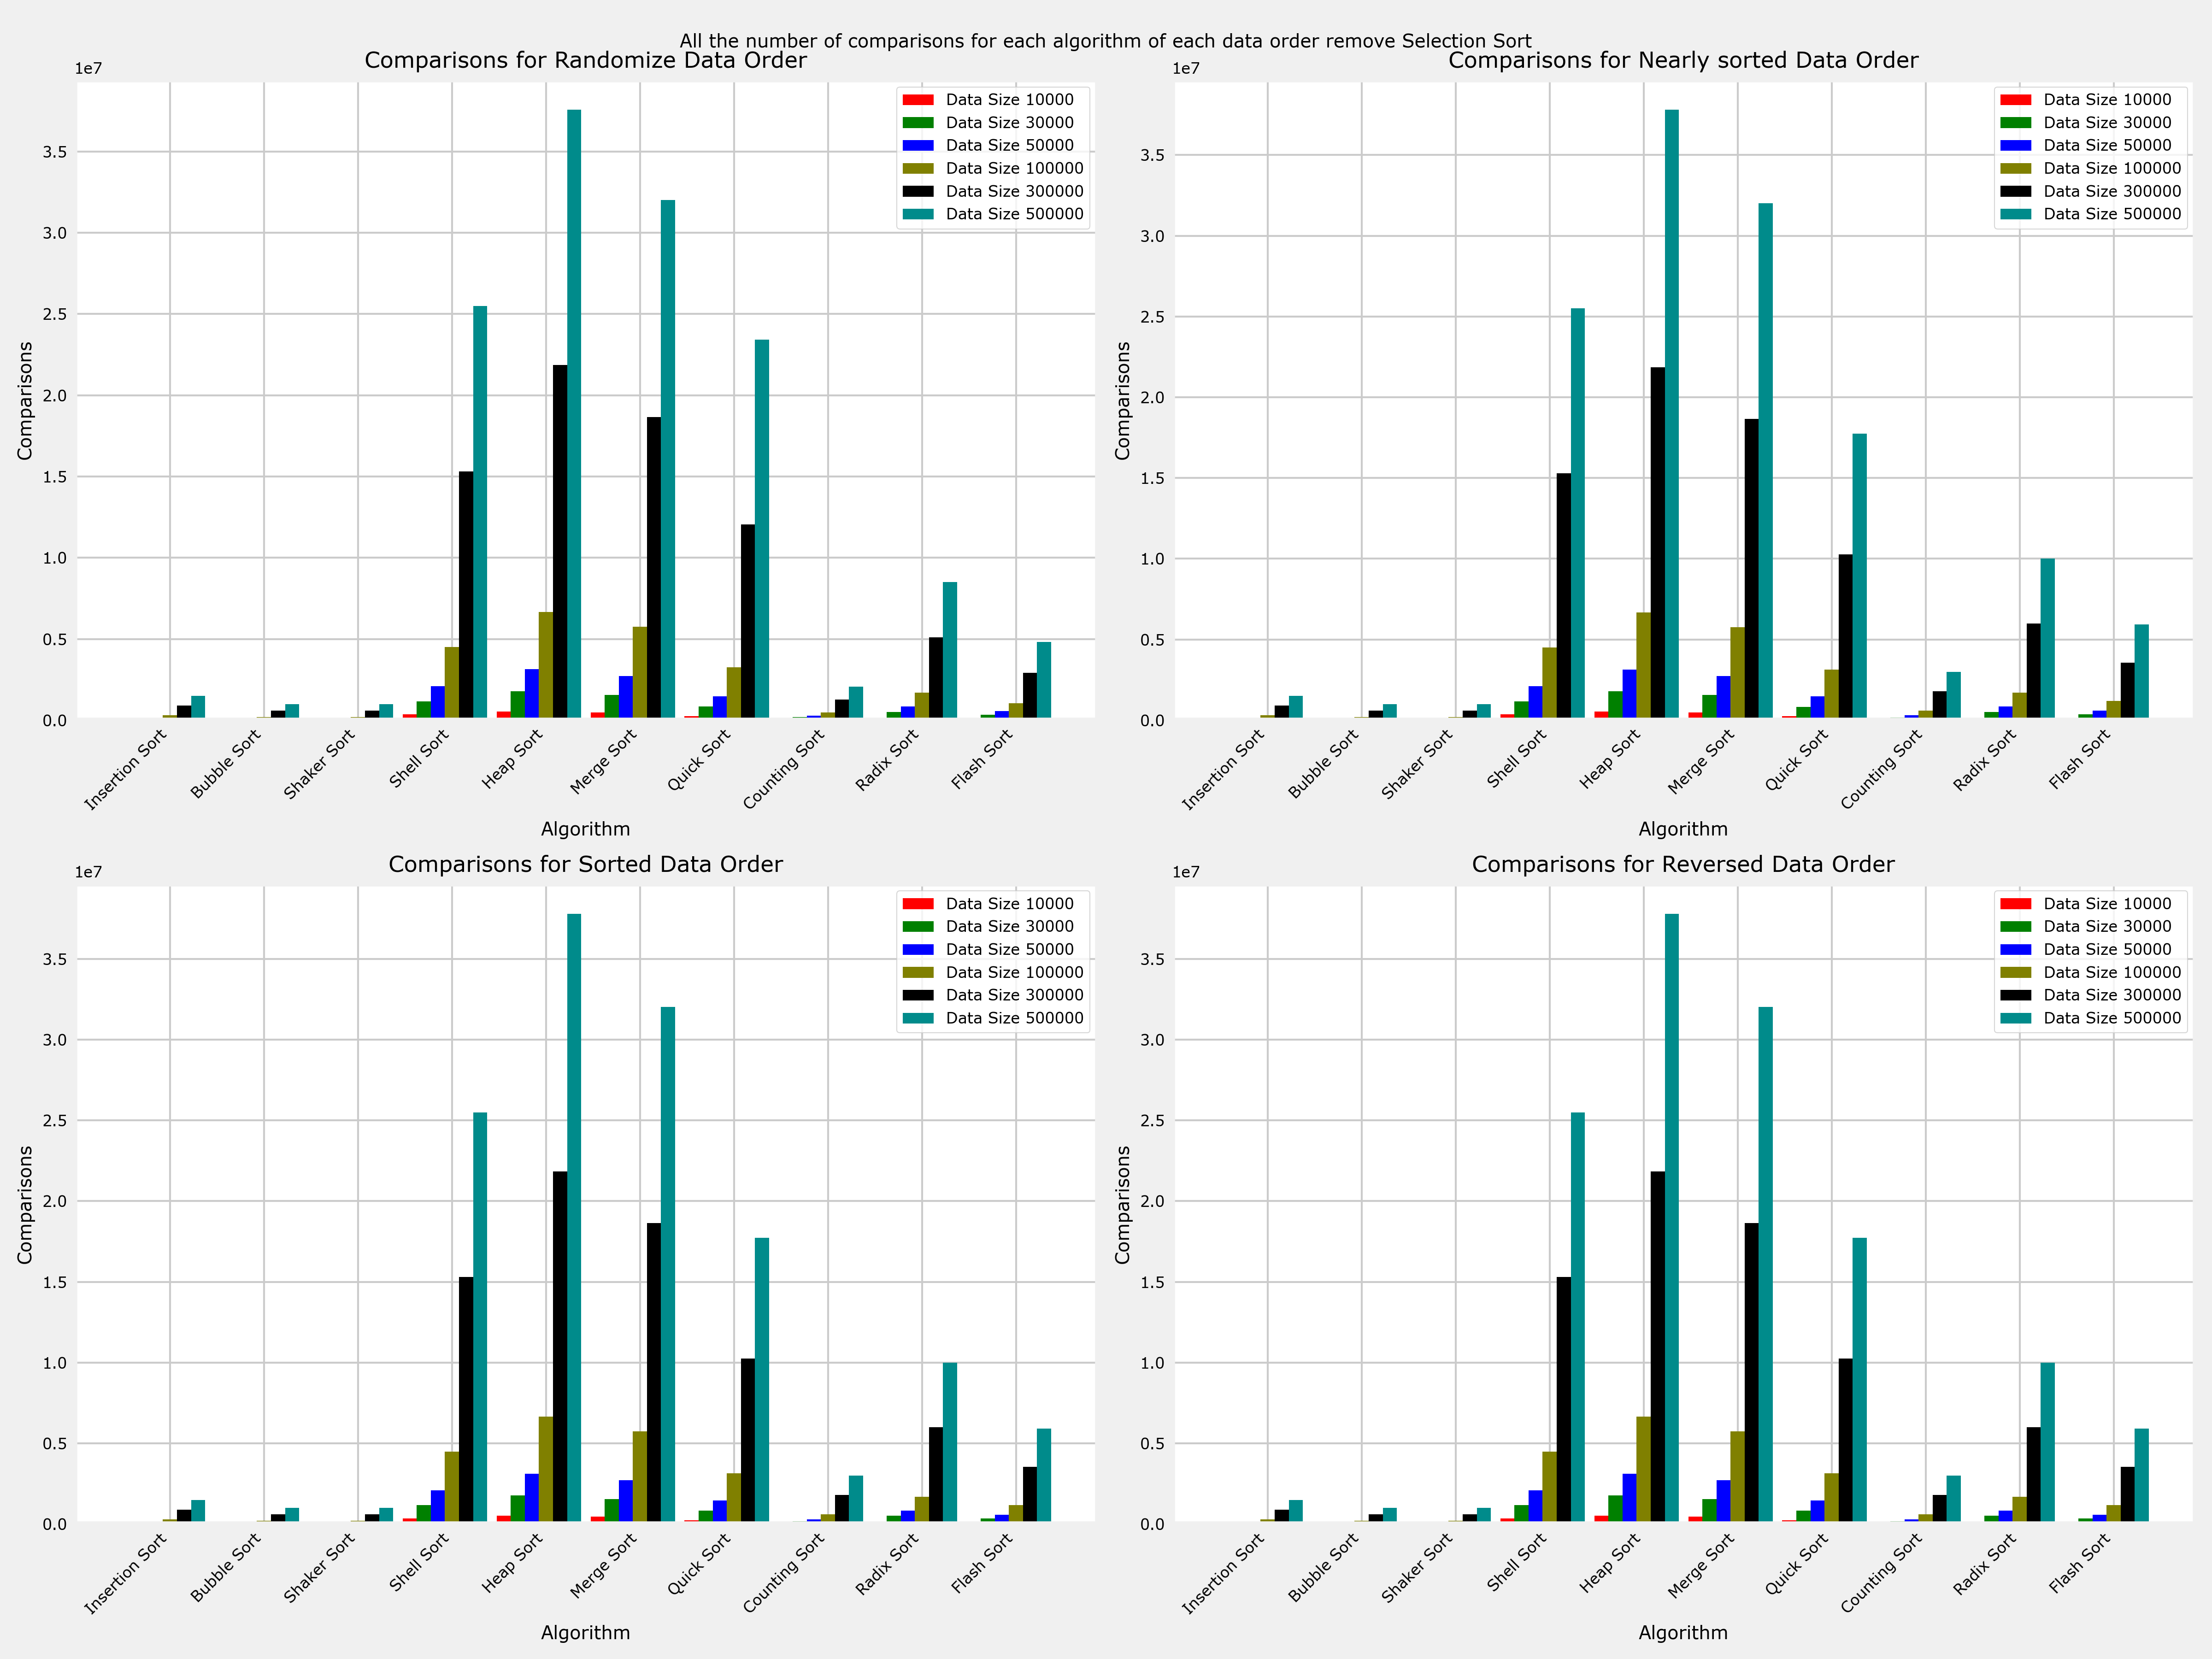
\includegraphics[width=\textwidth]{experimental_result/images/all_the_number_of_comparisons_for_each_algorithm_of_each_data_order_remove_selection_sort.png}
    \caption{Số phép so sánh của 10 thuật toán với tất cả trường hợp của dữ liệu (không có Selection Sort)}
    \label{fig:all_the_number_of_comparisons_for_each_algorithm_of_each_data_order_remove_selection_sort}
\end{figure}


Từ biểu đồ \ref{fig:all_the_number_of_comparisons_for_each_algorithm_of_each_data_order_remove_selection_sort} chia các thuật toán thành 3 nhóm chính: 
\begin{itemize}
    \item Nhóm 1: Insertion Sort, Bubble Sort, Shaker Sort 
    \item Nhóm 2: Shell Sort, Heap Sort, Merge Sort, Quick Sort
    \item Nhóm 3: Counting Sort, Radix Sort, Flash Sort
\end{itemize}

Nhóm 1 có số lượng phép so sánh ít nhất trong tất cả trường hợp của dữ liệu. Ngược lại, nhóm 2 lại có số phép sánh nhiều nhất trong ba nhóm.

Tiến hành nhìn kĩ hơn vào từng nhóm thuật toán.

\textbf{Nhóm 1}

\begin{figure}[H]
    \centering
    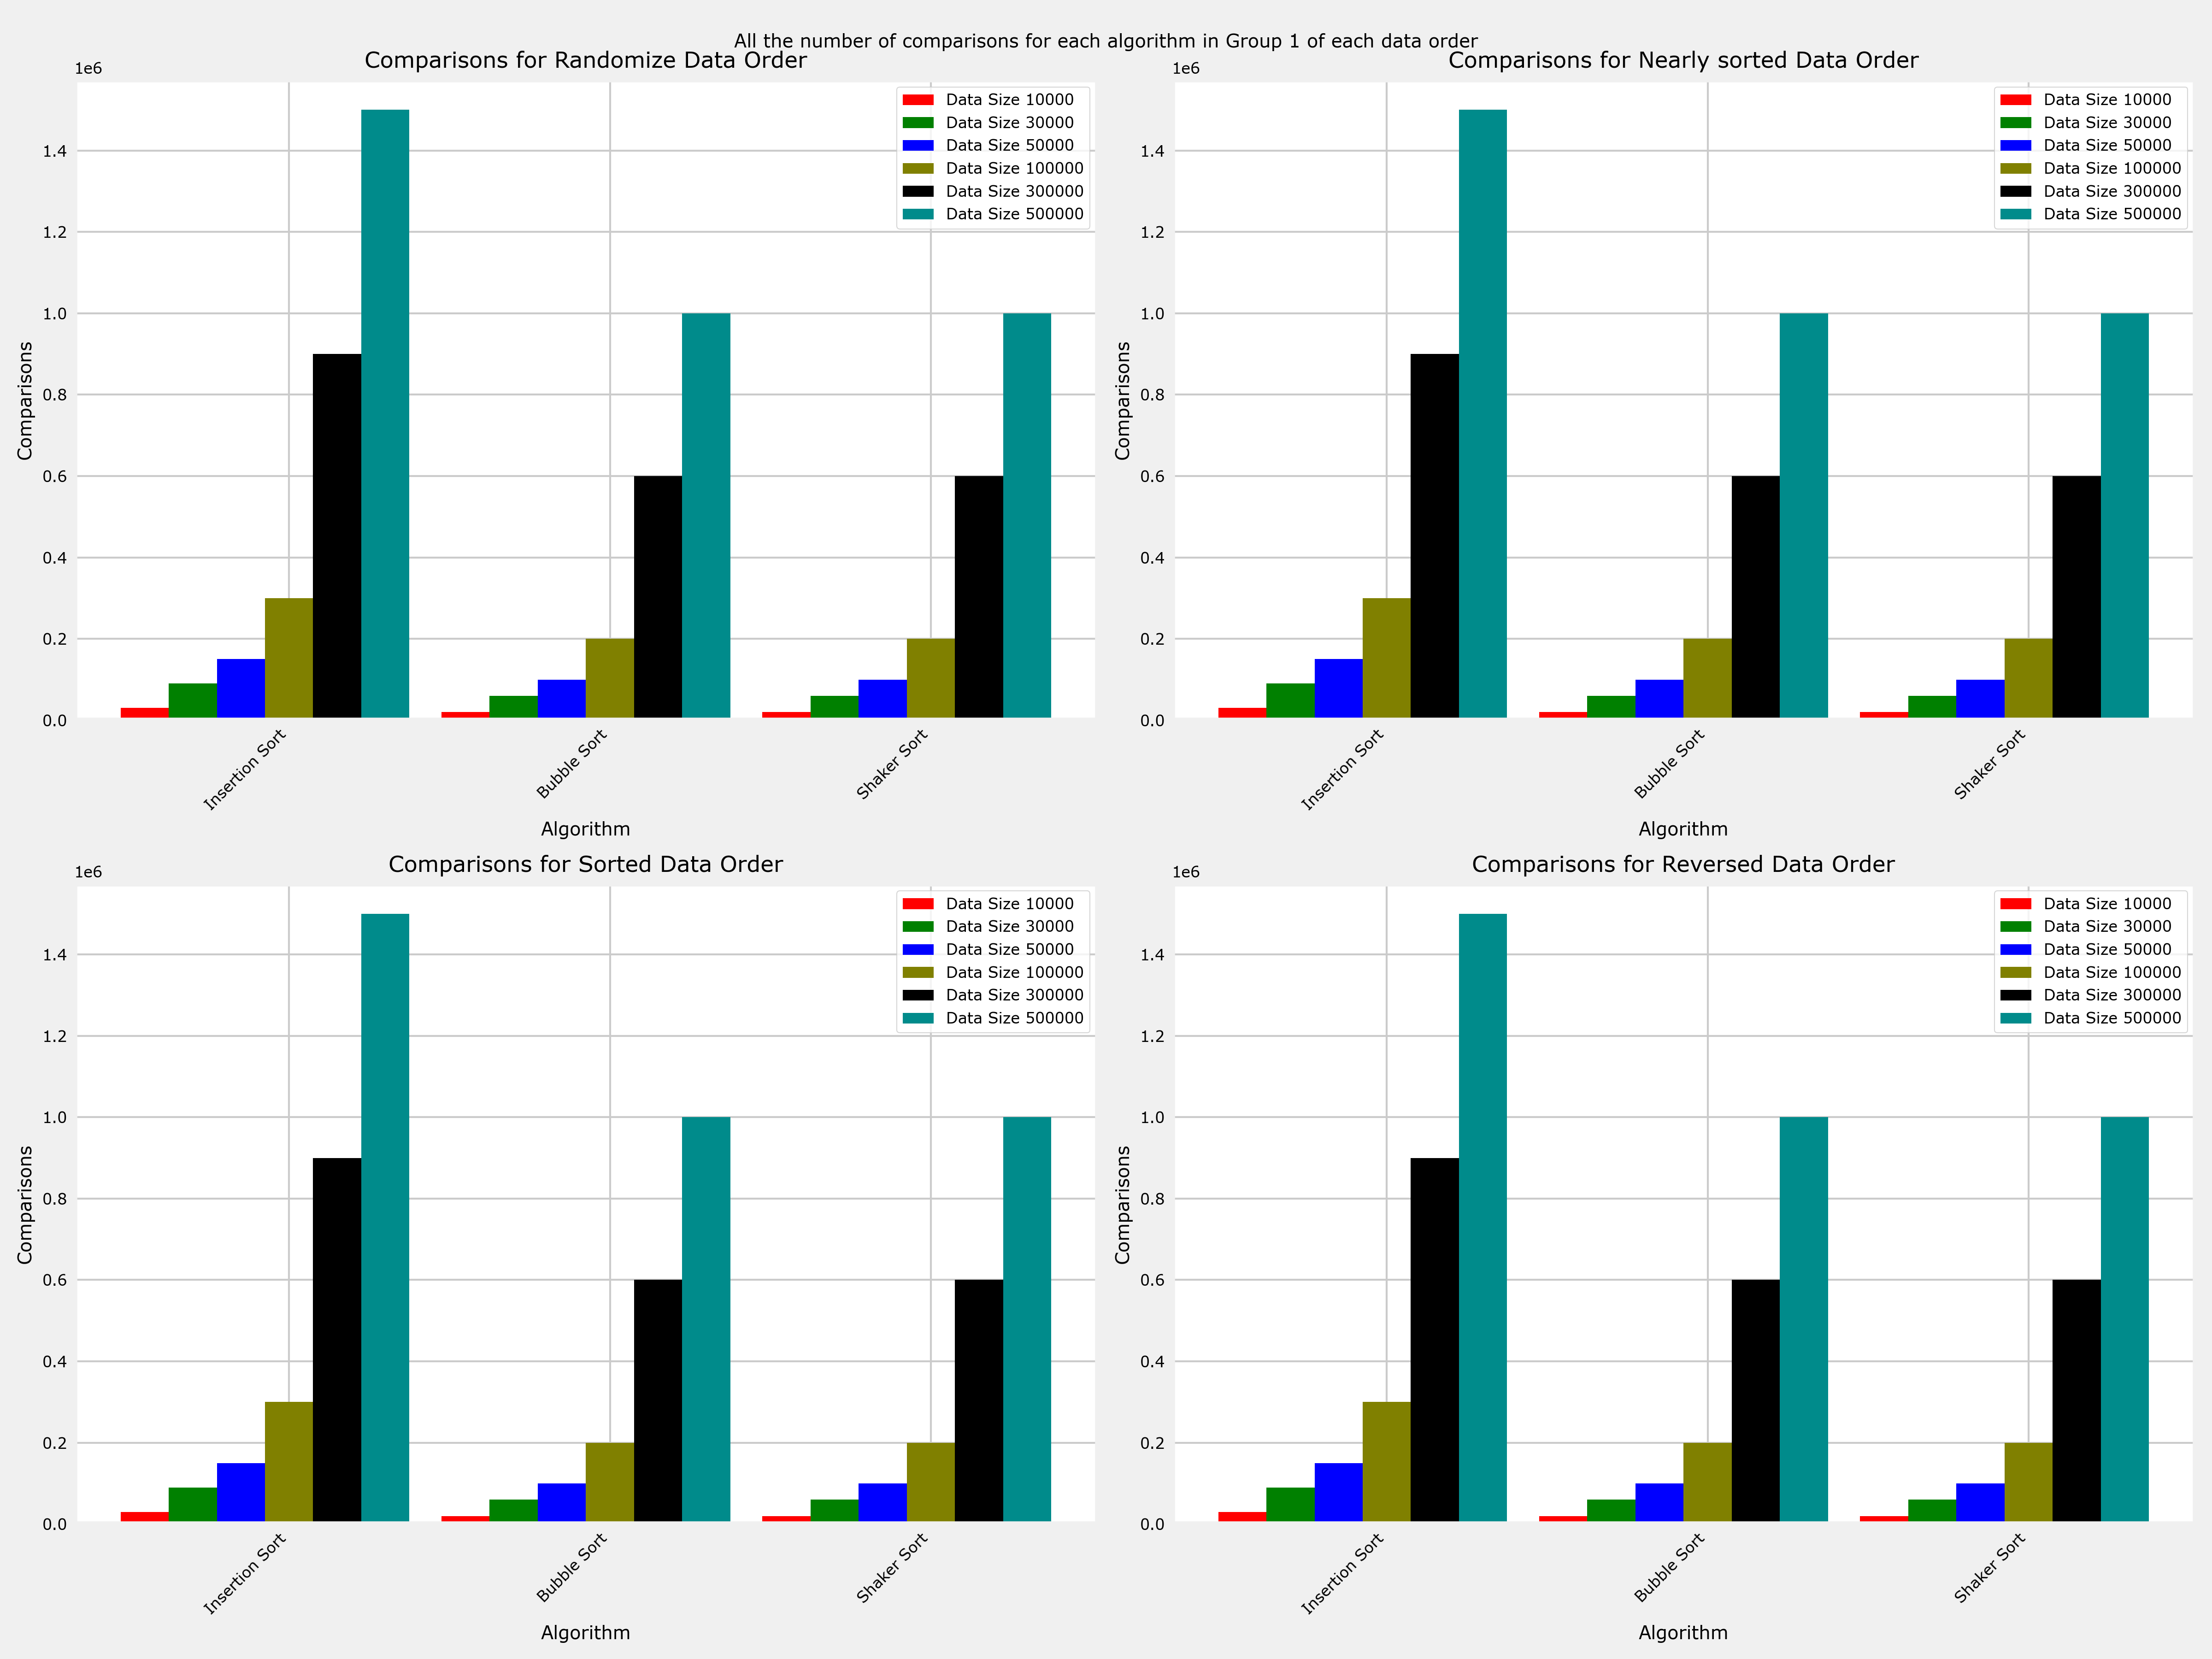
\includegraphics[width=\textwidth]{experimental_result/images/all_the_number_of_comparisons_for_each_algorithm_in_group_1_of_each_data_order.png}
    \caption{Số phép so sánh của Insertion Sort, Bubble Sort, Shaker Sort với tất cả trường hợp của dữ liệu}
    \label{fig:all_the_number_of_comparisons_for_each_algorithm_in_group_1_of_each_data_order}
\end{figure}

Ngoại trừ, Insertion Sort có độ phức tạp thời gian $\Theta(n)$ trong trường hợp mảng đã sắp xếp, các thuật toán nhóm này đều có xu hướng tăng theo hàm đa thức bậc hai. Điều này do các thuật toán này đều có độ phức tạp thời gian là hàm đa thức bậc hai cho trong hầu hết các trường hợp. 


\textbf{Nhóm 2}

\begin{figure}[H]
    \centering
    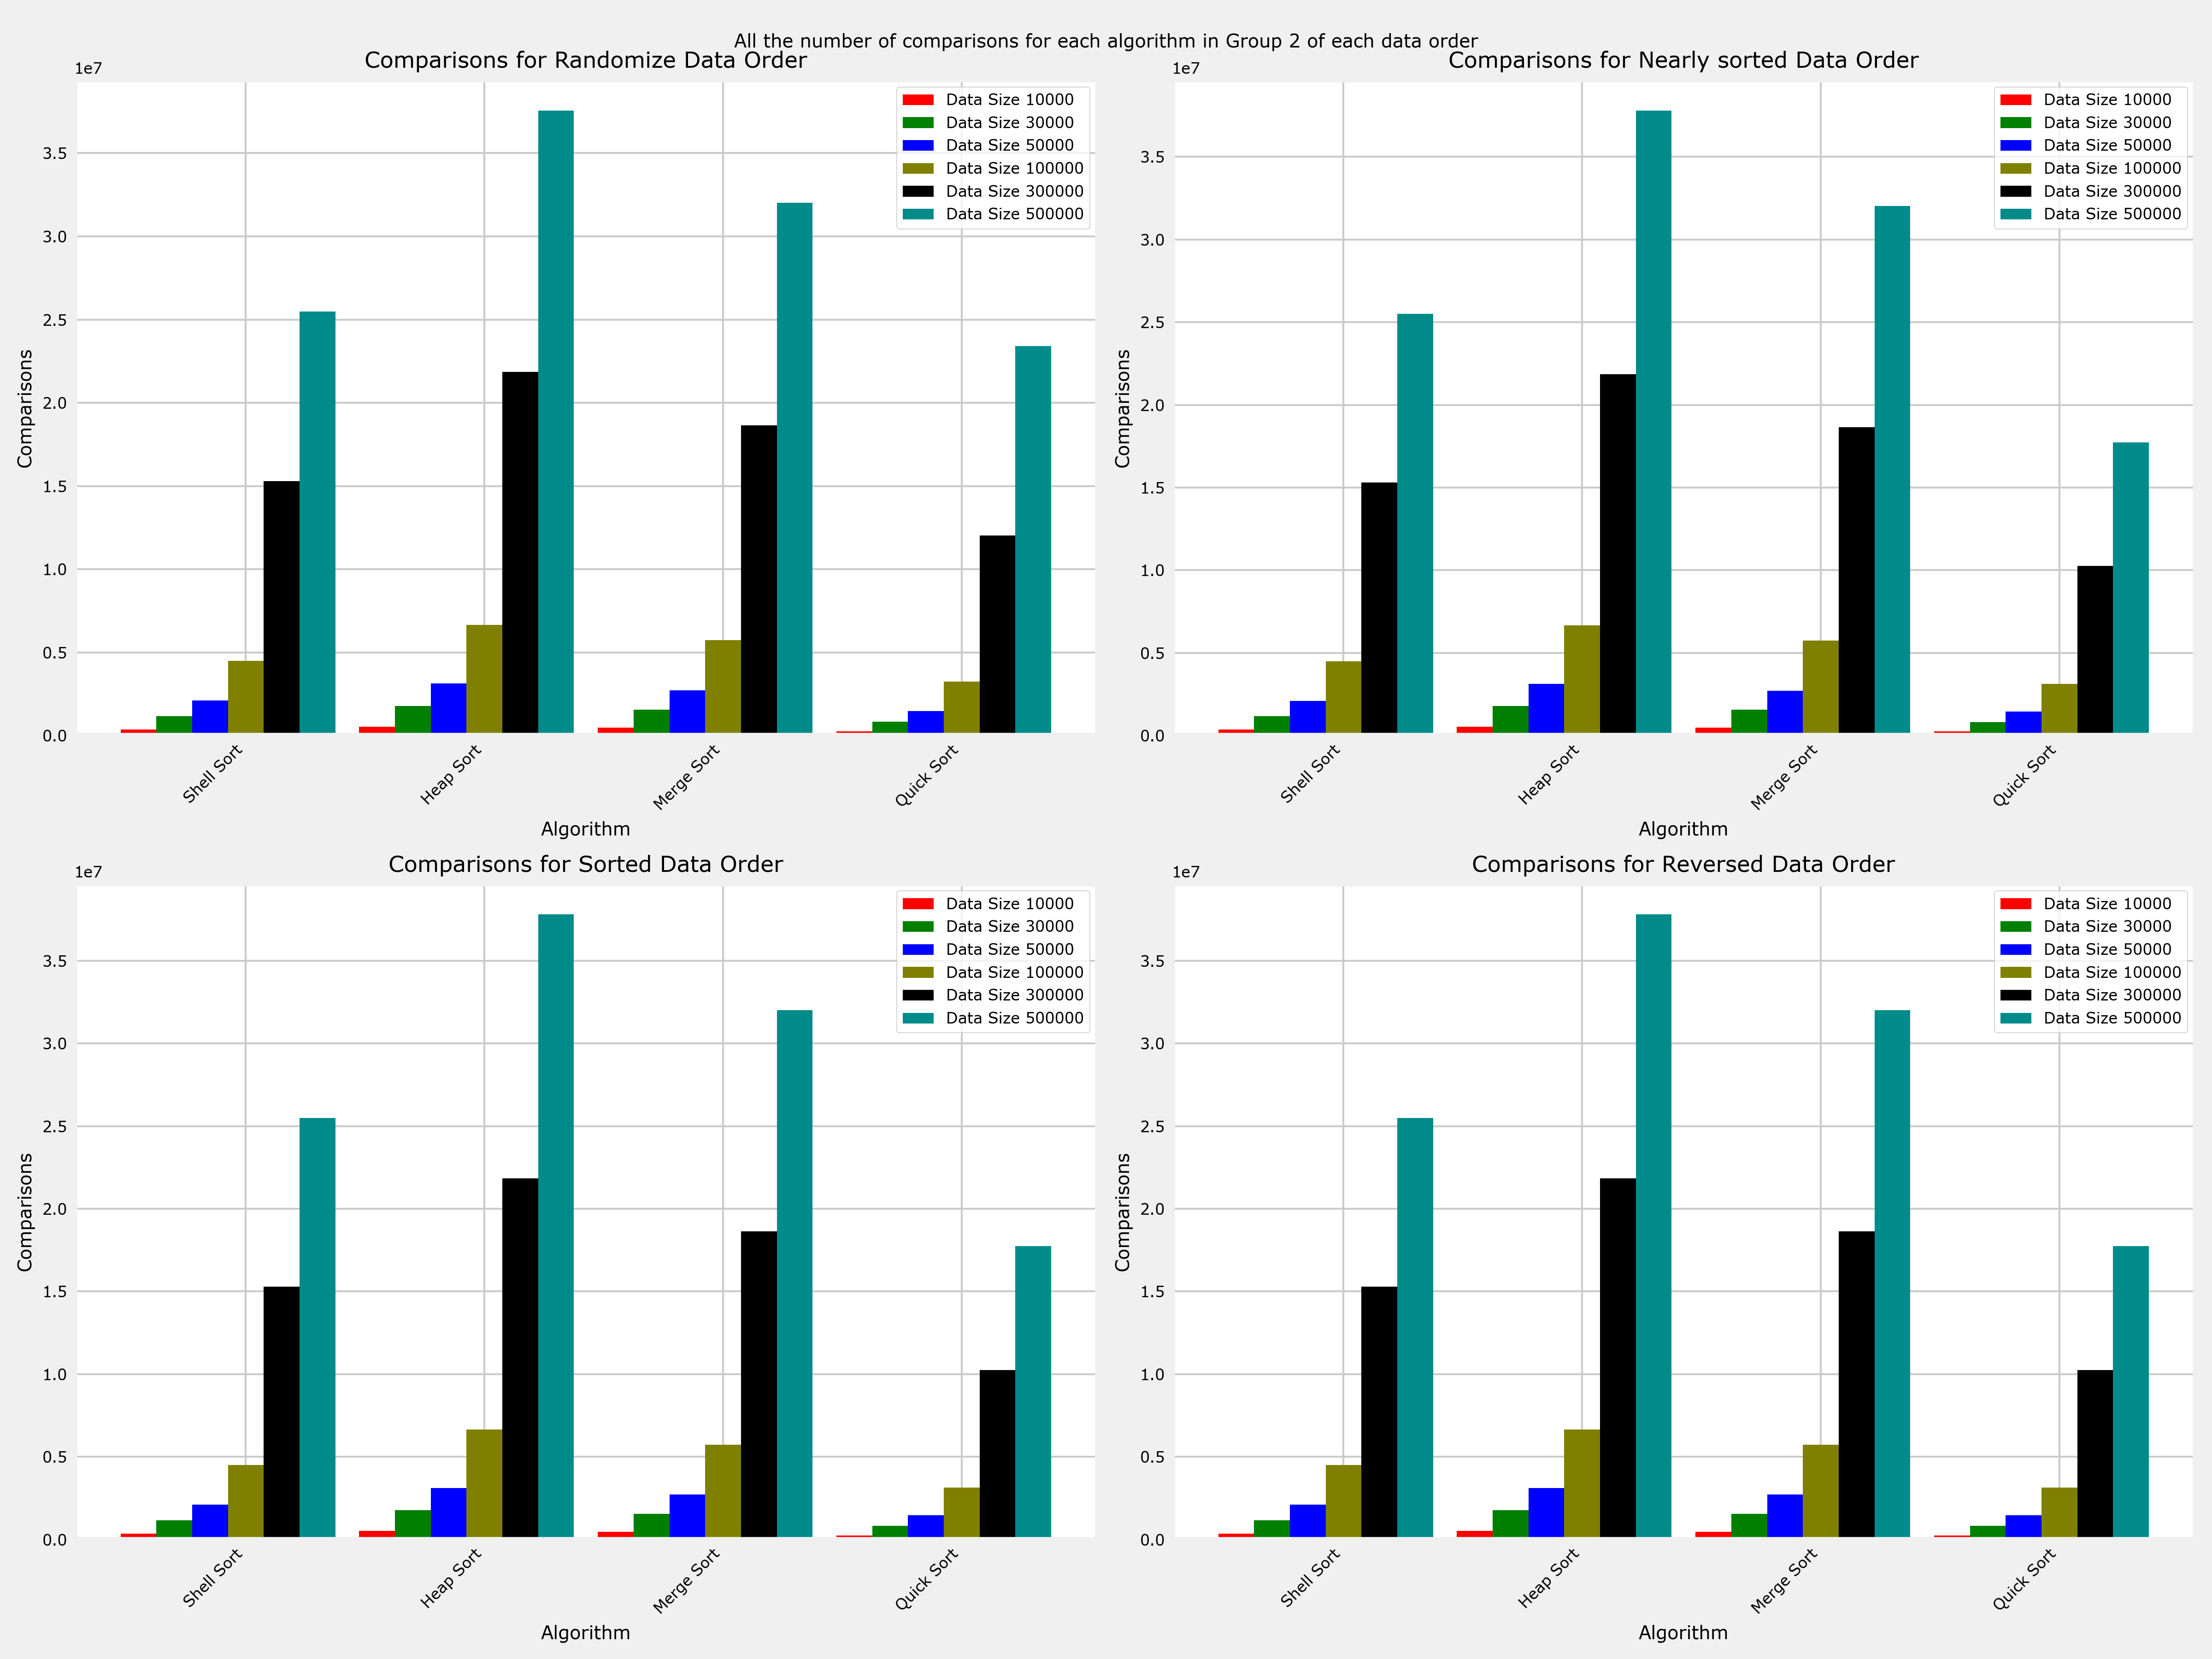
\includegraphics[width=\textwidth]{experimental_result/images/all_the_number_of_comparisons_for_each_algorithm_in_group_2_of_each_data_order.png}
    \caption{Số phép so sánh của Shell Sort, Heap Sort, Merge Sort, Quick Sort với tất cả trường hợp của dữ liệu}
    \label{fig:all_the_number_of_comparisons_for_each_algorithm_in_group_2_of_each_data_order}
\end{figure}

Đến với nhóm 2, số lượng phép so sánh của các thuật toán này không có hầu như không có sự thay đổi khi đi qua tất cả trường hợp của dữ liệu. Heap Sort có số lượng phép so sánh lớn nhất trong nhóm này, và thấp nhất là Quick Sort. 



\textbf{Nhóm 3}

\begin{figure}[H]
    \centering
    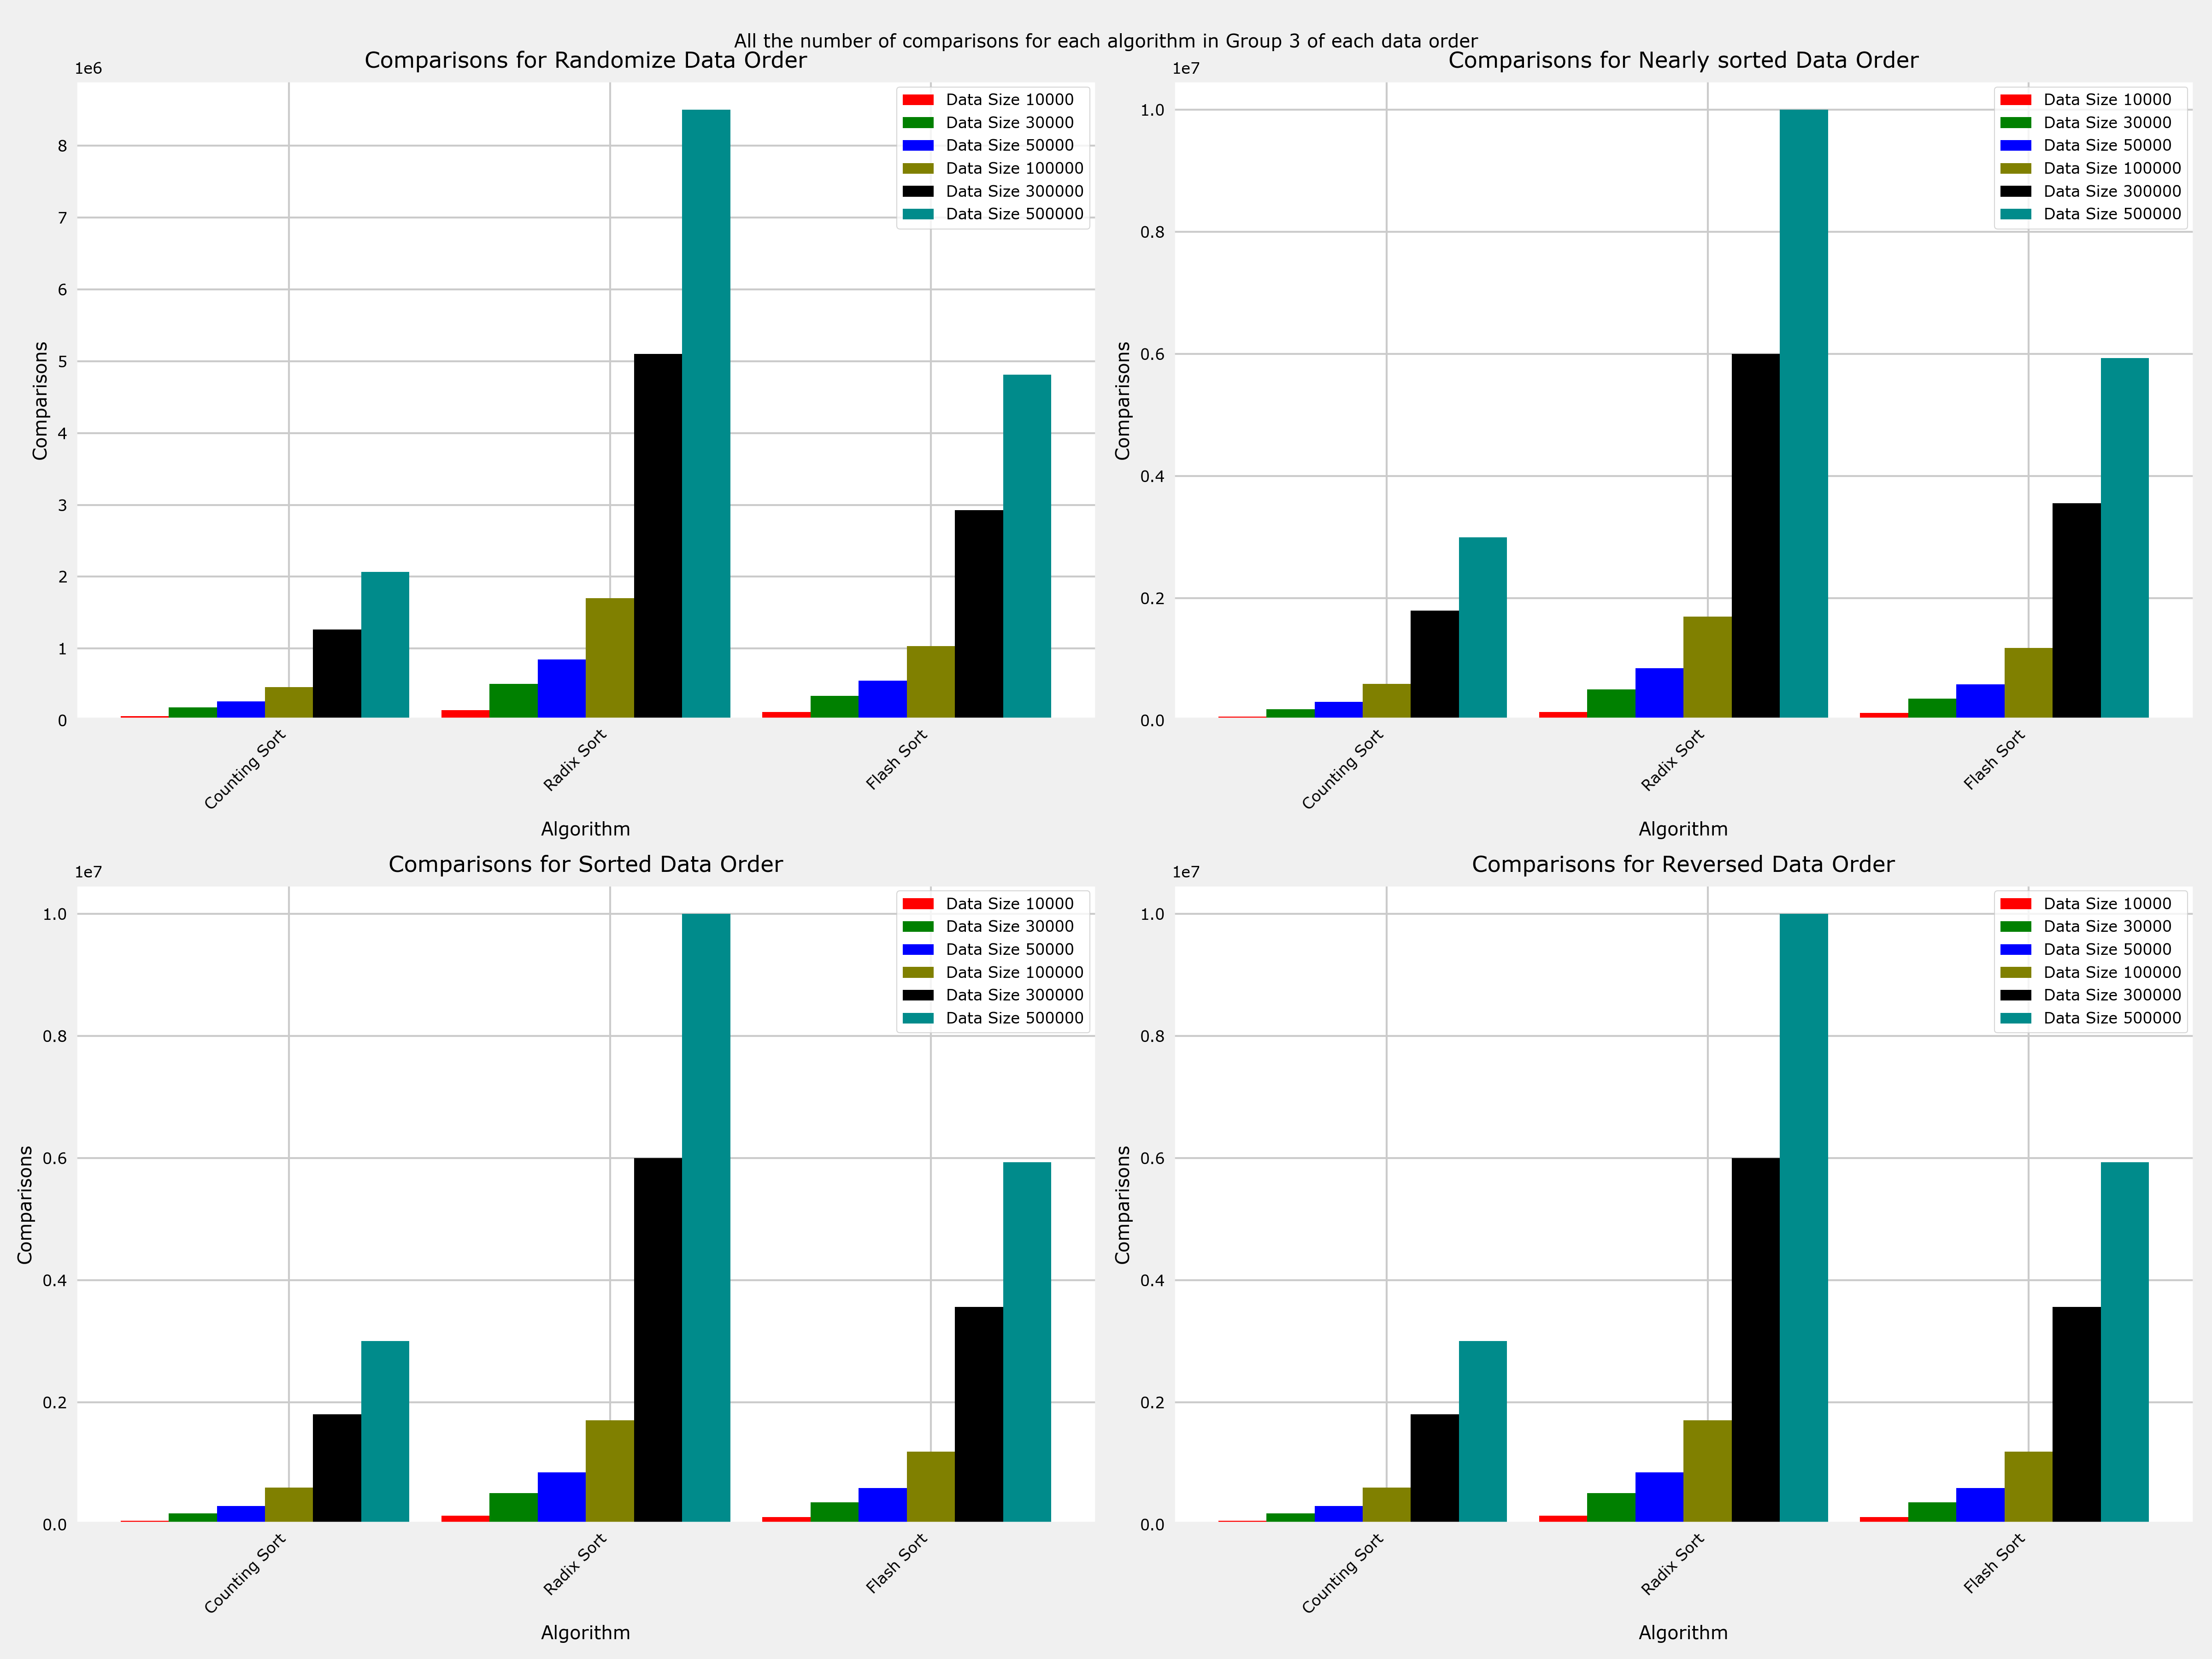
\includegraphics[width=\textwidth]{experimental_result/images/all_the_number_of_comparisons_for_each_algorithm_in_group_3_of_each_data_order.png}
    \caption{Số phép so sánh của Counting Sort, Radix Sort, Flash Sort với tất cả trường hợp của dữ liệu}
    \label{fig:all_the_number_of_comparisons_for_each_algorithm_in_group_3_of_each_data_order}
\end{figure}

Counting Sort thể hiển sự vượt trội của mình trong tất cả trường hợp, có độ tăng của số lượng phép so sánh khá thấp. Radix Sort có số phép so sánh nhiều nhất trong nhóm này. Flash Sort có số phép so sánh khá ổn định, có thể do sử dụng hàm \textbf{srand} để tạo ra dữ liệu chưa thật sự ngẫu nhiên.


\textbf{Nhận xét chung}

Các biểu đồ và hình ảnh trong phần kết quả thực nghiệm cho thấy sự khác biệt rõ rệt về hiệu suất của các thuật toán sắp xếp khi áp dụng trên các bộ dữ liệu khác nhau. 

1. **Dữ liệu ngẫu nhiên**: Các thuật toán cơ bản như Bubble Sort và Shaker Sort có thời gian chạy lớn hơn rất nhiều so với các thuật toán khác, thể hiện rõ độ phức tạp $O(n^2)$. Trong khi đó, các thuật toán như Counting Sort và Flash Sort có thời gian chạy rất nhỏ và ổn định.

2. **Dữ liệu gần sắp xếp hoàn chỉnh**: Insertion Sort có thời gian thực thi nhanh nhất, phù hợp với trường hợp tốt nhất của nó. Các thuật toán cải tiến và không so sánh như Heap Sort, Radix Sort, Merge Sort vẫn giữ được tính ổn định.

3. **Dữ liệu được sắp xếp**: Shaker Sort và Insertion Sort là hai thuật toán nhanh nhất, phù hợp với độ phức tạp thời gian $\Theta(n)$ trong trường hợp tốt nhất. Các thuật toán khác như Heap Sort, Radix Sort, Merge Sort vẫn giữ được tính ổn định.

4. **Dữ liệu đảo ngược**: Shaker Sort có thời gian chạy chậm hơn Bubble Sort, trong khi Selection Sort và Insertion Sort có thời gian thực thi tương đối giống nhau. Các thuật toán như Heap Sort, Radix Sort, Merge Sort vẫn thể hiện được tính ổn định.

5. **Số phép so sánh**: Selection Sort có số lượng phép so sánh vượt trội, đạt đến 2500049999 phép so sánh. Các thuật toán khác được chia thành ba nhóm chính: Nhóm 1 (Insertion Sort, Bubble Sort, Shaker Sort) có số lượng phép so sánh ít nhất, Nhóm 2 (Shell Sort, Heap Sort, Merge Sort, Quick Sort) có số phép so sánh nhiều nhất, và Nhóm 3 (Counting Sort, Radix Sort, Flash Sort) có số phép so sánh ổn định và thấp nhất.

Nhìn chung, các thuật toán cải tiến và không so sánh như Counting Sort, Flash Sort, Heap Sort, Radix Sort, Merge Sort thể hiện hiệu suất tốt và ổn định hơn so với các thuật toán cơ bản như Bubble Sort, Shaker Sort, và Selection Sort.
\section{Tổ chức mã nguồn}

Các thuật toán tiến hành trong bài báo cáo này được tổ chức thành các thư mục
\begin{itemize}
    \item \textbf{sorting-algorithm}: Gồm các file chứa các hàm cho từng thuật toán. Mỗi thuật toán sẽ có 2 phiên bản: một phiên bản gốc dùng để thực hiện sắp xếp và đo thời gian chạy, một phiên bản có thêm tham chiếu của biến đếm để tiến hành đếm các phép so sánh. 
    \item \textbf{helper}:
    \begin{itemize}
        \item \textbf{DataGenerator.hpp}: Chứa cách hàm phát sinh dữ liệu.
        \item \textbf{ReadWriteData.hpp}: Chứa hàm đọc  dữ liệu từ file và viết dữ liệu ra file.
        \item \textbf{testFunction.hpp}: Chứa các hàm dùng để đo thời gian (đơn vị millisecond), so sánh hai thuật toán, in kết quả ra màn hình, ...
    \end{itemize}
    \item \textbf{main.cpp}: Xử lí các tham số dòng lệnh cho chương trình.
    \item \textbf{run.cpp}: File này dùng để build file main.exe, sau đó dùng file này để chạy tất cả thuật toán trên tất cả trường hợp của dữ liệu. Sau mỗi trường hợp, chương trình sẽ viết kết quả ra file result.csv.
\end{itemize}

\lstset{
    language=C++,
    basicstyle=\ttfamily\small,
    keywordstyle=\color{blue},
    commentstyle=\color{green},
    stringstyle=\color{red},
    numbers=none, % Disable line numbers
    frame=single,
}

Câu lệnh dùng để build file main.exe:
\begin{lstlisting}
g++ -std=c++17 -Xlinker --stack -Xlinker 17179869184 -o main.exe main.cpp ./helper/DataGenerator.hpp ./helper/ReadWriteData.hpp ./helper/testFunction.hpp ./sorting-algorithm/selection-sort.hpp ./sorting-algorithm/insertion-sort.hpp ./sorting-algorithm/bubble-sort.hpp ./sorting-algorithm/shaker-sort.hpp ./sorting-algorithm/shell-sort.hpp ./sorting-algorithm/heap-sort.hpp ./sorting-algorithm/merge-sort.hpp ./sorting-algorithm/quick-sort.hpp ./sorting-algorithm/counting-sort.hpp ./sorting-algorithm/radix-sort.hpp ./sorting-algorithm/flash-sort.hpp
\end{lstlisting}

Câu lệnh dùng để build file run.exe, lấy kết quả cho bài báo cáo này:
\begin{lstlisting}
g++ run.cpp -std=c++17 -o run
\end{lstlisting}

\textcolor{red}{Lưu ý}: Không nên copy câu các lệnh trên vì có thể khi copy sẽ chứa các khoảng trống, dấu xuống dòng.


\section{Kết luận}

Báo cáo đã trình bày và phân tích chi tiết về các thuật toán sắp xếp khác nhau, bao gồm Bubble Sort, Insertion Sort, Selection Sort, Heap Sort, Merge Sort, Quick Sort, Counting Sort, Radix Sort, và Flash Sort. Mỗi thuật toán được mô tả với các bước thực hiện cụ thể và minh họa bằng các ví dụ trực quan.

Thực nghiệm đã được tiến hành, so sánh thời gian chạy, đếm số phép so sánh của các thuật toán trên các bộ dữ liệu khác nhau: dữ liệu ngẫu nhiên, dữ liệu gần như đã sắp xếp, dữ liệu đã sắp xếp, và dữ liệu sắp xếp ngược. Kết quả thực nghiệm được trình bày chi tiết trong các bảng và biểu đồ, cho thấy sự khác biệt về hiệu suất của từng thuật toán trong các trường hợp khác nhau.

Qua quá trình thực nghiệm, nhận thấy rằng:
\begin{itemize}
    \item Các thuật toán sắp xếp đơn giản như Bubble Sort, Insertion Sort và Selection Sort có thời gian chạy chậm hơn so với các thuật toán phức tạp hơn như Heap Sort, Merge Sort và Quick Sort.
    \item Nhóm các thuật toán cơ bản (Selection Sort, Insertion Sort, Bubble Sort, Shaker Sort) có hiệu suất không ổn định qua các trường hợp của dữ liệu. Đặc biệt, hiệu suất của Selection Sort có hiệu xuất rất kém.
    \item Flash Sort và Radix Sort cho thấy hiệu suất vượt trội trong một số trường hợp nhất định, đặc biệt là với các bộ dữ liệu lớn.
    \item Merge Sort và Quick Sort là hai thuật toán có hiệu suất ổn định và thời gian chạy tốt nhất trên hầu hết các bộ dữ liệu.
    \item Counting Sort và Radix Sort có hiệu suất tốt và ổn định nhưng hai thuật toán này chỉ sử dụng được trên kiểu dữ liệu là số nguyên.
    \item item Nhóm thuật toán cải tiến (Shell Sort, Heap Sort, Merge Sort, Quick Sort) vẫn chưa thể hiện được sự khác nhau rõ ràng qua thực nghiệm.
\end{itemize}

Báo cáo này không chỉ giúp hiểu rõ hơn về các thuật toán sắp xếp mà còn cung cấp cái nhìn tổng quan về cách lựa chọn thuật toán phù hợp cho từng loại dữ liệu cụ thể. Hy vọng rằng những kết quả và phân tích trong báo cáo này sẽ là tài liệu tham khảo hữu ích cho các bạn sinh viên và những người quan tâm đến lĩnh vực cấu trúc dữ liệu và giải thuật.


% References
\cleardoublepage
\phantomsection
\addcontentsline{toc}{section}{Tài liệu tham khảo}
% \bibliographystyle{plain}
\bibliographystyle{unsrt}
\bibliography{ref/ref.bib}

% \printbibliography


% Appendix
\appendix
% Add \cleardoublepage to move appendices to next page.
% \section{Phụ lục}

\subsection{Mô tả pipeline để tạo ra file Report.pdf}
Kết quả thực nghiệm của báo cáo này được thực hiện hoàn toàn thông qua Github Action, bằng hai repository sau:
\begin{itemize}
    \item \href{https://github.com/magnusdtd/sort-project/}{sort-project}
    \item \href{https://github.com/magnusdtd/sort-project-report/}{sort-project-report}
\end{itemize}

\begin{figure}[H]
    \centering
    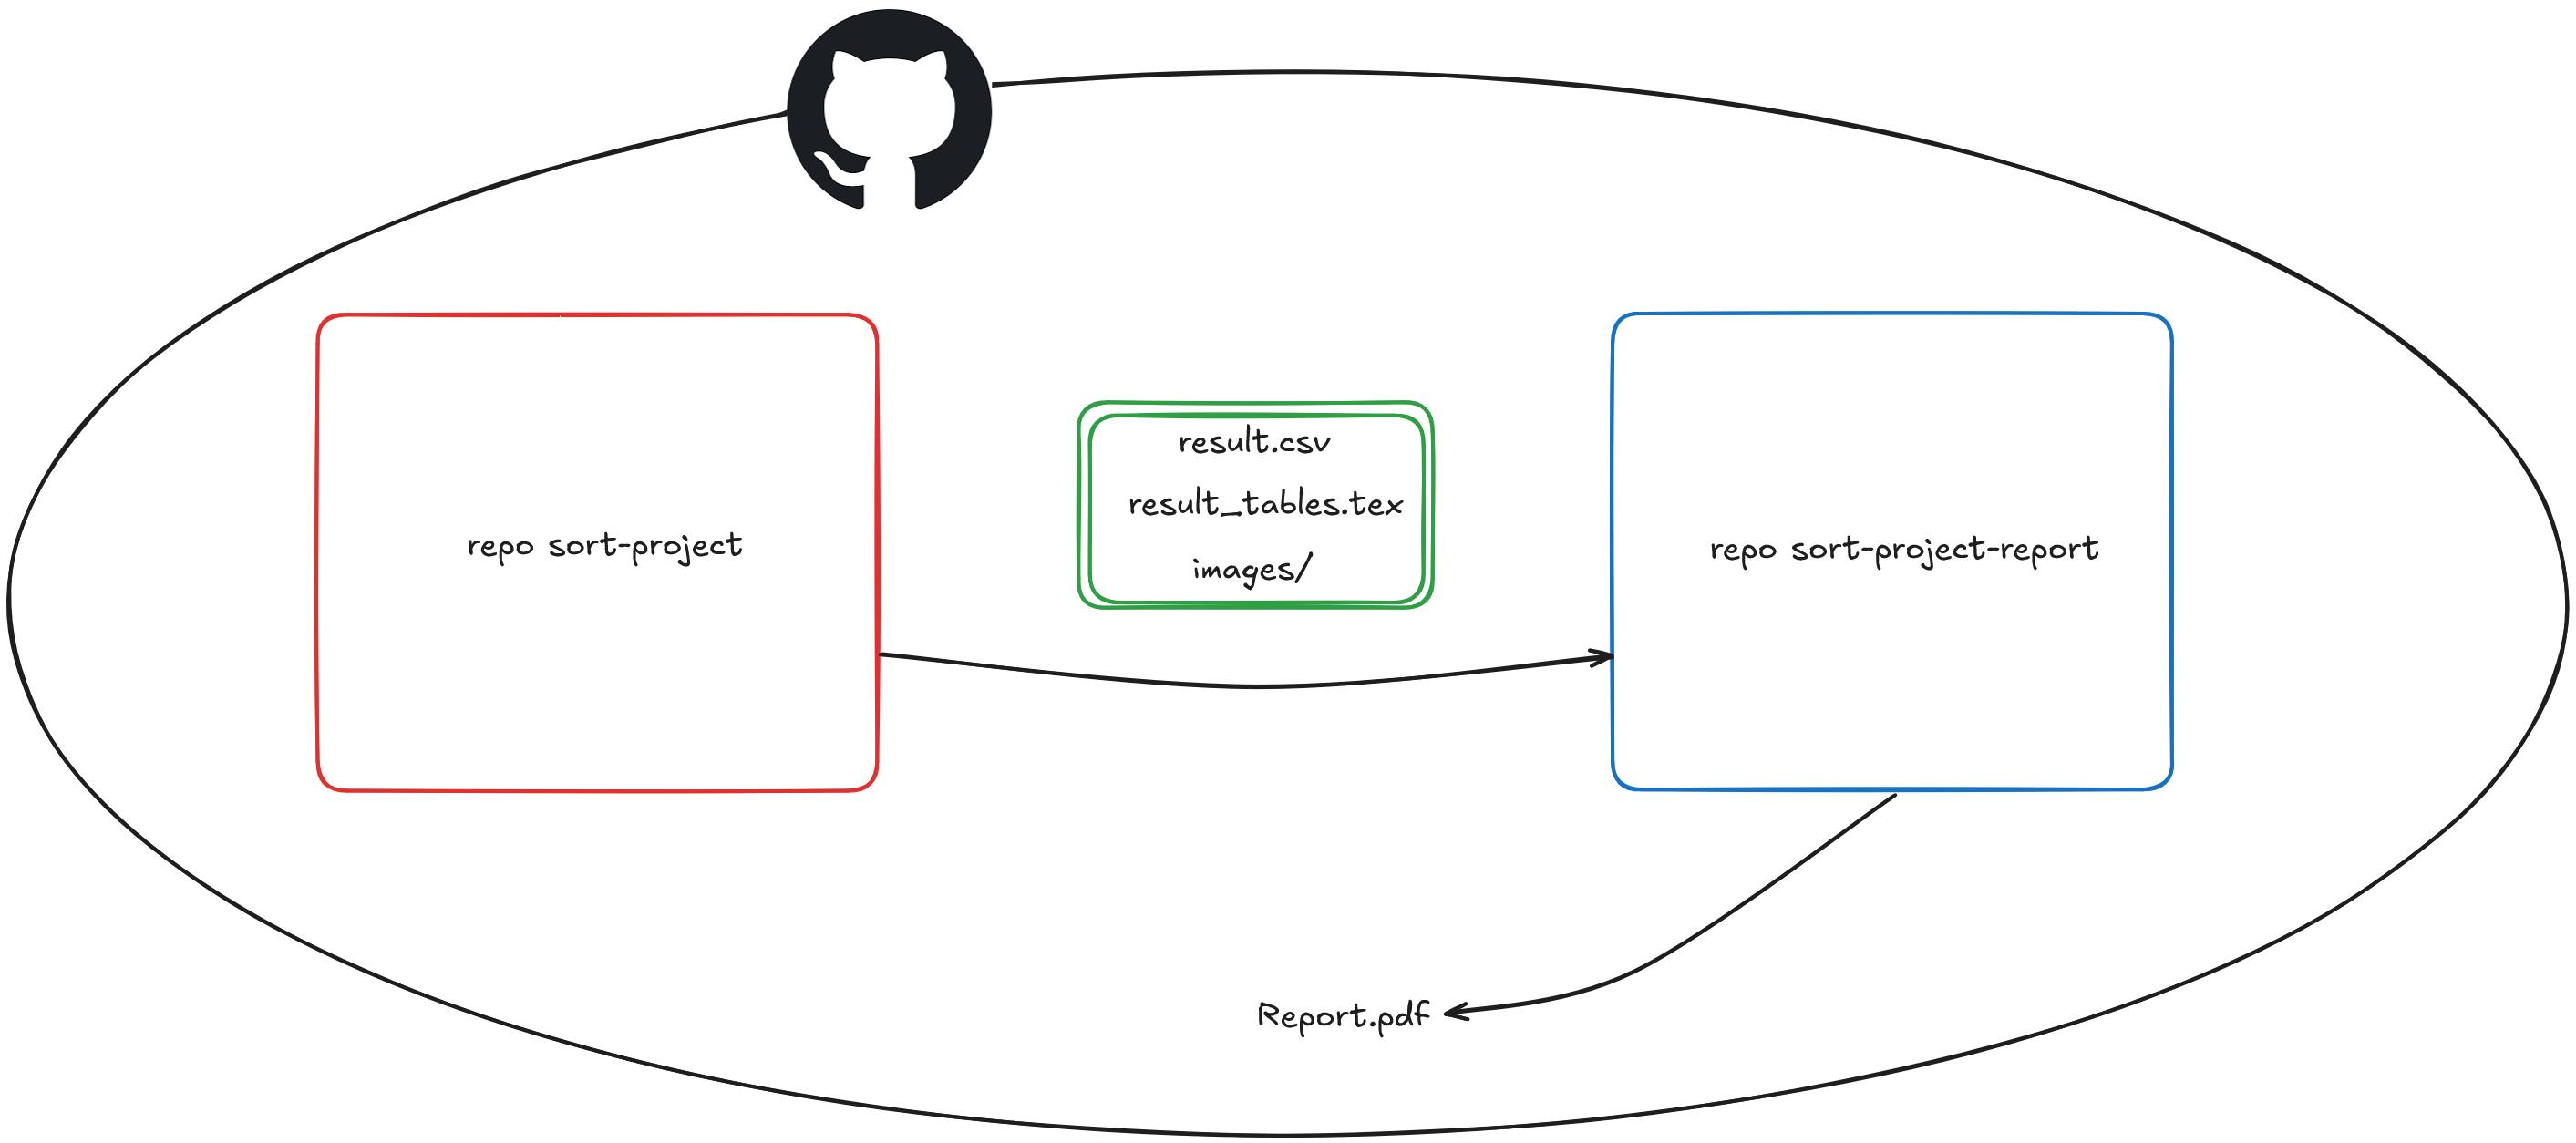
\includegraphics[width=\textwidth]{img/pipeline.png}
    \caption{Pipeline tạo ra số liệu cho thực nghiệm}
    \label{fig:pipeline}
\end{figure}

Pipeline này bao gồm hai file YAML chính:

\begin{itemize}
    \item \textbf{File YAML của repository sort-project}: File này được sử dụng để biên dịch, chạy và tạo release mới để chứa các file kết quả từ dự án C++ và Jupyter Notebook. Các bước chính bao gồm:
    \begin{itemize}
        \item Thiết lập môi trường MSVC và biên dịch file \texttt{run.cpp} thành \texttt{run.exe}.
        \item Chạy file \texttt{run.exe} để lấy được file \texttt{result.csv}.
        \item Thiết lập môi trường Python và cài đặt các thư viện cần thiết.
        \item Chạy Jupyter Notebook để chuyển file \texttt{result.csv} thành bảng latex và tạo ra các hình ảnh, biểu đồ cho báo cáo.
        \item Lưu trữ các file kết quả như \texttt{result.csv}, \texttt{result\_tables.tex} và thư mục \texttt{images}.
        \item Tạo một release mới trên GitHub và tải lên các file kết quả.
    \end{itemize}
    
    \item \textbf{File YAML của repository sort-project-report}: File này được sử dụng để biên dịch và tạo release mới để chứa file báo cáo. Các bước chính bao gồm:
    \begin{itemize}
        \item Tải các file \texttt{result.csv}, \texttt{result\_tables.tex} và thư mục \texttt{images} về từ release mới nhất của repository sort-project.
        \item Tải xuống và giải nén các file kết quả.
        \item Biên dịch tài liệu LaTeX thành file PDF.
        \item Đổi tên file PDF thành \texttt{Report.pdf}.
        \item Tạo một release mới trên GitHub và tải lên file \texttt{Report.pdf}.
    \end{itemize}
\end{itemize}

Với pipeline trên, việc thực hiện các thí nghiệm nhiều lần trở nên dễ dàng mà không lo ngại về việc quá tải máy tính, đồng thời cập nhật kết quả từ thí nghiệm vào báo cáo một cách nhanh chóng và tiết kiệm thời gian.
\end{document}